% =====================================================================
%  CeNTREX State Cleanup
%  Thesis-format summary of the design and optical-Bloch simulations of the two
%  rotational-state cleanup stages of CeNTREX: CU1 (X, J=1) and CU2 (X, J=2),
%  and of the first CU1 test on the SPB setup
%  Compile: latexmk -pdf main.tex   (or the LaTeX Workshop default recipe)
%  Figures: simulation figures in figures/ (made by scripts/), analysis figures of the
%  CU1 test in figures/experiment/; a framed placeholder names a figure still to be made.
% =====================================================================
\documentclass[11pt,a4paper,oneside]{report}

\usepackage[T1]{fontenc}
\usepackage{lmodern}
\usepackage[a4paper,left=30mm,right=25mm,top=28mm,bottom=28mm]{geometry}
\usepackage{setspace}
\onehalfspacing
\usepackage{amsmath,amssymb,bm}
\usepackage{graphicx}
\usepackage{booktabs,tabularx,multirow,array}
\newcolumntype{L}{>{\raggedright\arraybackslash}X}  % ragged-right X column
\usepackage[separate-uncertainty=true]{siunitx}
\DeclareSIUnit{\gauss}{G}
\usepackage{xcolor}
\usepackage[font=small,labelfont=bf]{caption}
\usepackage{subcaption}
\usepackage{float}
\usepackage{enumitem}
\setlist{itemsep=2pt,topsep=4pt}
\usepackage{fancyhdr}
\usepackage[nottoc]{tocbibind}
\usepackage[hidelinks]{hyperref}
\graphicspath{{figures/}}
\setlength{\emergencystretch}{3em}
% compact chapter headings (report default leaves ~170pt above the text)
\usepackage{titlesec}
\titleformat{\chapter}[display]{\normalfont\huge\bfseries\filright\hyphenpenalty=10000}{\chaptertitlename\ \thechapter}{10pt}{\Huge}
\titlespacing*{\chapter}{0pt}{0pt}{20pt}
% float placement: allow more floats per text page, fewer sparse float pages
\renewcommand{\topfraction}{0.9}
\renewcommand{\bottomfraction}{0.8}
\renewcommand{\textfraction}{0.07}
\renewcommand{\floatpagefraction}{0.85}
\setcounter{topnumber}{3}
\setcounter{bottomnumber}{2}
\setcounter{totalnumber}{5}
% float-only pages start at the top instead of being centred vertically
\makeatletter
\setlength{\@fptop}{0pt}
\setlength{\@fpsep}{14pt plus 4pt}
\setlength{\@fpbot}{0pt plus 1fil}
\makeatother

\pagestyle{fancy}
\fancyhf{}
\fancyhead[L]{\small\nouppercase{\leftmark}}
\fancyhead[R]{\small\thepage}
\renewcommand{\headrulewidth}{0.4pt}
\fancypagestyle{plain}{\fancyhf{}\fancyfoot[C]{\small\thepage}\renewcommand{\headrulewidth}{0pt}}

% ---- notation ---------------------------------------------------------
\newcommand{\code}[1]{\texttt{#1}}
\newcommand{\etac}{\eta_{\mathrm{c}}}
\newcommand{\Ngam}{N_{\gamma}}
\newcommand{\sigs}{\sigma_{s}}
\newcommand{\sigy}{\sigma_{y}}
\newcommand{\wmod}{\omega_{\mathrm{m}}}
\newcommand{\wpol}{\omega_{\mathrm{p}}}
\newcommand{\Dxb}{D_{XB}}
\newcommand{\fAOM}{f_{\mathrm{AOM}}}
\newcommand{\Dmain}{\Delta_{\mathrm{main}}}

% ---- figure placeholder -------------------------------------------------
% \figplaceholder[height]{expected file name}
% Replace by \includegraphics[width=\textwidth]{<file>} once the figure exists.
\newcommand{\figplaceholder}[2][0.30\textheight]{%
  \fbox{\begin{minipage}[c][#1][c]{0.95\textwidth}\centering
    {\color{gray}\Large Figure placeholder\par}\vspace{2mm}
    {\color{gray}\small\texttt{figures/\detokenize{#2}}\par}
  \end{minipage}}}

\begin{document}

% =====================================================================
\begin{titlepage}
\centering
\vspace*{25mm}
{\Huge\bfseries CeNTREX State Cleanup\par}
\vspace{10mm}
{\Large Design and optical-Bloch-equation simulations of the\\[2mm]
rotational-state cleanup stages CU1 ($J=1$) and CU2 ($J=2$),\\[2mm]
and a first test of CU1 on the SPB setup\par}
\vspace{30mm}
{\large Yuanhang Yang\par}
\vspace{4mm}
{\large CeNTREX Collaboration\par}
\vfill
{\large October 2026\par}
\vspace{10mm}
\end{titlepage}

% =====================================================================
\pagenumbering{roman}
\chapter*{Abstract}
\addcontentsline{toc}{chapter}{Abstract}

The CeNTREX experiment measures the Schiff moment of the $^{205}$Tl nucleus in a beam of
thallium fluoride. After the electrostatic lens the molecules are in $X(v{=}0)$, $J=2$, and
state preparation (SPB) transfers them to $J=1$, the level used in the interaction region.
Two state-cleanup stages bracket this transfer: CU1 removes the population of $J=1$ before
SPB, and CU2 removes the population left in $J=2$ after it. Both stages pump the molecules
through the $B\,{}^3\Pi_1$ state into other rotational levels, in the electric field that is
kept on to preserve the spin. In that field the Stark interaction spreads the excited-state
sublevels over tens of MHz, so that a single laser frequency leaves many ground-state
superpositions dark. This report documents how the two cleanup schemes were designed
around this problem, simulates both with Lindblad master equations using
\code{centrex-tlf} (0.2.5 and 0.3.0) and its native Rust solver, and compares the CU1 model with
a first test of CU1 on the SPB setup.

The model contains the complete field-dressed hyperfine structure of the addressed levels,
including both $\Lambda$-doublet components of $B$; decay into every rotational level of $X$
with branching ratios computed in the field; a 13-pass multipass beam with \SI{10}{\percent}
loss per pass; X/Z polarization switching at \SI{0.5}{MHz}; and phase modulation. A single
molecule at \SI{184}{m/s} is followed through \SI{5}{cm}. Its transverse velocity (with the
Doppler shift that alternates in sign from pass to pass) and transverse position are scanned
as well, and the results are averaged over the transverse distribution of a beam simulation
(lens at \SI{25}{kV}), counting only molecules inside the detection laser.

CU1 uses one laser on R(1) $F_1'=5/2$, $F'=2$ at \SI{150}{V/cm}, without phase modulation. On
the beam axis an \SI{80}{mW} beam removes \SI{99.96}{\percent} of the population at
$+\SI{20.2}{MHz}$ from the main resonance, but the optimum is only \SI{0.6}{MHz} wide at the
\SI{99.9}{\percent} level. Because the Doppler shift alternates in sign from pass to pass, CU1 is
therefore very sensitive to the transverse velocity (\SI{78}{\percent} at \SI{1}{m/s}), and
averaged over a transverse distribution the best detuning is $+\SI{19.0}{MHz}$, the set point.
There the laser is resonant with the eight SPB-related sublevels for molecules with
$|v_x|\approx\SI{0.5}{m/s}$, which are cleaned better than those at rest. With the lensed-beam
distribution assumed before the test ($\sigma_{v_x}=\SI{0.65}{m/s}$) the model predicts
\SI{98.7}{\percent} for an \SI{80}{mW}, \SI{3}{cm} beam and \SI{96.5}{\percent} for the
\SI{50}{mW}, \SI{2}{cm} beam of the test; a laser tilt must stay below about \SI{1}{mrad}.

In the test on the SPB setup (2026-10-16 to 10-21), with $J=1$ molecules prepared by AP1 and
detected on R(1) $F_1'=5/2$, $F'=3$, CU1 removed \SI{97.4(2)}{\percent} of the detected $F=2$
population at \SI{50}{mW}, measured with a shutter that blocks CU1 on alternate shots. The
improvement from \SI{90}{\percent} came from a realigned multipass with about 17 passes and from
the choice of the RC line. The remaining fraction grows only as $\exp(-kP^{0.45})$ with the power,
and a Doppler scan shows that the detected $J=1$ molecules have $\sigma_{v_x}=\SI{1.28}{m/s}$, twice
the assumed value: the lens hardly acts on them, and the wide test detection accepts
$|v_x|>\SI{1}{m/s}$. With this distribution the model with 17 passes and \SI{3.5}{\percent} loss per
pass reproduces the measured power dependence to within \SI{5}{\percent} at 30--\SI{50}{mW}. For the
acceptance of the final experiment ($|v_x|\leq\SI{0.22}{m/s}$) it predicts an efficiency above
\SI{99.9}{\percent}. With Q(1) $F_1'=1/2$, $F'=1$ detection, which couples all $J=1$ sublevels but
forms dark states during detection, the efficiency is \SI{95.1(4)}{\percent}.

CU2 drives R(2) $F_1'=7/2$, $F'=3$ (\SI{80}{mW}) and $F'=4$ (\SI{24}{mW}) with two beams
derived from one laser by an AOM ($200\pm\SI{15}{MHz}$), both phase-modulated at
\SI{17.5}{MHz} with $\beta=1.5$, in a \SI{2.4}{cm} high beam. The experiment now operates
CU2 at about \SI{200}{V/cm}. There the $F'=4$ main resonance lies \SI{211.83}{MHz} above the
$F'=3$ main resonance, compared with \SI{219.93}{MHz} at the original \SI{250}{V/cm}. The
detuning pair found at \SI{250}{V/cm} (\SI{99.99}{\percent} there) therefore gives only
\SI{92.9}{\percent} at \SI{200}{V/cm}. A two-dimensional optimisation of laser and AOM
frequency over the full AOM range finds \SI{99.85}{\percent} at $+\SI{11.5}{MHz}$ from the
$F'=3$ main resonance and $f_{\mathrm{AOM}}=\SI{191.0}{MHz}$, confirmed with tighter
tolerances. A nearly equivalent optimum, \SI{99.80}{\percent}, lies at
$f_{\mathrm{AOM}}=\SI{208.5}{MHz}$. Both are 2--\SI{3}{MHz} wide at the \SI{99}{\percent} level.
With the present \SI{3}{cm} beam and the transverse distribution within the detection
acceptance, the second optimum is the more robust one: at $f_{\mathrm{AOM}}=\SI{208.5}{MHz}$
CU2 removes \SI{96.7}{\percent} of a uniformly populated $J=2$ level and \SI{99.6}{\percent}
of the population left in the SPB source levels. For CU2 the transverse position matters more
than the transverse velocity.

\tableofcontents
\listoffigures
\listoftables

\cleardoublepage
\pagenumbering{arabic}

% =====================================================================
\chapter{Introduction}
\label{ch:intro}

\section{CeNTREX}

CeNTREX (Cold molecule Nuclear Time-Reversal EXperiment)~\cite{Grasdijk2021} searches for
the Schiff moment of the $^{205}$Tl nucleus, a CP-violating nuclear moment, by measuring a
CP-odd frequency shift in thallium fluoride (TlF). It uses a cryogenic buffer-gas beam of
TlF, rotational cooling, an electrostatic lens, state preparation, a Ramsey measurement in a
strong electric field and laser-induced-fluorescence detection. Every step relies on the
molecules being in well-defined rotational and hyperfine levels of the ground electronic
state.

\section{State cleanup in the CeNTREX beamline}
\label{sec:beamline}

The molecules leave the electrostatic lens in $X(v{=}0)$, $J=2$. The state-preparation stage
SPB then transfers them from $J=2$ to $J=1$, the rotational level used in the interaction
region. Two cleanup stages bracket this transfer (Fig.~\ref{fig:beamline}):
\begin{itemize}
  \item \textbf{CU1}, before SPB, pumps off the population of $J=1$. Molecules already in
        $J=1$ would otherwise reach the interaction region together with the transferred ones.
  \item \textbf{CU2}, after SPB, pumps off the population that remains in $J=2$.
\end{itemize}
Ideally the cleanup would also remove the other sublevels of $J=2$ before SPB and of $J=1$
after it, except the target state. That would require a broadband UV EOM and is not
pursued.

A cleanup stage removes the population of a rotational level by optical pumping. The
molecules cross a laser resonant with a transition from that level to $B\,{}^3\Pi_1$. Each
excitation is followed by spontaneous decay, and because $B$ decays to several rotational
levels of $X$, most decays end in a level that the light does not address. The remaining
decays return the molecule to the addressed level, where it can be excited again. A few
photons per molecule therefore suffice, provided that every sublevel of the addressed level
is excited and none is left in a dark superposition.

To preserve the spin, the electric field is kept non-zero until the end of the beamline, so
both stages pump in an electric field: about \SI{150}{V/cm} for CU1 and, in the present
configuration, about \SI{200}{V/cm} for CU2 (\SI{250}{V/cm} in the original design). In the
field the Stark interaction moves the hyperfine sublevels of the excited state apart by tens
of MHz, many natural linewidths. A single laser frequency then reaches only a few of them,
and more ground-state superpositions are dark. The design of both schemes
(Chapter~\ref{ch:design}) is mainly a response to this problem.

\begin{figure}[htbp]
  \centering
  \figplaceholder[0.16\textheight]{beamline_cleanup_stages.pdf}
  \caption[Cleanup stages in the CeNTREX beamline]{Cleanup stages in the CeNTREX beamline:
  lens ($J=2$) $\to$ CU1 (removes $J=1$) $\to$ SPB ($J=2\to J=1$) $\to$ CU2 (removes $J=2$)
  $\to$ interaction region ($J=1$). Design-study slide~2~\cite{CleanupTheory2024}.}
  \label{fig:beamline}
\end{figure}

\section{Scope of this work}

The aims are
\begin{enumerate}
  \item to document the design of the two cleanup schemes;
  \item to set up a complete optical-Bloch model of each stage, with the field-dressed level
        structure, the multipass beam geometry, polarization switching, phase modulation and,
        for CU2, the AOM coupling of the two beams;
  \item to find the laser frequencies that maximise the cleanup efficiency within the
        hardware limits, and the width of the optimum;
  \item to establish which approximations the results depend on, and to check the numerics;
  \item to test CU1 on the SPB setup and compare the measurement with the model.
\end{enumerate}

All simulations use the baseline parameters of Table~\ref{tab:baseline}. The model is a
single-trajectory model: one molecule at the mean forward velocity. The transverse velocity,
with its Doppler shift, and the transverse position are scanned, and the results are averaged
over the transverse distribution of a beam simulation within the detection acceptance
(CU1: Secs.~\ref{sec:j1_avg}--\ref{sec:j1_present}; CU2: Sec.~\ref{sec:j2_doppler}).
\textbf{Three sets of beam parameters appear in this report.} The design-level results (detuning,
power and the two-dimensional CU2 optimisation) use \SI{4.8}{cm} for CU1 and \SI{2.4}{cm} for CU2.
In the experiment both beams were then about \SI{3}{cm} high (Secs.~\ref{sec:j1_present}
and~\ref{sec:j2_doppler}), and CU1 was tested with \SI{50}{mW} in a \SI{2}{cm} beam
(Sec.~\ref{sec:j1_present} and Chapter~\ref{ch:j1_exp}). The test also measured three inputs that
the simulations had assumed: the transverse velocity spread of the detected $J=1$ molecules, the
forward velocity and the number of passes (Sec.~\ref{sec:exp_model}).

\begin{table}[htbp]
  \centering
  \caption[Baseline parameters]{Baseline parameters of this report. Beam heights are full
  $4\sigma$ widths.}
  \label{tab:baseline}
  \small
  \begin{tabularx}{\textwidth}{lLL}
    \toprule
    & CU1 ($J=1$) & CU2 ($J=2$) \\
    \midrule
    electric field & \SI{150}{V/cm} & \SI{200}{V/cm} \\
    transition(s) & R(1) $F_1'=5/2$, $F'=2$ & R(2) $F_1'=7/2$, $F'=3$ and $F'=4$ \\
    laser power & \SI{80}{mW}; test: \SI{50}{mW} & \SI{80}{mW} ($F'=3$) + \SI{24}{mW} ($F'=4$) \\
    beam height & \SI{4.8}{cm}; present: \SI{3}{cm}; test: \SI{2}{cm} (Sec.~\ref{sec:j1_present}) & \SI{2.4}{cm}; present: \SI{3}{cm} (Sec.~\ref{sec:j2_doppler}) \\
    detuning & $+\SI{20.2}{MHz}$ on axis; set point $+\SI{19.0}{MHz}$ & optima R1 and R2 (Sec.~\ref{sec:j2_2d}) \\
    phase modulation & none & \SI{17.5}{MHz}, $\beta=1.5$, common to both beams \\
    AOM & -- & $\fAOM=200\pm\SI{15}{MHz}$ \\
    \midrule
    multipass & \multicolumn{2}{l}{13 passes, \SI{10}{\percent} loss per pass, \SI{3}{mm} wide along the molecular beam} \\
    & \multicolumn{2}{l}{(CU1 test: about 17 passes, 3.5--\SI{4.5}{\percent} loss per pass fitted; Sec.~\ref{sec:exp_model})} \\
    polarization & \multicolumn{2}{l}{X/Z switching at \SI{0.5}{MHz}} \\
    molecule & \multicolumn{2}{l}{\SI{184}{m/s} on the beam axis, \SI{5}{cm} interaction length (CU1 test: \SI{145}{m/s})} \\
    transverse motion & $v_x$ and $y_0$ scanned (Secs.~\ref{sec:j1_doppler}, \ref{sec:j1_present}) & $v_x$ and $y_0$ scanned at the optima (Sec.~\ref{sec:j2_doppler}) \\
    transverse distribution & beam sim.\ (\SI{25}{kV}): $\sigma_{v_x}=\SI{0.65}{m/s}$, $\sigma_y=\SI{10.95}{mm}$; measured for $J=1$ in the test: $\sigma_{v_x}=\SI{1.28}{m/s}$ & beam sim.\ (\SI{25}{kV}): $\sigma_{v_x}=\SI{0.65}{m/s}$, $\sigma_y=\SI{10.35}{mm}$ \\
    detection acceptance & \multicolumn{2}{l}{$|v_x|\leq\SI{1}{m/s}$, $|y_0|\leq\SI{8.5}{mm}$ (detection laser \SI{1.7}{cm} high)} \\
    & \multicolumn{2}{l}{(CU1 test: $|v_x|$ up to 1.2--\SI{1.7}{m/s}; final experiment: $|v_x|\leq\SI{0.22}{m/s}$)} \\
    \bottomrule
  \end{tabularx}
\end{table}

\section{Outline}

\begin{itemize}[itemsep=1pt]
  \item Chapter~\ref{ch:system} introduces the TlF levels, the cleanup transitions and their
        structure in the applied field.
  \item Chapter~\ref{ch:design} describes how the two schemes were designed, and the
        operating constraints, in particular the AOM coupling of the CU2 beams.
  \item Chapter~\ref{ch:sim} describes the simulation in detail and summarises every
        assumption.
  \item Chapter~\ref{ch:j1} presents the CU1 simulation, Chapter~\ref{ch:j1_exp} the test of CU1
        on the SPB setup and its comparison with the model, and Chapter~\ref{ch:j2} the CU2 results
        at \SI{200}{V/cm}.
  \item Chapter~\ref{ch:checks} collects the numerical checks, and
        Chapter~\ref{ch:conclusion} concludes. The appendices give the full parameter list,
        the line positions of the CU1 test, the \SI{250}{V/cm} reference results and the code and
        data structure.
\end{itemize}

% =====================================================================
\chapter{Physical system}
\label{ch:system}

\section{The TlF states}

The ground electronic state $X\,{}^1\Sigma^+$ ($\Omega=0$) and the excited state
$B\,{}^3\Pi_1$ ($\Omega=\pm1$) both carry hyperfine structure from the two nuclear spins,
$I_{\mathrm{Tl}}=I_{\mathrm F}=1/2$. Following the \code{centrex-tlf}
conventions~\cite{centrextlf}, the spins couple to the rotation in two steps,
$\mathbf J+\mathbf I_1=\mathbf F_1$ and $\mathbf F_1+\mathbf I_2=\mathbf F$, and states are
labelled $|J,F_1,F,m_F,P\rangle$. Each rotational level of $X$ has a single parity
$P=(-1)^J$. Each rotational level $J'$ of $B$ is a $\Lambda$-doublet with one component of
each parity. The $\Lambda$-doubling is small, so the two components are strongly mixed by
electric fields of a few hundred V/cm. Primed quantum numbers refer to $B$. A transition is
named by its branch and the ground-state $J$: R($J$) is $J\to J'=J+1$.

At zero field the $J=1$ level has 12 sublevels ($F_1=1/2$: $F=0,1$; $F_1=3/2$: $F=1,2$), and
$J=2$ has 20 ($F_1=3/2$: $F=1,2$; $F_1=5/2$: $F=2,3$).

\section{The cleanup transitions}

Table~\ref{tab:transitions} lists the transitions and the \emph{main} state pairs. The main
pair of a laser fixes the zero of its detuning axis and normalises its Rabi rate
(Sec.~\ref{sec:couplings}). Its matrix element $m$, in units of the reduced $X$--$B$
transition dipole moment, is evaluated between the field-dressed states for X polarization.

\begin{table}[htbp]
  \centering
  \caption[Cleanup transitions and main state pairs]{Cleanup transitions, main state pairs
  and main-pair matrix elements $m$ (X polarization, field-dressed states).}
  \label{tab:transitions}
  \small
  \begin{tabularx}{\textwidth}{llLc}
    \toprule
    stage & transition & main pair $|J,F_1,F,m_F\rangle\to|J',F_1',F',m_F',P'\rangle$ & $|m|$ \\
    \midrule
    CU1, \SI{150}{V/cm} & R(1) $F_1'=5/2$, $F'=2$ &
      $|1,\tfrac32,2,1\rangle\to|2,\tfrac52,2,2,+\rangle$ & 0.1004 \\
    CU2, \SI{200}{V/cm}, beam 0 & R(2) $F_1'=7/2$, $F'=3$ &
      $|2,\tfrac52,3,2\rangle\to|3,\tfrac72,3,3,-\rangle$ & 0.0948 \\
    CU2, \SI{200}{V/cm}, beam 1 & R(2) $F_1'=7/2$, $F'=4$ &
      $|2,\tfrac52,3,0\rangle\to|3,\tfrac72,4,1,-\rangle$ & 0.2286 \\
    \bottomrule
  \end{tabularx}
\end{table}

\section{Structure in the applied field}
\label{sec:dressed}

The cleanup takes place in a static electric field $\mathbf E=E\hat{\mathbf z}$, which defines
the quantisation axis. With $\mathbf E$ and the small magnetic field both along $z$, $m_F$
remains a good quantum number. $J$, $F_1$, $F$ and, in $B$, the parity are mixed. In the
ground state the hyperfine structure of each rotational level spans only a few MHz
(\SI{2.4}{MHz} for $J=1$ at \SI{150}{V/cm}, \SI{1.4}{MHz} for $J=2$ at \SI{250}{V/cm}). In
the excited state the $|m_F'|$ sublevels of one hyperfine level are split by the Stark
interaction by about \num{10}--\SI{25}{MHz} each (Chapter~\ref{ch:design}), much more than the
natural linewidth $\Gamma/2\pi=\SI{1.61}{MHz}$.

Table~\ref{tab:spread} gives the positions of all transition components with a
non-negligible matrix element, measured from the main resonance of the beam that drives them.
These positions set the optimum detunings and are the reason for phase modulation in CU2.

\begin{table}[htbp]
  \centering
  \caption[Spread of the transition components in the applied field]{Spread of the
  transition components (pairs with $|M_{eg}|^2>10^{-4}\max|M_{eg}|^2$, X and Z polarization
  combined) relative to the main resonance of the beam that drives them, and their mean
  weighted by $|M_{eg}|^2$. Computed from the rotating-frame Hamiltonian of the OBE system.}
  \label{tab:spread}
  \small
  \begin{tabular}{lcccc}
    \toprule
    system & pairs & lowest & highest & weighted mean \\
    \midrule
    CU1, \SI{150}{V/cm}, addressed parity only & 32 & \SI{0.0}{MHz} & \SI{34.2}{MHz} & \SI{19.5}{MHz} \\
    CU1, \SI{150}{V/cm}, both parities & 62 & \SI{0.0}{MHz} & \SI{79.9}{MHz} & \SI{33.3}{MHz} \\
    CU2, \SI{200}{V/cm}, beam 0 ($F'=3$) & 106 & \SI{0.0}{MHz} & \SI{86.9}{MHz} & \SI{40.7}{MHz} \\
    CU2, \SI{200}{V/cm}, beam 1 ($F'=4$) & 106 & $-\SI{31.4}{MHz}$ & \SI{55.5}{MHz} & \SI{8.9}{MHz} \\
    \bottomrule
  \end{tabular}
\end{table}

For CU2 the two beams address different excited hyperfine levels. Their main resonances are
separated by
\begin{equation}
  \Dmain(E)=\frac{\bigl(E_{e_0}-E_{g_0}\bigr)_1-\bigl(E_{e_0}-E_{g_0}\bigr)_0}{2\pi}
  =\begin{cases}\SI{211.83}{MHz}, & E=\SI{200}{V/cm},\\ \SI{219.93}{MHz}, & E=\SI{250}{V/cm},\end{cases}
  \label{eq:dmain}
\end{equation}
with the $F'=4$ resonance above the $F'=3$ one. The physical frequency difference of the two
beams is therefore
\begin{equation}
  \frac{\omega_1-\omega_0}{2\pi}=\Dmain(E)+\frac{\delta_1-\delta_0}{2\pi},
  \label{eq:laser_separation}
\end{equation}
with $\delta_k$ the detuning of beam $k$ from its own main resonance. In the experiment this
difference is the AOM frequency (Sec.~\ref{sec:aom}).

\begin{figure}[htbp]
  \centering
  \figplaceholder{level_diagram_CU1_R1_F2_150Vcm.pdf}
  \caption[Field-dressed level diagram, CU1]{Field-dressed $X\to B$ level diagram for R(1)
  $F_1'=5/2$, $F'=2$ at \SI{150}{V/cm}, with each level segmented by its zero-field parent
  character (to be generated with \code{utils.plotting.plot\_transition\_level\_diagram}).}
  \label{fig:levels_j1}
\end{figure}

\begin{figure}[htbp]
  \centering
  \figplaceholder{level_diagram_CU2_R2_F3F4_200Vcm.pdf}
  \caption[Field-dressed level diagram, CU2]{As Fig.~\ref{fig:levels_j1} for R(2)
  $F_1'=7/2$, $F'=3$ and $F'=4$ at \SI{200}{V/cm}.}
  \label{fig:levels_j2}
\end{figure}

\begin{figure}[htbp]
  \centering
  \figplaceholder{stick_spectra_CU1_CU2.pdf}
  \caption[Transition components versus detuning]{Stick spectra of the transition
  components of Table~\ref{tab:spread}: position on each beam's detuning axis and
  $|M_{eg}|^2$ relative to the main pair. (a) CU1 at \SI{150}{V/cm}. (b) CU2 at
  \SI{200}{V/cm}, beams 0 and 1, with the carriers and their phase-modulation sidebands.}
  \label{fig:sticks}
\end{figure}

\section{Field mixing of the ground-state hyperfine levels}
\label{sec:gmixing}

The field also mixes the ground-state hyperfine levels, which matters for the cleanup because
it opens transitions that are forbidden at zero field. The clearest case is
$|J=1,F_1=\tfrac12,F=0,m_F=0\rangle$. At zero field it cannot be excited to $F'=2$
($\Delta F=2$). In the field it acquires an admixture of $|J=1,F_1=\tfrac32,F=2,m_F=0\rangle$
(Table~\ref{tab:f0mix}), which at \SI{150}{V/cm} carries \SI{29}{\percent} of the
probability, and this admixture is what CU1 pumps. The same mechanism lets CU2 pump the $F=1$
sublevels of $J=2$ to $F'=3$, through their admixture of $F=3$ (Sec.~\ref{sec:design_cu2}).

\begin{table}[htbp]
  \centering
  \caption[Field mixing of the $J=1$, $F=0$ ground state]{Composition of the field-dressed
  state $|J=1,F_1=\tfrac12,F=0,m_F=0\rangle$ (amplitudes) versus electric field
  (design study~\cite{CleanupTheory2024}, slide~9).}
  \label{tab:f0mix}
  \small
  \begin{tabular}{lcc}
    \toprule
    $E$ & $|F_1=\tfrac12,F=0,m_F=0\rangle$ & $|F_1=\tfrac32,F=2,m_F=0\rangle$ \\
    \midrule
    \SI{0}{V/cm} & 1.00 & -- \\
    \SI{20}{V/cm} & 1.00 & 0.08 \\
    \SI{40}{V/cm} & 0.97 & 0.26 \\
    \SI{150}{V/cm} & 0.84 & 0.54 \\
    \bottomrule
  \end{tabular}
\end{table}

\section{Branching ratios}

Table~\ref{tab:br} gives the decay branching ratios of the addressed excited levels into the
rotational levels of $X$, computed between the field-dressed states. They show why a few
photons suffice: from $F'=2$ of $B$, $J'=2$ only \SI{37}{\percent} of the decays return to
$J=1$, and from $F'=3$ or $F'=4$ of $J'=3$ only \SI{27}{\percent} return to $J=2$. The
field-dressed $B$ levels contain a large opposite-parity admixture. Even when only the
addressed parity is kept as a dynamical level (CU1 row), \SI{28}{\percent} of the decays go
to $J=2$, which is parity-forbidden at zero field.

\begin{table}[htbp]
  \centering
  \caption[Branching ratios]{Branching ratios of the addressed $B$ levels into the
  rotational levels of $X(v{=}0)$ in the applied field. For the CU2 levels both
  $\Lambda$-doublet components are retained and the ratios are summed over all excited
  sublevels of the level and normalised.}
  \label{tab:br}
  \small
  \begin{tabular}{lcccccc}
    \toprule
    excited level & $J=0$ & $J=1$ & $J=2$ & $J=3$ & $J=4$ & $J=5$ \\
    \midrule
    $J'=2$, $F'=2$, $P'=+$ (\SI{150}{V/cm}) & 0.00005 & \textbf{0.371} & 0.280 & 0.334 & 0.016 & -- \\
    $J'=3$, $F'=3$ (\SI{200}{V/cm}) & -- & 0.00002 & \textbf{0.265} & 0.484 & 0.235 & 0.016 \\
    $J'=3$, $F'=4$ (\SI{200}{V/cm}) & -- & 0.00001 & \textbf{0.265} & 0.484 & 0.235 & 0.016 \\
    \bottomrule
  \end{tabular}
\end{table}

% =====================================================================
\chapter{Design of the cleanup schemes}
\label{ch:design}

The two schemes were designed in an earlier study~\cite{CleanupTheory2024}. That study used
the previous, Julia-based version of the OBE code and treated CU2 at the original field of
\SI{250}{V/cm}. Some of its assumptions differ from the present baseline: other laser powers
and beam heights, and \SI{5}{\percent} loss per pass in its final comparison. Its numbers are
quoted in this chapter because they explain the choices. The results for the present baseline
are in Chapters~\ref{ch:j1} and~\ref{ch:j2}.

\section{Dark states and how to avoid them}
\label{sec:darkstates}

For a fixed laser polarization and frequency, $N_g$ ground sublevels coupled to $N_e$ excited
sublevels leave at least $N_g-N_e$ ground-state superpositions that do not couple to the light.
Molecules in them are never pumped. In the field, $N_e$ counts only the excited sublevels
that lie within reach of the laser spectrum, because the Stark splitting moves the others tens
of MHz away. Three tools reduce the problem, and both schemes use all of them:
\begin{enumerate}
  \item \textbf{reach enough excited sublevels}, with the carrier placed between them, with
        phase-modulation sidebands, or with a second beam on a second excited hyperfine level;
  \item \textbf{switch the polarization} between X and Z at \SI{500}{kHz}, so that a
        superposition dark for one polarization is bright for the other;
  \item \textbf{use field mixing}, which makes zero-field-forbidden transitions driveable
        (Sec.~\ref{sec:gmixing}).
\end{enumerate}

\section{CU1: one laser without phase modulation}
\label{sec:design_cu1}

At \SI{150}{V/cm} the five sublevels of $B$, $J'=2$, $F_1'=5/2$, $F'=2$, $P'=+$ form three
groups: $m_F'=0$ highest, $|m_F'|=1$ \SI{17.4}{MHz} below it and $|m_F'|=2$ a further
\SI{24.4}{MHz} below. The 12 sublevels of $J=1$ span \SI{2.4}{MHz} (Fig.~\ref{fig:cu1_scheme}).

\paragraph{Starting idea.} One laser with a resonant EOM whose two first-order sidebands reach
the $m_F'=0$ and $|m_F'|=2$ sublevels: $\Delta_{\mathrm{EOM}}=(17.4+24.4)/2=\SI{20.9}{MHz}$,
with the carrier \SI{3.5}{MHz} below the $|m_F'|=1$ pair.

\paragraph{Result.} Scans of laser detuning against EOM frequency at 10, 35, 60, 85 and
\SI{110}{mW} (Fig.~\ref{fig:cu1_eomscan}) put the minimum of the remaining population at
\emph{zero} modulation frequency for every power, at a detuning of about $+\SI{20}{MHz}$.
A single unmodulated frequency near the $|m_F'|=1$ pair is enough; the outer sublevels need
not be addressed directly. The $F=0$ sublevel, which cannot reach $F'=2$ at zero field, is
pumped through its field-induced $F=2$ admixture (Table~\ref{tab:f0mix}). All 12 sublevels
are emptied within the first $\sim\SI{2}{cm}$ of the interaction region.

\paragraph{Beam height.} At \SI{80}{mW} with a \SI{3}{mm}\,$\times$\,\SI{2.4}{cm} beam the
cleanup is complete for $|y_0|\lesssim\SI{0.6}{cm}$, but the remaining population rises to
about 0.12 at $|y_0|=\SI{1.2}{cm}$. With a \SI{4.8}{cm} beam it is 0.005 on axis and 0.028 at
$|y_0|=\SI{1.2}{cm}$. CU1 uses the \SI{4.8}{cm} beam.

\paragraph{Opposite parity.} With the $\Lambda$-doublet partner included, the detuning scan
shows a second group of peaks, from the opposite-parity component, between $+50$ and
$+\SI{80}{MHz}$; the optimum at $+\SI{20}{MHz}$ is unchanged (Chapter~\ref{ch:j1}).

\paragraph{Setup.} Frequency-doubled laser $\to$ polarization EOM (\SI{500}{kHz}) $\to$
multipass (Fig.~\ref{fig:setups}a).

\begin{figure}[htbp]
  \centering
  \figplaceholder{design_CU1_scheme.pdf}
  \caption[CU1 design: level scheme]{CU1 design. (a) Levels of $X$, $J=1$ and of $B$,
  $J'=2$, $F_1'=5/2$, $F'=2$ at \SI{150}{V/cm}. (b) Simplified scheme: five excited
  sublevels split by 17.4 and \SI{24.4}{MHz}, 12 ground sublevels within \SI{2.4}{MHz}, and the
  initial EOM idea. Design-study slides~3--5~\cite{CleanupTheory2024}.}
  \label{fig:cu1_scheme}
\end{figure}

\begin{figure}[htbp]
  \centering
  \figplaceholder{design_CU1_EOM_scan.pdf}
  \caption[CU1 design: detuning versus EOM frequency]{CU1 design: remaining $J=1$
  population versus laser detuning and EOM frequency at 10, 35, 60, 85 and \SI{110}{mW}. The
  minimum lies at zero modulation and about $+\SI{20}{MHz}$ at every power. Design-study
  slides~6 and~8~\cite{CleanupTheory2024}.}
  \label{fig:cu1_eomscan}
\end{figure}

\section{CU2: from one laser to two hyperfine levels}
\label{sec:design_cu2}

At \SI{250}{V/cm} the sublevels of $B$, $J'=3$, $F_1'=7/2$, $F'=3$, $P'=-$ are split by about
\SI{18}{MHz} per step in $|m_F'|$, and the 20 sublevels of $J=2$ span \SI{1.4}{MHz}. The scheme
was developed in the steps of Table~\ref{tab:cu2_design}.

\begin{enumerate}
  \item \textbf{One laser on $F'=3$ with a resonant EOM.} The best point (EOM
        $\approx\SI{17}{MHz}$, $\beta\approx1.4$--1.6, detuning $\approx\SI{18.5}{MHz}$, \SI{100}{mW})
        cleans only about \SI{98}{\percent}. The bottleneck is
        $|J=2,F_1=\tfrac32,F=1,m_F=0\rangle$, which keeps about a fifth of its population. An
        $F=1$ sublevel reaches $F'=3$ only through its admixture of $F=3$, and $m_F=0$ reaches
        only $m_F'=\pm1$, through the EOM sidebands.
  \item \textbf{A weak second tone on $F'=3$, $m_F'=0$, made with an AOM.} With
        \SI{10}{mW} and Z polarization it helps only at a single, narrow detuning, where the
        remaining population falls from \SI{1.35}{\percent} to \SI{0.76}{\percent}. Three ground
        sublevels couple to a single excited sublevel and quickly form a dark state, and with a
        fixed Z polarization the polarization switching is not used.
  \item \textbf{Second beam on $F'=4$ instead.} The $F'=4$ level lies about \SI{200}{MHz}
        above $F'=3$. With \SI{70}{mW} on $F'=3$ and \SI{10}{mW} on $F'=4$, the scan of the
        second beam shows dips at the $F'=4$ $m_F'$ components (spaced by 11 and \SI{15}{MHz}
        near the top of the manifold), with \SI{0.6}{\percent} remaining at the best one, and
        the $m_F=0$ bottleneck is removed with the same total power. The cost is a UV AOM at about \SI{200}{MHz} with some tuning range.
  \item \textbf{Phase-modulate the second beam as well.} A second EOM on the $F'=4$ beam
        ($\approx\SI{11.5}{MHz}$, $\beta=2$) raises the cleanup above \SI{99.9}{\percent}
        (70 + \SI{10}{mW}). It stays above \SI{99}{\percent} at 50 + \SI{7}{mW} and reaches
        \SI{99.95}{\percent} at 60 + \SI{18}{mW}: the scheme works better with more power in
        the second beam.
  \item \textbf{One EOM for both beams.} With \SI{17.5}{MHz}, $\beta=1.5$ on both beams
        (60 + \SI{18}{mW}) the cleanup is still about \SI{99.6}{\percent}. A single EOM placed
        before the AOM is much simpler and was adopted.
  \item \textbf{Final comparison} (single EOM, \SI{5}{\percent} loss per pass, 50 +
        \SI{20}{mW}): \SI{99.8}{\percent} with a \SI{4}{cm} high beam, \SI{99.95}{\percent}
        with \SI{3}{cm}.
  \item \textbf{Present code with the $\Lambda$-doublet partners}, 80 + \SI{24}{mW},
        \SI{2.4}{cm}, \SI{10}{\percent} loss: \SI{99.99}{\percent} at the chosen point
        $(\delta_0,\delta_1)/2\pi=(+18.5,-\SI{6.5}{MHz})$ (Appendix~\ref{app:legacy}). A
        two-dimensional detuning map at this setting shows a lattice of optima, with the
        \SI{17.5}{MHz} EOM period along the $F'=3$ axis.
\end{enumerate}

\begin{table}[htbp]
  \centering
  \caption[CU2 design steps]{CU2 design steps at \SI{250}{V/cm} (design
  study~\cite{CleanupTheory2024}, except the last row). Powers are $F'=3$ + second beam.}
  \label{tab:cu2_design}
  \small
  \begin{tabularx}{\textwidth}{c>{\raggedright\arraybackslash}p{0.27\textwidth}L>{\raggedright\arraybackslash}p{0.21\textwidth}}
    \toprule
    step & beams & phase modulation & cleanup \\
    \midrule
    1 & $F'=3$, \SI{100}{mW} & one EOM, $\approx\SI{17}{MHz}$, $\beta\approx1.5$ & $\approx\SI{98}{\percent}$ \\
    2 & + $F'=3$, $m_F'=0$ tone, \SI{10}{mW}, Z & second tone unmodulated & \SI{99.24}{\percent} at one narrow detuning \\
    3 & $F'=3$ + $F'=4$, 70 + \SI{10}{mW} & EOM on $F'=3$ only & $\approx\SI{99.4}{\percent}$; $m_F=0$ bottleneck removed \\
    4 & 70 + \SI{10}{mW} / 50 + \SI{7}{mW} / 60 + \SI{18}{mW} & + EOM2 $\approx\SI{11.5}{MHz}$, $\beta=2$ on $F'=4$ & $>\SI{99.9}{\percent}$ / $>\SI{99}{\percent}$ / \SI{99.95}{\percent} \\
    5 & 60 + \SI{18}{mW} & one EOM, \SI{17.5}{MHz}, $\beta=1.5$, both beams & $\approx\SI{99.6}{\percent}$ \\
    6 & 50 + \SI{20}{mW}, 4\,/\,\SI{3}{cm}, \SI{5}{\percent} loss & as 5 & \SI{99.8}{\percent} / \SI{99.95}{\percent} \\
    7 & 80 + \SI{24}{mW}, \SI{2.4}{cm}, \SI{10}{\percent} loss & as 5; present code, both parities & \SI{99.99}{\percent} \\
    \bottomrule
  \end{tabularx}
\end{table}

\begin{figure}[htbp]
  \centering
  \figplaceholder{design_CU2_single_laser.pdf}
  \caption[CU2 design: one laser with an EOM]{CU2 design, step 1 (\SI{250}{V/cm},
  \SI{100}{mW}). (a) Remaining $J=2$ population versus detuning and EOM frequency. (b)
  Sublevel populations along the interaction region: $|F_1=\tfrac32,F=1,m_F=0\rangle$ is not
  cleaned. Design-study slides~17 and~19~\cite{CleanupTheory2024}.}
  \label{fig:cu2_step1}
\end{figure}

\begin{figure}[htbp]
  \centering
  \figplaceholder{design_CU2_second_beam.pdf}
  \caption[CU2 design: second beam on $F'=4$ and second EOM]{CU2 design, steps 3--5. (a)
  Remaining $J=2$ population versus the detuning of the $F'=4$ beam (70 + \SI{10}{mW}), with
  the dips assigned to $F'=4$ sublevels. (b) Detuning of the $F'=4$ beam versus frequency of
  its EOM. Design-study slides~23--27 and~31~\cite{CleanupTheory2024}.}
  \label{fig:cu2_step3}
\end{figure}

\section{Optical layouts}
\label{sec:layout}

The adopted layouts are shown in Fig.~\ref{fig:setups}. For CU1 the frequency-doubled laser
passes the polarization EOM and enters the multipass. For CU2 the laser first passes the phase
EOM (\SI{17.5}{MHz}), so both beams carry the same modulation. A single-pass AOM (around
\SI{200}{MHz}) then produces the two beams from its undiffracted and first-order outputs, so
their frequency difference equals the AOM frequency. They are recombined with orthogonal
polarizations on a polarizing beam splitter and pass a common polarization EOM
(\SI{500}{kHz}) before the multipass. One beam is therefore always Z-polarized while the other
is X-polarized.

\begin{figure}[htbp]
  \centering
  \figplaceholder{setups_CU1_CU2.pdf}
  \caption[Optical layouts of CU1 and CU2]{Optical layouts. (a) CU1: laser $\to$
  polarization EOM $\to$ multipass. (b) CU2: laser $\to$ phase EOM (\SI{17.5}{MHz}) $\to$ AOM
  ($\approx\SI{200}{MHz}$, both outputs used) $\to$ polarizing beam splitter $\to$ polarization
  EOM (\SI{500}{kHz}) $\to$ multipass. Design-study slide~33~\cite{CleanupTheory2024}.}
  \label{fig:setups}
\end{figure}

\section{Operating constraints}
\label{sec:constraints}

\subsection{AOM coupling of the CU2 beams}
\label{sec:aom}

Because both CU2 beams come from one laser, their detunings are not independent. With a
single-pass AOM, the AOM frequency is the frequency difference of the two beams,
Eq.~\eqref{eq:laser_separation}:
\begin{equation}
  \fAOM=\Dmain(E)+\frac{\delta_1-\delta_0}{2\pi},\qquad
  \frac{\delta_1}{2\pi}=\frac{\delta_0}{2\pi}+\fAOM-\Dmain(E).
  \label{eq:aom}
\end{equation}
The laser frequency sets $\delta_0$, and the AOM frequency sets $\delta_1-\delta_0$. The AOM
covers $\fAOM=200\pm\SI{15}{MHz}$, so only a band of the $(\delta_0,\delta_1)$ plane is
reachable (Table~\ref{tab:aom}). At \SI{200}{V/cm} it is
$-26.83\leq(\delta_1-\delta_0)/2\pi\leq+\SI{3.17}{MHz}$.

\begin{table}[htbp]
  \centering
  \caption[AOM frequency and detuning difference]{Relation between AOM frequency and the
  detuning difference of the two CU2 beams, Eq.~\eqref{eq:aom}, for the AOM range
  185--\SI{215}{MHz}.}
  \label{tab:aom}
  \small
  \begin{tabular}{lcccc}
    \toprule
    & & \multicolumn{2}{c}{$(\delta_1-\delta_0)/2\pi$} & $\fAOM$ for \\
    \cmidrule(lr){3-4}
    $E$ & $\Dmain$ & $\fAOM=\SI{185}{MHz}$ & $\fAOM=\SI{215}{MHz}$ &
      $(\delta_1-\delta_0)/2\pi=-\SI{25}{MHz}$ \\
    \midrule
    \SI{200}{V/cm} & \SI{211.83}{MHz} & $-\SI{26.83}{MHz}$ & $+\SI{3.17}{MHz}$ & \SI{186.83}{MHz} \\
    \SI{250}{V/cm} & \SI{219.93}{MHz} & $-\SI{34.93}{MHz}$ & $-\SI{4.93}{MHz}$ & \SI{194.93}{MHz} \\
    \bottomrule
  \end{tabular}
\end{table}

Two consequences follow. First, the former set point $(+18.5,-\SI{6.5}{MHz})$ was found at
$\fAOM=\SI{194.93}{MHz}$. At \SI{200}{V/cm} the same AOM frequency gives
$(\delta_1-\delta_0)/2\pi=-\SI{16.9}{MHz}$, while keeping the same detunings requires
$\fAOM=\SI{186.83}{MHz}$, close to the lower end of the range. Second, every scan for CU2 is
naturally a scan of laser frequency and AOM frequency. Scanning $\delta_1$ at fixed $\delta_0$
is a scan of $\fAOM$, and the correlated scans, in which both detunings move together, are
scans of the laser frequency at fixed $\fAOM$.

\subsection{Common frequency shifts}

Anything that shifts both beams relative to the molecular lines by the same amount, such as a
change of the laser frequency or of the electric field, moves the operating point along the
correlated direction. In the original design the field varies by at most about
\SI{2}{V/cm} across the cleanup region, which shifts the lines by about \SI{2}{MHz}
(Fig.~\ref{fig:efield}). The width of the optimum along this direction is therefore a
tolerance requirement (Chapters~\ref{ch:j1} and~\ref{ch:j2}). Transverse velocity also
shifts the lines, by \SI{3.68}{MHz} per m/s in the UV, but not as a common shift: in the
multipass its sign alternates from one pass to the next (Sec.~\ref{sec:doppler}), so it cannot be
compensated by a change of laser frequency. Its effect is studied for CU1 in
Secs.~\ref{sec:j1_doppler}--\ref{sec:j1_present} and for CU2 in Sec.~\ref{sec:j2_doppler}.

\begin{figure}[htbp]
  \centering
  \figplaceholder[0.24\textheight]{design_Efield_cleanup_region.pdf}
  \caption[Electric field across the cleanup region]{Electric field along the beam axis in the
  cleanup region (original \SI{250}{V/cm} design); the variation over the laser region is at
  most about \SI{2}{V/cm}, i.e.\ about \SI{2}{MHz}. Design-study slide~41~\cite{CleanupTheory2024}.}
  \label{fig:efield}
\end{figure}

\subsection{Beam size}

The design study scanned the transverse position of the molecule against the beam height for
both stages. For CU2 it concluded that the largest available cylindrical lens covers molecules
within about $\pm\SI{1.5}{cm}$. In its two-dimensional maps (slides~11 and~42) the on-axis
cleanup does not depend on the beam height. This is the signature of an implementation
feature shared with the present notebooks (Sec.~\ref{sec:j1_geometry}): the height is varied
at constant peak intensity, not at constant power. The coverage of large beams is therefore
overestimated, and the maps should be repeated at constant power. The one-dimensional CU1
comparison of 2.4 and \SI{4.8}{cm} (Sec.~\ref{sec:design_cu1}) does show the expected on-axis
loss for the larger beam. The baseline of this report fixes the CU2 beam height at
\SI{2.4}{cm}.

% =====================================================================
\chapter{Simulation}
\label{ch:sim}

This chapter describes the simulation completely: which states are kept and why, how the
Hamiltonian and the decay are built, how the laser light is modelled, what the initial state
is, how the master equation is integrated, what is measured, and how scans are run and
stored. Section~\ref{sec:assumptions} collects every assumption with its justification, and
Appendix~\ref{app:params} lists every parameter.

\section{Overview and workflow}
\label{sec:workflow}

Each cleanup configuration is simulated in five steps (Fig.~\ref{fig:workflow}). The
expensive steps (1--3) are carried out once per configuration; the cheap steps (4--5) are
repeated for every point of a scan.
\begin{enumerate}
  \item \textbf{Transition selection.} Choose the transition(s), the polarizations of each
        beam and the main state pair of each beam
        (\code{couplings.generate\_transition\_selectors}).
  \item \textbf{OBE system.} Diagonalise the $X$ and $B$ Hamiltonians in the applied fields,
        identify the eigenstates, select the states coupled by the light, compact the
        uncoupled rotational levels, build the coupling matrices, the symbolic rotating-frame
        Hamiltonian and the collapse operators
        (\code{lindblad.generate\_OBE\_system\_transitions}).
  \item \textbf{Runtime parameters and preparation.} Define every time dependence of the
        drive (multipass beam, phase modulation, polarization switching) and every quantity
        that will be scanned as a named runtime parameter
        (\code{lindblad.LindbladParameters}), bind them to the symbols of the Hamiltonian, and
        lower the problem to the Rust backend (\code{lindblad.prepare\_lindblad\_problem}).
  \item \textbf{Initial state.} Build the initial density matrix by quantum-number labels.
  \item \textbf{Integration and analysis.} Integrate the master equation through the
        interaction region, for one trajectory (\code{lindblad.solve\_lindblad}) or for a grid
        of parameter values (\code{lindblad.parameter\_scan} in chunks), compute the cleanup
        efficiency and photon number, and store scans in HDF5 with their full metadata.
\end{enumerate}

\begin{figure}[htbp]
  \centering
  \figplaceholder[0.26\textheight]{simulation_workflow.pdf}
  \caption[Simulation workflow]{Simulation workflow. Once per configuration: transition
  selection, field-dressed diagonalisation and state identification, state selection and
  compaction, coupling matrices, rotating-frame Hamiltonian, collapse operators and
  lowering to the Rust backend. Every scan point: runtime parameters (detunings, AOM
  frequency, geometry), integration through \SI{5}{cm} at \SI{184}{m/s}, cleanup efficiency
  and photon number, HDF5 storage.}
  \label{fig:workflow}
\end{figure}

\section{Software}

The results use \code{centrex-tlf}~\cite{centrextlf} with its compiled Rust Lindblad backend, in
the conda environment \code{CeNTREX\_state\_cleanup\_new} (Python~3.11): version 0.2.5 up to
2026-10-18 and 0.3.0 for the CU1 runs since (test conditions, laser tilt, AP1 start). For CU1 the
two versions agree to $1.2\times10^{-6}$; 0.3.0 is 11--\SI{13}{\percent} faster. The notebooks were
migrated from the earlier workflow based on the Julia extension \code{centrex\_tlf\_julia\_extension},
which was used for the design study~\cite{CleanupTheory2024} and is no longer needed.
Version 0.2.8 restored the Stark mixing with lower $J$ in the $X$ Hamiltonian, which moves $J=2$
line positions by up to about \SI{1}{MHz}; $J=1$ is unaffected, but the CU2 results of this report,
computed with 0.2.5, should be re-run (Chapter~\ref{ch:conclusion}).

\section{Basis, Hamiltonian and state identification}
\label{sec:basis}

\paragraph{Fields.} The electric field is $\mathbf E=(0,0,E)$, with $E=\SI{150}{V/cm}$ for
CU1 and $E=\SI{200}{V/cm}$ for CU2. A magnetic field $\mathbf B=(0,0,\SI{1e-3}{\gauss})$ is
added. It has no physical effect on the cleanup but lifts the degeneracy of the $\pm m_F$
pairs. At smaller fields the eigenvectors within a $\pm m_F$ pair are numerically
ill-determined: their mixing angle depends on the linear-algebra library at the
$10^{-4}$--$10^{-2}$ level, which matters because X-polarized light addresses both members of
a pair.

\paragraph{Hamiltonians.} The $X$ and $B$ effective Hamiltonians of \code{centrex-tlf}
include rotation (for $X$ with the quartic centrifugal-distortion term), the hyperfine and
nuclear spin--rotation interactions, $\Lambda$-doubling of $B$, and the Stark and Zeeman
interactions. They are built fresh for every configuration. Cached Hamiltonians from
earlier package versions are not used, because $B_{\mathrm{rot}}$ of $X$ and the
centrifugal term have changed by tens of kHz.

\paragraph{Rotational truncation.} $X$ is diagonalised over $J=0\ldots J_{\max}$ and $B$ over
$J'=1\ldots J_{\max}$, each in the full hyperfine basis and, for $B$, with both parities. The
default is $J_{\max}=J'+2$, which gives $J_{\max}=4$ for CU1 ($J'=2$) and $J_{\max}=5$ for CU2
($J'=3$), where it is also set explicitly. At fields of a few hundred V/cm this truncation is
converged: raising it shifts $X$ energies by $\sim\SI{0.03}{kHz}$ and leaves the main matrix
element unchanged to six digits.

\paragraph{State identification.} Each field-dressed eigenvector is assigned the bare label
with which it has the largest overlap (\code{states.find\_exact\_states}). Field mixing makes
the labels impure, but the assignment stays correct as long as the best overlap is clearly
separated from the second best. For $B$ with both parities retained, one-shot assignment has
been verified against adiabatic continuation from zero field up to \SI{200}{V/cm}; above
about \SI{500}{V/cm} it fails. The \SI{150}{V/cm} and \SI{200}{V/cm} builds issue no
ambiguity warning. A \SI{250}{V/cm} build of a single-transition CU2 variant
(Appendix~\ref{app:legacy}) does warn: two states are assigned with overlap 0.391 against a
runner-up of 0.379.

\section{Reduced model: kept states and compaction}
\label{sec:reduced}

The full diagonalised basis contains hundreds of states, most of which never interact with
the light. The OBE system keeps:
\begin{itemize}
  \item \textbf{all sublevels of the addressed ground rotational level} (12 for $J=1$, 20 for
        $J=2$), as individual levels with all coherences;
  \item \textbf{the addressed excited hyperfine level(s)}, all $m_F'$ sublevels, and, if
        requested, the opposite-parity $\Lambda$-doublet partner of each, again with all
        coherences;
  \item \textbf{every other rotational level of $X$ reachable by decay}, each
        \emph{compacted} into a single level (\code{qn\_compact=True}).
\end{itemize}
Compaction is exact for the quantity of interest. The compacted levels are not addressed by
any laser, so their internal structure and coherences cannot affect the dynamics; only their
total population, fed by decay, matters. All other $B$ levels enter only through the
diagonalisation, i.e.\ through the mixing they produce in the kept states, and are not
dynamical levels. Table~\ref{tab:models} lists the resulting model sizes. All CU2 results use
the 56-level model with both $\Lambda$-doublet components retained.

\begin{table}[htbp]
  \centering
  \caption[Sizes of the OBE models]{Sizes of the OBE models. ``Compacted'' are the other
  rotational levels of $X$, one level each.}
  \label{tab:models}
  \small
  \begin{tabularx}{\textwidth}{lcLL}
    \toprule
    model & levels & $X$ levels & $B$ levels \\
    \midrule
    CU1, addressed parity only & 21 & 12 ($J=1$) + 4 compacted ($J=0,2,3,4$) & 5 ($J'=2$, $F'=2$, $P'=+$) \\
    CU1, both parities & 26 & 12 + 4 compacted & 10 ($F'=2$, both $P'$) \\
    CU2, two transitions & 56 & 20 ($J=2$) + 4 compacted ($J=1,3,4,5$) & 32 ($F'=3$: $2\times7$; $F'=4$: $2\times9$) \\
    CU2 variant, single transition & 38 & 20 + 4 compacted & 14 ($F'=3$: $2\times7$) \\
    \bottomrule
  \end{tabularx}
\end{table}

\section{Optical couplings and the rotating frame}
\label{sec:couplings}

\paragraph{Coupling matrices.} For each beam $k$ and each polarization $p\in\{X,Z\}$, with
$\hat{\boldsymbol\epsilon}_X=\hat{\mathbf x}\perp\mathbf E$ and
$\hat{\boldsymbol\epsilon}_Z=\hat{\mathbf z}\parallel\mathbf E$, the coupling matrix
\begin{equation}
  M^{(p)}_{k,eg}=\frac{\langle e|\,\mathbf d\cdot\hat{\boldsymbol\epsilon}_p\,|g\rangle}{\Dxb}
\end{equation}
is evaluated between the field-dressed states, for the ground states of the addressed level
and the excited states of beam $k$. Whether a pair is coupled is decided by the magnitude
of this mixed-state matrix element, not by the zero-field selection rules: in the field,
nominally forbidden pairs can be genuinely driven (Sec.~\ref{sec:gmixing}). Z light drives
$\Delta m_F=0$, X light a superposition of $\Delta m_F=\pm1$.

\paragraph{Normalisation.} The Rabi rate $\Omega_k$ of beam $k$ refers to its main pair: each
matrix is divided by the main-pair element $m_k=M^{(X)}_{k,e_0g_0}$, so that the main pair is
driven at exactly $\Omega_k$ and every other pair at $\Omega_k M_{eg}/m_k$. The conversion
from laser intensity to $\Omega_k$ uses the same $m_k$ (Sec.~\ref{sec:laser}). The result is
therefore independent of which pair is chosen as main, provided the conversion and the
Hamiltonian use the same, freshly computed $m_k$, and provided $m_k$ is not a weak,
mixing-only element (\code{centrex-tlf} warns below \SI{1}{\percent} of the strongest
element).

\paragraph{Hamiltonian.} In the rotating-wave approximation and with $\hbar=1$ (all energies
are angular frequencies in rad/s),
\begin{equation}
  H(t)=H_0-\sum_k\delta_k\,\Pi_k
  +\frac12\sum_k\Bigl[\Omega_k(t)\sum_{p\in\{X,Z\}}g_{p,k}(t)\,\frac{M^{(p)}_k}{m_k}
  +\mathrm{h.c.}\Bigr],
  \label{eq:H}
\end{equation}
where $H_0$ holds the field-dressed level energies in the rotating frame, $\Pi_k$ projects
onto the excited states in the frame of beam $k$, $g_{p,k}(t)$ is the polarization gate
(Sec.~\ref{sec:laser}), and $\Omega_k(t)$ is complex when phase modulation is used. The
detuning of beam $k$ is measured from its main resonance:
\begin{equation}
  \omega_k=\bigl(E_{e_0}-E_{g_0}\bigr)_k+\delta_k ,
\end{equation}
so $\delta_k>0$ is a blue detuning. Since the main resonance itself moves with $E$, a
fixed $\delta_k$ is a different laser frequency at a different field.

\paragraph{Two beams in one frame.} In the CU2 model the 32 excited levels are put in the
rotating frame of beam~0. Beam~1 then carries an explicit phase factor: its couplings contain
$\exp[\mathrm i(\omega_1-\omega_0)t]=\exp(2\pi\mathrm i\,\fAOM t)$, at 185--\SI{215}{MHz}.
This is an exact change of representation, and it is why
$\delta_1$ enters the Hamiltonian only through this phase. The integrator, however, must
resolve a period of about \SI{5}{ns}, which is likely an important contributor to the much
larger cost of a CU2 trajectory (Sec.~\ref{sec:numerics}).

\paragraph{Cross-coupling.} Each beam couples only to its own excited level; the off-resonant
action of beam~0 on $F'=4$ and of beam~1 on $F'=3$ is neglected. In the frame of beam~0, the
$F'=3$ components lie between 0 and \SI{87}{MHz} and the $F'=4$ components between 180 and
\SI{267}{MHz}. With phase-modulation sidebands up to third order (\SI{0.4}{\percent} of the
power each), beam~0 reaches at most about \SI{71}{MHz} for $\delta_0/2\pi\leq\SI{18.5}{MHz}$.
Beam~1 lies at $\delta_0/2\pi+\fAOM$, so its third-order sidebands come within about
$\fAOM-\SI{52.5}{MHz}-\SI{87}{MHz}+\delta_0/2\pi$ of the highest $F'=3$ component. Over the
whole two-dimensional scan ($\delta_0/2\pi\geq\SI{5}{MHz}$, $\fAOM\geq\SI{185}{MHz}$) all
neglected couplings are detuned by more than \SI{50}{MHz}, and by \SI{63}{MHz} at the optimum.
That is more than $31\,\Gamma$ and more than 65 times the largest Rabi rate, which suppresses
their excitation probability to below $10^{-4}$.

\section{Spontaneous decay}
\label{sec:decay}

Every excited state decays with the population decay rate
$\Gamma=1/\tau=\SI{1.0101e7}{s^{-1}}$ ($\Gamma/2\pi=\SI{1.608}{MHz}$), from the measured
lifetime $\tau=\SI{99(9)}{ns}$. The branching ratios $b_{e\to g}$ are computed from the
dipole matrix elements between the field-dressed states, to every $X$ state of the
diagonalised basis, and normalised to one. Decays into a compacted rotational level are
summed into that level. One collapse operator is used per excited--ground pair,
\begin{equation}
  C_{eg}=\sqrt{\Gamma\,b_{e\to g}}\;|g\rangle\langle e| ,
\end{equation}
and the density matrix obeys the Lindblad master equation~\cite{Lindblad1976}
\begin{equation}
  \dot\rho=-\mathrm i\,[H(t),\rho]
  +\sum_{e,g}\Bigl(C_{eg}\,\rho\,C_{eg}^\dagger-\tfrac12\bigl\{C_{eg}^\dagger C_{eg},\rho\bigr\}\Bigr).
  \label{eq:lindblad}
\end{equation}
Because the basis contains every rotational level that the addressed excited states can decay
to, the system is closed and $\mathrm{Tr}\,\rho=1$ is conserved. Two simplifications follow
from this form:
\begin{itemize}
  \item \textbf{No decay-induced ground-state coherences.} With one operator per pair,
        spontaneous emission transfers populations but not coherences between ground
        sublevels; that would require one operator per emitted polarization component. The
        cleanup efficiency depends on total populations, so the effect is expected to be
        small, but it is not zero where dark superpositions matter.
  \item \textbf{No vibrational loss.} Decay to $X(v\geq1)$ is not modelled
        (\code{decay\_channels=None}). A molecule that decays to $v\geq1$ is removed from the
        addressed level just as one that decays to another $J$, whereas the model returns
        part of that decay to the addressed level. The neglect can therefore only
        underestimate the cleanup.
\end{itemize}

\section{Laser field model}
\label{sec:laser}

\paragraph{Coordinates.} Two frames are used. In the laboratory frame $Z$ is along the
molecular beam, $X$ horizontal and $Y$ vertical; the cleanup and detection lasers propagate
along $X$. In the laser frame of the OBE model, $z$ is along the electric field ($=Y$) and $x$ is
horizontal and perpendicular to the propagation ($=Z$); ``X'' and ``Z'' polarization refer to
this frame. The molecule moves along the beam coordinate $s$ (called $z$ in the notebooks, e.g.\
\code{vz}, \code{sigma\_z}) with $s=vt$, at a fixed offset $y_0$ along the beam height ($Y$;
$y_0=0$ unless scanned). The propagation direction enters only through the Doppler shift of a
molecule with transverse velocity $v_x$ along $X$ (paragraph \emph{Doppler shift} below).

\paragraph{Multipass geometry.} The light crosses the molecular beam 13 times in a two-prism
multipass. The pass centres are at $s_n=\SI{3.5}{mm}\times n$, $n=1\ldots13$ (\SI{3.5}{mm}
to \SI{45.5}{mm}, spaced by \SI{3.5}{mm}, i.e.\ \SI{19}{\micro\second} at \SI{184}{m/s}), and
$y_n=0$. With a loss $L=\SI{10}{\percent}$ per pass, the pass that is crossed $p$-th in
optical order carries the power fraction $(1-L)^{p-1}$. The spatial order of the optical
passes in a two-prism multipass is \code{utils.multipass.multipass\_prism\_order(13)} $=
(1,12,3,10,5,8,7,6,9,4,11,2,13)$, so along the molecular beam the relative powers are
\begin{equation*}
  \begin{aligned}
    a_{1\ldots7}&=(1.000,\,0.314,\,0.810,\,0.387,\,0.656,\,0.478,\,0.531),\\
    a_{8\ldots13}&=(0.590,\,0.430,\,0.729,\,0.349,\,0.900,\,0.282),
  \end{aligned}
\end{equation*}
which sum to 7.46. Each pass is an elliptical Gaussian with $\sigs=\SI{0.75}{mm}$ along the
beam (full $4\sigma$ width \SI{3}{mm}) and $\sigy=\SI{12}{mm}$ (CU1) or \SI{6}{mm} (CU2)
transversely (beam heights $4\sigy$ of \SI{4.8}{cm} and \SI{2.4}{cm}). The intensity profile
along the beam is shown in Fig.~\ref{fig:beam}. The number of passes is a build option
(\code{build\_cu1(n\_pass=...)}); a two-pass configuration (one retro-reflection) is used in
Sec.~\ref{sec:j1_tilt}, and the 17-pass model of Sec.~\ref{sec:exp_model} describes the realigned
multipass of the test.

\paragraph{Intensity and Rabi rate.} The passes add incoherently in intensity,
\begin{equation}
  I_k(s,y)=P_k\sum_{n=1}^{13}\frac{a_n}{2\pi\sigs\sigy}
  \exp\Bigl[-\frac{(s-s_n)^2}{2\sigs^2}-\frac{(y-y_n)^2}{2\sigy^2}\Bigr],
  \label{eq:intensity}
\end{equation}
with $P_k$ the optical power of beam $k$ entering the multipass, so interference between
passes is neglected. The Rabi rate of the main pair is
\begin{equation}
  |\Omega_k(t)|=\frac{|m_k|\,\Dxb}{\hbar}\sqrt{\frac{2I_k(vt,y_0)}{c\,\varepsilon_0}},
  \qquad \Dxb=\SI{2.6675506e-30}{C\,m}.
  \label{eq:rabi}
\end{equation}
In the code the profile is evaluated for $P=\SI{1}{W}$ (runtime parameter
\code{intensities\_per\_watt}) and multiplied by $\sqrt{P_k}$, which is exact because
$\Omega\propto\sqrt I$. The value of $\Dxb$ is passed explicitly in the notebooks; it is
\SI{0.12}{\percent} below the \code{centrex-tlf} default \code{ED\_XtB}${}=0.315\,ea_0$.
Table~\ref{tab:rabi} lists the resulting peak values.

\begin{table}[htbp]
  \centering
  \caption[Peak intensities and Rabi rates]{Peak intensity (strongest pass, $a_n=1$, on
  axis) and main-pair Rabi rate of each beam, before phase modulation, and the on-resonance
  saturation parameter $s_0=2|\Omega|^2/\Gamma^2$.}
  \label{tab:rabi}
  \small
  \begin{tabular}{lccccc}
    \toprule
    beam & $P$ & $I_{\mathrm{peak}}$ & $|\Omega|/2\pi$ & $|\Omega|/\Gamma$ & $s_0$ \\
    \midrule
    CU1, R(1) $F'=2$ & \SI{80}{mW} & \SI{0.141}{W/cm^2} & \SI{0.417}{MHz} & 0.26 & 0.13 \\
    CU2, R(2) $F'=3$ & \SI{80}{mW} & \SI{0.283}{W/cm^2} & \SI{0.557}{MHz} & 0.35 & 0.24 \\
    CU2, R(2) $F'=4$ & \SI{24}{mW} & \SI{0.085}{W/cm^2} & \SI{0.736}{MHz} & 0.46 & 0.42 \\
    \bottomrule
  \end{tabular}
\end{table}

\paragraph{Transit time.} At \SI{184}{m/s} a molecule needs \SI{9.6}{\micro\second} to cross the
intensity FWHM of one pass and \SI{271.7}{\micro\second} for the whole \SI{5}{cm}.

\paragraph{Polarization switching.} For any fixed polarization the number of addressed
ground sublevels exceeds the number of excited sublevels they couple to (12 against 5 for
CU1; 20 against 7 or 9 for each CU2 beam), so at least the difference in ground-state
superpositions is dark (Sec.~\ref{sec:darkstates}). The polarization is therefore switched
between Z and X with a square wave,
\begin{equation}
  g_{Z}(t)=\tfrac12\bigl[1+\operatorname{sgn}\sin(\wpol t+\phi_{\mathrm p})\bigr],\qquad
  g_{X}(t)=1-g_{Z}(t),
\end{equation}
at $\wpol/2\pi=\SI{0.5}{MHz}$ (\SI{1}{\micro\second} in each polarization, about five
switching periods per pass) and $\phi_{\mathrm p}=0$. Switching is instantaneous, and the power
is the same in both polarizations. In CU2 the two beams switch in antiphase: beam~0 uses $g_{Z}$
for Z, beam~1 uses $g_{X}$ for Z. This reproduces the optical layout, in which the two beams
enter the common polarization EOM with orthogonal polarizations (Sec.~\ref{sec:layout}).

\paragraph{Phase modulation.} For CU2 the components of each beam spread over about
\SI{90}{MHz} (Table~\ref{tab:spread}). The laser is therefore phase-modulated by one EOM
before the AOM,
\begin{equation}
  \Omega_k(t)\;\to\;\Omega_k(t)\,e^{\mathrm i\beta\sin\wmod t},\qquad
  \wmod/2\pi=\SI{17.5}{MHz},\quad \beta=1.5,
\end{equation}
with the same modulation, including its phase, on both beams. The power is distributed over
sidebands at $n\times\SI{17.5}{MHz}$ with fractions $J_n(\beta)^2$: 0.262 in the carrier,
0.311 in each first-order sideband, 0.054 in each second-order and 0.004 in each third-order
sideband. CU1 uses no phase modulation in the baseline; a \SI{1.6}{MHz} EOM for CU1 is
studied as an option in Sec.~\ref{sec:j1_eom}, with the same form,
$\Omega(t)\to\Omega(t)\,e^{\mathrm i\beta\sin(2\pi\times\SI{1.6}{MHz}\,t)}$ (runtime
parameters \code{eom\_beta}, default 0, and \code{eom\_frequency}).

\paragraph{Doppler shift.}
\label{sec:doppler}
A molecule with velocity $v_x$ along the laser beams sees the light shifted by
$k_Lv_x$, with $k_Lv_x/2\pi=\SI{3.68}{MHz}$ per m/s at \SI{271.7}{nm} (function
\code{velocity\_to\_detuning} of \code{utils.detuning}). In the two-prism multipass the light reverses
direction after every crossing, so consecutive optical passes counter-propagate. Because the
optical order of the spatially ordered passes, $(1,12,3,10,\ldots)$, alternates between odd and
even, the direction of the light also alternates from one spatial pass to the next. The
Doppler shift therefore changes sign from pass to pass,
\begin{equation}
  \delta_k\;\to\;\delta_k+k_Lv_x\,\sigma(vt),\qquad
  \sigma(s)=(-1)^{\lfloor (s-s_1+\Delta s/2)/\Delta s\rfloor},
  \label{eq:doppler}
\end{equation}
with $s_1=\SI{3.5}{mm}$ the first pass and $\Delta s=\SI{3.5}{mm}$ the pass spacing; $\sigma$
switches midway between two passes, where the intensity is negligible
(\code{lindblad.alternating\_sign}). A molecule thus sees the laser at $\delta+k_Lv_x$ in
half of the passes and at $\delta-k_Lv_x$ in the other half. No laser frequency compensates
both, which is why the transverse velocity matters much more than a common frequency shift of
the same size. The transverse velocity is the runtime parameter \code{vx} (built with
\code{doppler=True}). It is used for CU1 (Secs.~\ref{sec:j1_doppler}--\ref{sec:j1_present})
and for CU2 (Sec.~\ref{sec:j2_doppler}); in CU2 the two beams share the multipass, so the
shift is the same for both beams.

\paragraph{AOM.} The frequency difference of the two CU2 beams is the AOM frequency,
Eq.~\eqref{eq:aom}. In the model it enters through $\delta_1=\delta_0+2\pi[\fAOM-\Dmain(E)]$.
The two beam powers are set independently, as the powers that enter the multipass.

\paragraph{Drive of each configuration.}
\begin{itemize}
  \item \textbf{CU1:} $\Omega(t)=\sqrt{P}\,\Omega_{1\mathrm W}(vt,y_0)$, one beam, no phase
        modulation, $P=\SI{80}{mW}$ (test conditions: \SI{50}{mW}; the notebook default for single
        trajectories is \SI{40}{mW}).
  \item \textbf{CU2:}
        $\Omega_k(t)=\sqrt{P_k}\,e^{\mathrm i\beta\sin\wmod t}\,\Omega_{1\mathrm W,k}(vt,y_0)$
        for $k=0,1$, with $P_0=\SI{80}{mW}$ on $F'=3$ and $P_1=\SI{24}{mW}$ on $F'=4$, both
        through the same multipass.
\end{itemize}

\begin{figure}[htbp]
  \centering
  \figplaceholder{laser_model.pdf}
  \caption[Laser model along the trajectory]{Laser model along the trajectory. (a)
  Intensity of the 13 passes along the beam coordinate for \SI{1}{W}, with the relative pass
  powers $a_n$ and the optical pass order. (b) Main-pair Rabi rate seen by the molecule
  versus time for the CU1 and CU2 beams. (c) Zoom on one pass: polarization gate $g_Z(t)$ at
  \SI{0.5}{MHz} and, for CU2, the antiphase gate of the second beam.}
  \label{fig:beam}
\end{figure}

\section{Molecular trajectory and initial state}
\label{sec:trajectory}

\paragraph{Trajectory.} One molecule moves on the beam axis ($y_0=0$) at the mean forward
velocity $v=\SI{184}{m/s}$, from $s=0$ to $s=\SI{5}{cm}$, i.e.\ for $t\in[0,T]$ with
$T=\SI{271.7}{\micro\second}$. The intensity is negligible at both ends ($e^{-10.9}$ of a
pass peak at $s=0$, six $\sigs$ from the last pass at $s=\SI{5}{cm}$). The transverse
coordinates are constant along the trajectory: at $|v_x|\leq\SI{1}{m/s}$ the molecule moves by
less than \SI{0.3}{mm} during $T$, small against the beam height. The transverse velocity $v_x$
and offset $y_0$ are scanned, each $(v_x,y_0)$ being one trajectory, and the results are
averaged afterwards over the transverse distribution within the detection acceptance
(Sec.~\ref{sec:j1_present}). Results labelled \emph{on axis} are for $v_x=0$, $y_0=0$. No
average over the forward-velocity spread is taken. The forward velocity measured in the CU1 test,
141--\SI{157}{m/s} depending on the method, is lower than \SI{184}{m/s}; the comparison with the test
uses \SI{145}{m/s} (Sec.~\ref{sec:exp_model}).

\paragraph{Initial state.} The molecules enter with equal, incoherent population in all
sublevels of the addressed rotational level,
\begin{equation}
  \rho(0)=\frac1{N_J}\sum_{i\in J}|i\rangle\langle i|,\qquad N_1=12,\;N_2=20,
\end{equation}
because the hyperfine splittings are far smaller than the thermal energy of the beam and no
earlier stage is assumed to have polarised the sublevels. For CU2 this is a simplification:
the $J=2$ population left after SPB need not be uniform over the sublevels. States are
selected by quantum-number label (\code{QuantumSelector}), never by energy order, because
level orderings change with the field.

For CU1 a second initial state is used, the \emph{SPB-related} levels: the eight $J=1$
eigenstates whose $|m_J|=1$ content in the uncoupled basis exceeds 0.5, with equal weights.
These are the levels into which SPB transfers the molecules, so $J=1$ population left there
before SPB cannot be told apart from the transferred molecules. For the CU1 test a third
initial state is used: the levels populated by AP1, i.e.\ the triplet
$|F_1=\tfrac32,F=2,m_F=0,\pm1\rangle$ and the singlet $|F_1=\tfrac32,F=1,m_F=0\rangle$
(Sec.~\ref{sec:j1_ap1}). Because the master equation is linear in $\rho(0)$, one trajectory per
starting sublevel gives the result for any incoherent mixture; such per-level results are used in
Secs.~\ref{sec:j1_traj19} and~\ref{sec:j1_ap1}.

\section{Numerical integration}
\label{sec:numerics}

Equation~\eqref{eq:lindblad} is integrated with the adaptive Dormand--Prince 5(4) method
(\code{dopri5})~\cite{Dormand1980} in the Rust backend, using the
\code{expanded\_sparse} execution mode and the \code{decomposed} Hamiltonian representation,
in which $H(t)$ is stored as a constant part plus constant matrices multiplied by scalar time
functions. Table~\ref{tab:solver} lists the settings. Single trajectories save the
populations every \SI{1}{\micro\second} (273 time points); scans return only the final
populations.

\begin{table}[htbp]
  \centering
  \caption[Integrator settings and cost]{Integrator settings and cost. Wall-clock times on
  the analysis laptop, with trajectories of one chunk run in parallel.}
  \label{tab:solver}
  \small
  \begin{tabularx}{\textwidth}{lccccL}
    \toprule
    run & initial $\mathrm dt$ & rtol & atol & max.\ steps & cost \\
    \midrule
    CU1, single and scans & \SI{2}{ns} & $10^{-7}$ & $10^{-9}$ & $5\times10^5$ &
      build \SI{2.6}{s}; 121-point scan in \SI{64}{s} (chunks of 32) \\
    CU2, single trajectory & \SI{2}{ns} & $10^{-7}$ & $10^{-9}$ & $10^6$ &
      build \SI{29}{s}, preparation \SI{6}{s} \\
    CU2, scans & \SI{2}{ns} & $10^{-6}$ & $10^{-8}$ & $6\times10^5$ &
      \SI{200}{V/cm}: \SI{42.6}{s} per trajectory with 8 threads (Table~\ref{tab:threads}) \\
    CU2, confirmation & \SI{2}{ns} & $10^{-7}$ & $10^{-9}$ & $10^6$ &
      \SI{95}{s} per trajectory (3 in parallel) \\
    \bottomrule
  \end{tabularx}
\end{table}

In the scans a CU2 trajectory took about 80 times longer than a CU1 trajectory. The model has
56 instead of 21 levels, the EOM adds a \SI{17.5}{MHz} time dependence, and the second beam
adds the 185--\SI{215}{MHz} phase factor of Sec.~\ref{sec:couplings}. Within a scan,
trajectories run in parallel only inside one chunk of \code{parameter\_scan}. A chunk size of
one serialises the scan, so the chunk size should be well above the number of threads. The
number of threads matters as well (Table~\ref{tab:threads}). On the analysis machine (Intel
i7-12700: 8 performance cores with two threads each and 4 efficiency cores, 20 threads in total)
the throughput is highest with 8 threads, one per performance core. Using all 20 threads is
\SI{33}{\percent} slower, because trajectories that share a core or run on an efficiency core
slow each other down. All production CU2 scans use 8 threads and chunks of 40.

\begin{table}[htbp]
  \centering
  \caption[CU2 scan throughput versus number of threads]{CU2 scan throughput at
  \SI{200}{V/cm} versus the number of Rayon threads (chunks of 40 random grid points, rtol
  $10^{-6}$). The first row was measured with a chunk of 20.}
  \label{tab:threads}
  \small
  \begin{tabular}{ccc}
    \toprule
    threads & chunk & wall time per trajectory \\
    \midrule
    20 & 20 & \SI{59.6}{s} \\
    20 & 40 & \SI{56.7}{s} \\
    12 & 40 & \SI{45.1}{s} \\
    8 & 40 & \textbf{\SI{42.6}{s}} \\
    \bottomrule
  \end{tabular}
\end{table}

\section{Observables}
\label{sec:observables}

\paragraph{Cleanup efficiency.} The figure of merit is the fraction of molecules removed from
the addressed level,
\begin{equation}
  \etac=1-\sum_{i\in J}\rho_{ii}(T),
\end{equation}
with the sum over all sublevels of the addressed ground level. The HDF5 files store the
remaining population $1-\etac$.

\paragraph{Photons per molecule.} The number of scattered photons is
\begin{equation}
  \Ngam=\Gamma\int_0^T\sum_{e\in B}\rho_{ee}(t)\,\mathrm dt,
\end{equation}
evaluated with the trapezoidal rule on the \SI{1}{\micro\second} output grid. The excited
population varies on the \SI{1}{\micro\second} polarization period and, for CU2, on the
\SI{57}{ns} EOM period, so $\Ngam$ obtained this way is approximate. The solver's built-in
running integral (\code{output="photon\_integral"}) is the accurate alternative.

\paragraph{Destination of the removed molecules.} The final populations of the compacted
levels give the distribution of the removed molecules over the other rotational levels.

\section{Parameter scans and data storage}
\label{sec:scans}

Detunings, the AOM frequency (through $\delta_1$), powers, the transverse position $y_0$ and
velocity $v_x$, the beam widths and the polarization and modulation settings (including the
optional CU1 EOM) are runtime parameters. Scanning
them requires no rebuild of the OBE system. The electric field, the transitions and the choice
of retained levels change the coupling matrices and require a new build. Cartesian scans are
run with \code{scripts/scan\_progress.py}, which splits the grid into chunks of
\code{lindblad.parameter\_scan} and reproduces the C-order layout of
\code{lindblad.grid\_scan}. Scans along a line in the $(\delta_0,\delta_1)$ plane, such as the
laser-frequency scans at fixed AOM frequency, are run directly as parameter batches.

Every scan is stored with \code{scripts/scan\_hdf.py} (schema
\code{centrex-cleanup-scan-v1}) as a group \code{runs/<name>} containing the result array,
one dataset per axis with its unit, and JSON attributes for the fixed physical parameters,
the model (notebook, package version, transitions, number of levels, initial manifold) and
the solver settings. Frequencies are stored in MHz, the solver receives rad/s. Existing runs
are not overwritten unless this is requested explicitly. The runs used in this report are
listed in Appendix~\ref{app:code}.

\section{Summary of assumptions}
\label{sec:assumptions}

\begin{table}[htbp]
  \centering
  \caption[Assumptions of the model]{Assumptions of the model, their justification and
  their expected effect on the cleanup efficiency $\etac$.}
  \label{tab:assumptions}
  \small
  \begin{tabularx}{\textwidth}{>{\raggedright\arraybackslash}p{0.28\textwidth}LL}
    \toprule
    assumption & justification & expected effect \\
    \midrule
    rotating-wave approximation, one rotating frame per beam & optical frequency
      $\sim\SI{1e15}{Hz}$ $\gg$ every other rate & none \\
    rotational truncation $J_{\max}=J'+2$ & converged at few-hundred V/cm (energies to
      \SI{0.03}{kHz}, matrix element to $10^{-6}$) & none \\
    one-shot state identification & validated up to \SI{200}{V/cm} for $B$ with both
      parities; no warning at 150 and \SI{200}{V/cm} & none at the fields used \\
    uncoupled $X$ levels compacted & no light acts on them & none on $\etac$ \\
    other $B$ levels only through mixing & not resonant with any beam & negligible \\
    $\Lambda$-doublet partner retained (CU2) & strong Stark mixing at \SI{200}{V/cm} &
      for CU1 it changes $\etac$ by $<10^{-5}$ \\
    no cross-coupling between the two CU2 beams & detuned by $>\SI{50}{MHz}$ at every scanned
      point & negligible \\
    one collapse operator per pair & standard form of \code{centrex-tlf} & small; no
      decay-induced ground-state coherences \\
    no decay to $v\geq1$ & not modelled & conservative: can only lower $\etac$ \\
    passes add incoherently, Gaussian profiles & separated passes & interference not modelled \\
    13 passes, \SI{10}{\percent} loss per pass & baseline of the simulations; the realigned test
      multipass has about 17 passes, with 3.5--\SI{4.5}{\percent} fitted & sets the pass powers $a_n$;
      the fitted loss also absorbs other model errors \\
    instantaneous, power-neutral polarization switching & square-wave gate & ideal switching \\
    identical phase modulation on both CU2 beams & one EOM before the AOM & none \\
    single forward velocity $v=\SI{184}{m/s}$ (\SI{145}{m/s} for the CU1 test) & mean beam
      conditions; 141--\SI{157}{m/s} measured in the test & no average over the forward velocity;
      \SI{155}{m/s} would raise the CU1 test residual by about \SI{10}{\percent} \\
    $(v_x,y_0)$ grid averaged with the beam-simulation distribution & lens at \SI{25}{kV};
      Gaussian fits to the simulated beam & averages depend on the distribution
      (Secs.~\ref{sec:j1_avg}, \ref{sec:j1_present}); the detected $J=1$ molecules have
      $\sigma_{v_x}=\SI{1.28}{m/s}$, twice the assumed value (Sec.~\ref{sec:exp_doppler}) \\
    detection acceptance applied at the cleanup plane & $|v_x|\leq\SI{1}{m/s}$,
      $|y_0|\leq\SI{8.5}{mm}$; drift $v_yL/v$ to the detector neglected & the detected
      population differs somewhat from the truncated Gaussian \\
    Doppler sign alternating from pass to pass & counter-propagating consecutive passes
      of the two-prism multipass & cannot be compensated by the laser frequency \\
    CU2 optima from the on-axis optimisation & R1, R2 found for \SI{2.4}{cm}, $v_x=0$ & not
      re-optimised for \SI{3}{cm} and the transverse distribution \\
    uniform, incoherent initial population & hyperfine splitting $\ll kT$ & none if the
      incoming sublevels are unpolarised \\
    \bottomrule
  \end{tabularx}
\end{table}

% =====================================================================
\chapter{CU1 simulation}
\label{ch:j1}

Configuration: R(1) $F_1'=5/2$, $F'=2$ at \SI{150}{V/cm}, one beam without phase modulation,
X/Z switching at \SI{0.5}{MHz}, 13 passes with \SI{10}{\percent} loss per pass, and a molecule
at \SI{184}{m/s} (Appendix~\ref{app:code}). These were the assumptions before CU1 was tested on
the SPB setup (Chapter~\ref{ch:j1_exp}). The test fixed three of them: the detected $J=1$
molecules have $\sigma_{v_x}=\SI{1.28}{m/s}$, twice the value assumed here; the forward velocity
is 145--\SI{155}{m/s}; and the realigned multipass has about 17 passes with a few per cent loss
per pass. This chapter therefore keeps the results that explain how CU1 works and the predictions
for the test conditions. The comparison with the data is in Sec.~\ref{sec:exp_model}.

\section{On-axis optimum}
\label{sec:j1_detuning}

On the axis ($v_x=0$, $y_0=0$), at \SI{80}{mW} and with the \SI{4.8}{cm} beam, the best
detuning is $+\SI{20.2}{MHz}$ from the main resonance. There CU1 removes \SI{99.963}{\percent}
of the $J=1$ population; the removed molecules go to $J=3$ and $J=2$ in about equal parts, with
\SI{2.6}{\percent} in $J=4$. The optimum coincides with the strength-weighted centre of the
transition components, $+\SI{19.5}{MHz}$ (Table~\ref{tab:spread}), as the design study
anticipated (Sec.~\ref{sec:design_cu1}), and it does not depend on the power. It is narrow
(Table~\ref{tab:j1_window}): the cleanup exceeds \SI{99.9}{\percent} only between $+20.0$ and
$+\SI{20.5}{MHz}$. Above \SI{50}{mW} the remaining population falls by about a factor of three
per additional \SI{20}{mW} (1.02, 0.35, 0.12 and \SI{0.045}{\percent} at 50, 70, 90 and
\SI{110}{mW}, grid point $+\SI{20.8}{MHz}$). Retaining the opposite-parity $\Lambda$-doublet
partner of $F'=2$ adds peaks between $+50$ and $+\SI{80}{MHz}$ but changes the cleanup at the
optimum by only $6\times10^{-6}$, so the 21-level model is sufficient for CU1.

\begin{table}[htbp]
  \centering
  \caption[CU1: width of the detuning optimum]{CU1: detuning window within which the
  cleanup exceeds a given level (on axis, \SI{80}{mW}, \SI{4.8}{cm} beam, \SI{0.1}{MHz} scan).}
  \label{tab:j1_window}
  \small
  \begin{tabular}{lcc}
    \toprule
    $\etac$ above & detuning window & width \\
    \midrule
    \SI{99.9}{\percent} & $+20.0$ to $+\SI{20.5}{MHz}$ & \SI{0.6}{MHz} \\
    \SI{99.5}{\percent} & $+19.6$ to $+\SI{21.1}{MHz}$ & \SI{1.6}{MHz} \\
    \SI{99.0}{\percent} & $+19.4$ to $+\SI{21.4}{MHz}$ & \SI{2.1}{MHz} \\
    \bottomrule
  \end{tabular}
\end{table}

\paragraph{Beam height in the early scans.}
\label{sec:j1_geometry}
An early scan of the transverse position against the beam height (run
\code{vertical\_position\_beam\_diameter}) varied the height at constant peak intensity, not at
constant power: the normalisation \code{intensities\_per\_watt}${}=a_n/(2\pi\sigs\sigy)$ was
computed once with the default $\sigy$. It is not used in this report; all later builds scale the
normalisation with the height (\code{build\_cu1(sigma\_y\_m=...)}).

\section{Transverse velocity}
\label{sec:j1_doppler}

In the two-prism multipass consecutive passes counter-propagate, so a molecule with transverse
velocity $v_x$ sees the laser at $\delta+k_Lv_x$ in half of the passes and at $\delta-k_Lv_x$ in
the other half (Eq.~\eqref{eq:doppler}; \SI{3.68}{MHz} per m/s). No laser frequency compensates
both. Since the optimum is only about \SI{2}{MHz} wide at the \SI{99}{\percent} level, the cleanup
is very sensitive to $v_x$ (Fig.~\ref{fig:j1_doppler}, runs \code{doppler\_cu1\_spb} and
\code{doppler\_cu1\_uniform}). At $+\SI{20.2}{MHz}$ on the axis it exceeds \SI{99.9}{\percent} only
for $|v_x|\leq\SI{0.2}{m/s}$ and \SI{99}{\percent} only for $|v_x|\leq\SI{0.4}{m/s}$; it falls to
97.1--\SI{97.7}{\percent} at \SI{0.5}{m/s} and to \SI{78}{\percent} at \SI{1}{m/s}. The transverse
position matters less: at $v_x=0$ the cleanup is still \SI{99.50}{\percent} at $y_0=\SI{12}{mm}$.
The map is slightly asymmetric in $v_x$ because the pass powers are unequal and the first, strongest
pass sees $\delta+k_Lv_x$. The uniform 12-level start behaves in the same way.

\begin{figure}[htbp]
  \centering
  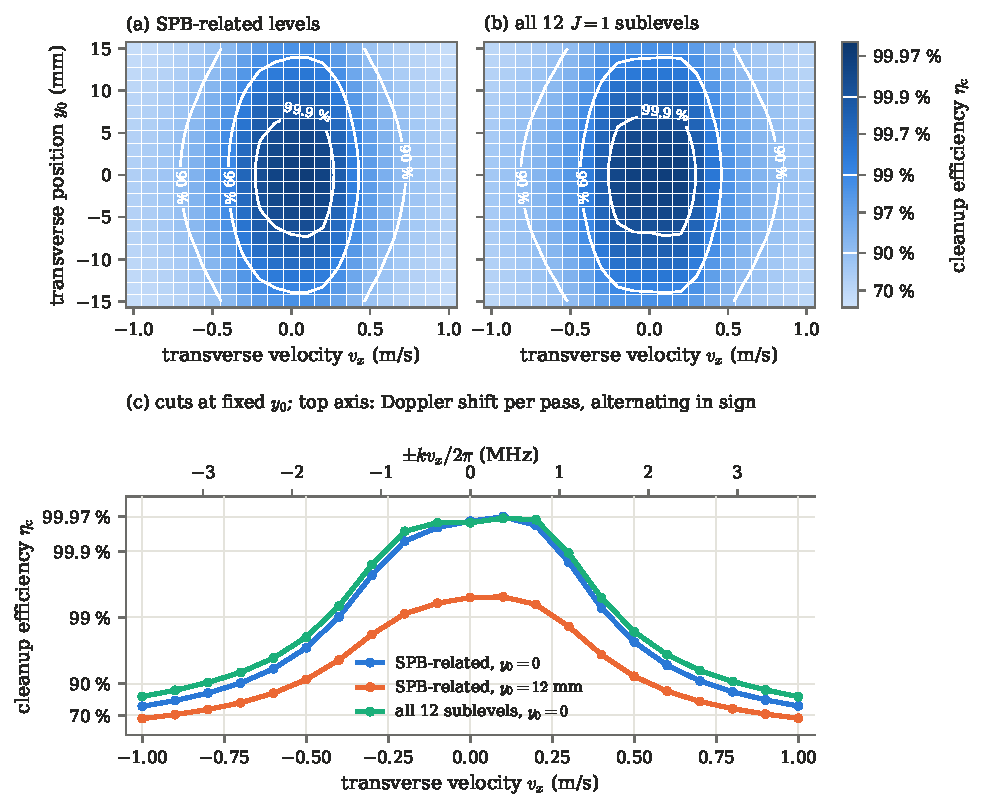
\includegraphics[width=\textwidth]{CU1_doppler_vx_y_map.pdf}
  \caption[CU1: cleanup versus transverse velocity and position]{CU1 cleanup versus transverse
  velocity $v_x$ and transverse position $y_0$ (\SI{80}{mW}, $+\SI{20.2}{MHz}$, \SI{4.8}{cm}
  beam, no EOM). (a) SPB-related initial state, (b) uniform 12-level initial state; logarithmic
  colour scale, white contours at 90, 99 and \SI{99.9}{\percent}; the grid was computed for
  $y_0\geq0$ and mirrored. (c) Cuts at fixed $y_0$; the top axis gives the Doppler shift per
  pass, whose sign alternates from pass to pass.}
  \label{fig:j1_doppler}
\end{figure}

\section{Choice of the set point}
\label{sec:j1_avg}

Averaged over a transverse velocity distribution, the on-axis optimum is not the best detuning.
The grids were averaged first over an assumed distribution ($v_x$ Gaussian with \SI{1.8}{m/s}
FWHM, cut at $|v_x|\leq\SI{1}{m/s}$; $y_0$ uniform within \SI{15}{mm}) and later over the beam
simulation within the detection acceptance (Sec.~\ref{sec:j1_present}). In both cases the average
has a minimum near the on-axis optimum and two maxima on either side of it, at $+\SI{19.0}{MHz}$
and at $+22.0$ to $+\SI{22.5}{MHz}$. The first is the better one: \SI{95.2}{\percent} against
\SI{93.0}{\percent} at $+\SI{20.2}{MHz}$ with the first assumption, and \SI{97.1}{\percent}
against \SI{95.5}{\percent} with the beam simulation (\SI{80}{mW}, \SI{4.8}{cm}). With the
\SI{3}{cm} beam the on-axis optimum moves to $+\SI{20.5}{MHz}$, but the mean in acceptance is again
best at $+\SI{19.0}{MHz}$ (\SI{98.66}{\percent}; second maximum \SI{98.43}{\percent} at
$+\SI{22.5}{MHz}$; script \code{scripts/cu1\_3cm\_scan.py}). \textbf{$+\SI{19.0}{MHz}$ was therefore
taken as the CU1 set point.} All of these averages assume $\sigma_{v_x}\leq\SI{0.76}{m/s}$; the best
detuning for the measured \SI{1.28}{m/s} has not been recomputed (Sec.~\ref{sec:exp_open}).

\paragraph{Broadening EOM.}
\label{sec:j1_eom}
Because the Doppler shift alternates in sign, it can only be covered by a broader laser spectrum.
A \SI{1.6}{MHz} phase EOM available in the laboratory, whose sideband spacing is close to
$\Gamma/2\pi$, was scanned in modulation depth and detuning (script
\code{scripts/cu1\_eom\_doppler\_scan.py}). The best setting, $\beta=1.5$ at $+\SI{20.0}{MHz}$,
raises the average over the first assumed distribution from 95.2 to \SI{96.1}{\percent}
(\SI{97.9}{\percent} against \SI{97.1}{\percent} with the beam simulation). The gain was judged too
small and the EOM was not adopted. With the measured, twice wider velocity distribution the balance
may be different; this has not been recomputed.

\section{Two groups of ground sublevels}
\label{sec:j1_traj19}

Figure~\ref{fig:j1_traj19} shows a trajectory on the axis at the set point, computed once for each
of the 12 starting sublevels (script \code{scripts/cu1\_trajectories.py}). In the field the 12
sublevels of $J=1$ form two groups \SI{2.4}{MHz} apart. The four mainly-$m_J=0$ levels, which
include the main ground state and the levels populated by AP1 (Sec.~\ref{sec:j1_ap1}), reach the
driven $|m_F'|=1$ components at $\delta/2\pi\approx+\SI{18.5}{MHz}$; the eight SPB-related,
mainly-$|m_J|=1$ levels only at $+20.7$ to $+\SI{20.9}{MHz}$. The latter group contains the two most
weakly coupled levels, $|F_1=\tfrac32,F=2,m_F=\pm2\rangle$ and $|F_1=\tfrac12,F=0\rangle$
($|M|^2=0.005$ and 0.003, against 0.014 to 0.106 for the other levels; relative units), which limit
the cleanup whenever the laser is off their resonance. At $+\SI{19.0}{MHz}$ with the \SI{4.8}{cm}
beam the laser is \SI{0.5}{MHz} from the upper group but 1.7--\SI{1.9}{MHz} below the lower one, and
9.4 and \SI{9.0}{\percent} remain in the two weak levels when the molecule starts there; every other
sublevel keeps 0.22--\SI{0.27}{\percent}. A molecule with $|v_x|\approx\SI{0.5}{m/s}$, however, sees
the laser \SI{1.84}{MHz} higher in half of the passes, on resonance with the lower group, and is
emptied completely. Since most molecules move transversely, a laser placed so that the
Doppler-shifted passes are resonant, at the cost of the molecules near rest, is better on average.
This is why the average over $v_x$ has its maxima on either side of the on-axis optimum.

\begin{figure}[htbp]
  \centering
  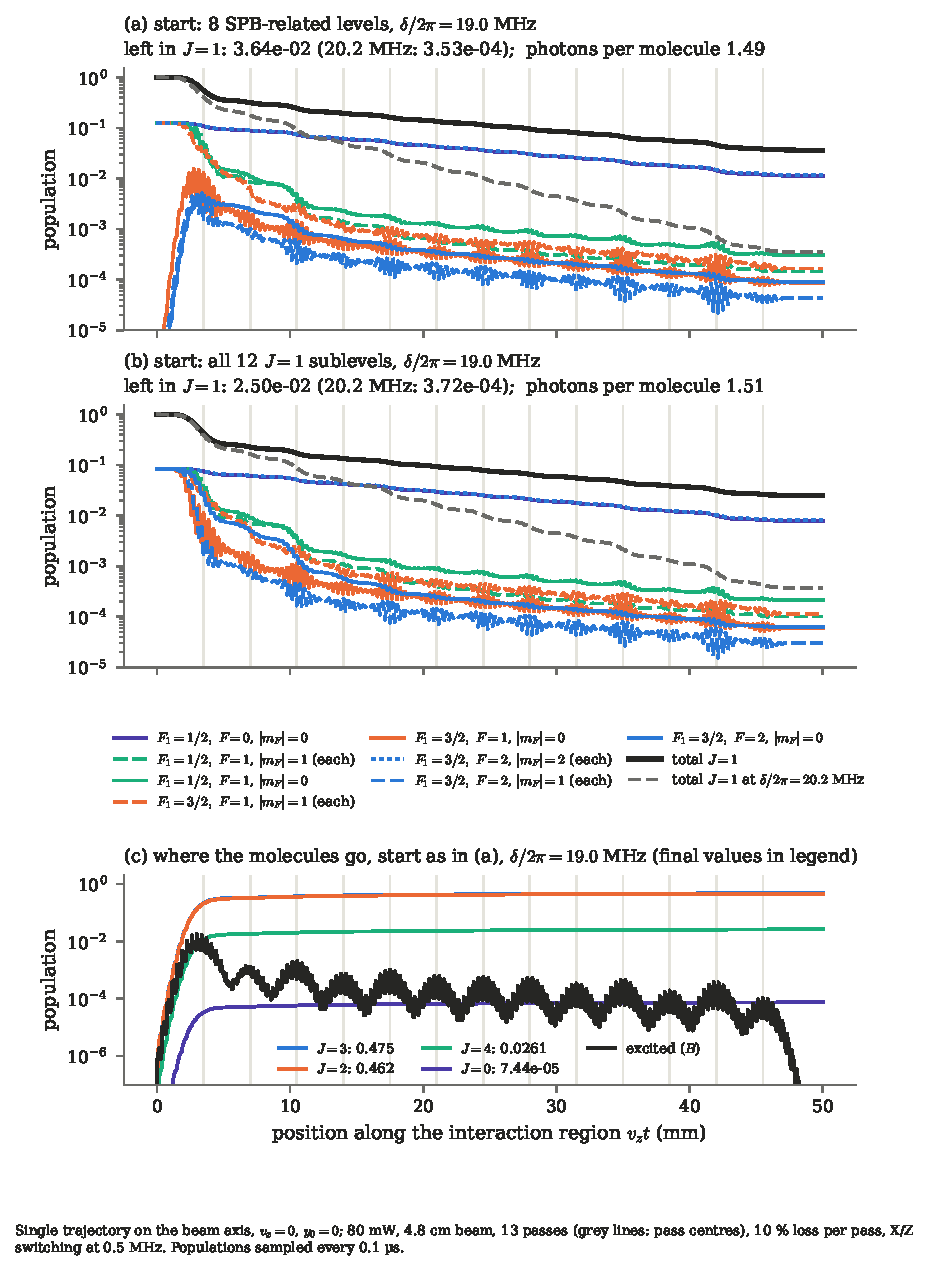
\includegraphics[width=\textwidth]{CU1_19MHz_J1_sublevels.pdf}
  \caption[CU1: sublevel populations at the set point]{CU1 at the set point $+\SI{19.0}{MHz}$
  on the axis ($v_x=0$, $y_0=0$), \SI{80}{mW}, \SI{4.8}{cm} beam, no EOM. (a) $J=1$ sublevel
  populations from the SPB-related start (one curve per $\pm m_F$ pair, equal by symmetry), with
  the total and, for comparison, the total at $+\SI{20.2}{MHz}$. (b) The same from the uniform
  12-level start. (c) Populations of the other rotational levels and of the excited state, start as
  in (a). Grey lines: pass centres.}
  \label{fig:j1_traj19}
\end{figure}

\section{Present and test conditions}
\label{sec:j1_present}

\paragraph{Mean in acceptance.} The results of this section are averaged over the transverse
distribution of a simulation of the lensed beam (\SI{25}{kV}): Gaussian $v_x$ with
$\sigma_{v_x}=\SI{0.65}{m/s}$ and Gaussian $y_0$ with $\sigma_y=\SI{10.95}{mm}$ at CU1, counted only
within the acceptance assumed for the detection laser, $|v_x|\leq\SI{1}{m/s}$ and
$|y_0|\leq\SI{8.5}{mm}$ (\emph{mean in acceptance}). The logarithm of the remaining population is
interpolated linearly in $y_0$ between grid points, and the cut is applied at the cleanup plane,
i.e.\ the transverse drift to the detector is neglected. The test showed that the detected $J=1$
molecules have a wider distribution, $\sigma_{v_x}=\SI{1.28}{m/s}$, extending beyond \SI{1}{m/s}
(Sec.~\ref{sec:exp_doppler}); the numbers of this section are predictions under the earlier
assumption.

\paragraph{Beam height and power.} The beam was first about \SI{3}{cm} high at \SI{80}{mW}; the test
was run with \SI{50}{mW} in a \SI{2}{cm} beam. Table~\ref{tab:j1_conditions} compares the two
(script \code{scripts/cu1\_conditions\_scan.py}, \code{centrex-tlf}~0.3.0 for the \SI{2}{cm}
runs). With \SI{50}{mW} and \SI{2}{cm} the best detuning is again $+\SI{19.0}{MHz}$, and the mean in
acceptance drops from 98.70 to \SI{96.52}{\percent}: the residual grows by a factor 2.7. The velocity
dependence hardly changes; the loss is at the edges of the acceptance (Fig.~\ref{fig:j1_present}).
The peak intensity is about the same (0.94 times that of the \SI{3}{cm} beam), but at
$y_0=\SI{8.5}{mm}$ the \SI{2}{cm} beam has \SI{24}{\percent} of its peak intensity against
\SI{53}{\percent} for the \SI{3}{cm} beam. At \SI{50}{mW} a \SI{3}{cm} beam reaches only
\SI{96.36}{\percent} on the axis, so the best height for \SI{50}{mW} lies between 2 and \SI{3}{cm}.

\begin{table}[htbp]
  \centering
  \caption[CU1 at the present and test conditions]{CU1 at the present (\SI{80}{mW},
  \SI{3}{cm}) and test (\SI{50}{mW}, \SI{2}{cm}) conditions, SPB-related start, no EOM. Left: detuning
  scan at \SI{50}{mW}, \SI{2}{cm} (coarse grid, run \code{detuning\_vx\_y\_cu1\_spb\_2cm\_50mW\_coarse}).
  Right: full maps at $+\SI{19.0}{MHz}$ (runs \code{doppler\_cu1\_spb\_3cm\_det19MHz} and
  \code{doppler\_cu1\_spb\_2cm\_50mW\_det19MHz}). Mean in acceptance as defined in the text.}
  \label{tab:j1_conditions}
  \small
  \begin{tabular}{ccc}
    \toprule
    $\delta/2\pi$ (MHz) & on axis & mean in acc. \\
    \midrule
    18.5 & \SI{96.32}{\percent} & \SI{95.27}{\percent} \\
    \textbf{19.0} & \SI{98.78}{\percent} & \textbf{\SI{96.52}{\percent}} \\
    19.5 & \SI{99.80}{\percent} & \SI{96.44}{\percent} \\
    20.5 & \SI{99.998}{\percent} & \SI{94.62}{\percent} \\
    22.0 & \SI{99.66}{\percent} & \SI{96.24}{\percent} \\
    \bottomrule
  \end{tabular}\hspace{6mm}
  \begin{tabular}{lcc}
    \toprule
    $+\SI{19.0}{MHz}$ & \SI{80}{mW}, \SI{3}{cm} & \SI{50}{mW}, \SI{2}{cm} \\
    \midrule
    on axis & \SI{99.01}{\percent} & \SI{98.78}{\percent} \\
    mean in acceptance & \textbf{\SI{98.70}{\percent}} & \textbf{\SI{96.52}{\percent}} \\
    $v_x=0$, $y_0=\SI{6}{mm}$ & \SI{97.47}{\percent} & \SI{93.21}{\percent} \\
    $v_x=0$, $y_0=\SI{9}{mm}$ & \SI{93.94}{\percent} & \SI{78.43}{\percent} \\
    $y_0=0$, $|v_x|=\SI{0.5}{m/s}$ & \SI{99.99}{\percent} & \SI{99.99}{\percent} \\
    $y_0=0$, $|v_x|=\SI{1}{m/s}$ & \SI{94.72}{\percent} & \SI{93.89}{\percent} \\
    \bottomrule
  \end{tabular}
\end{table}

\begin{figure}[htbp]
  \centering
  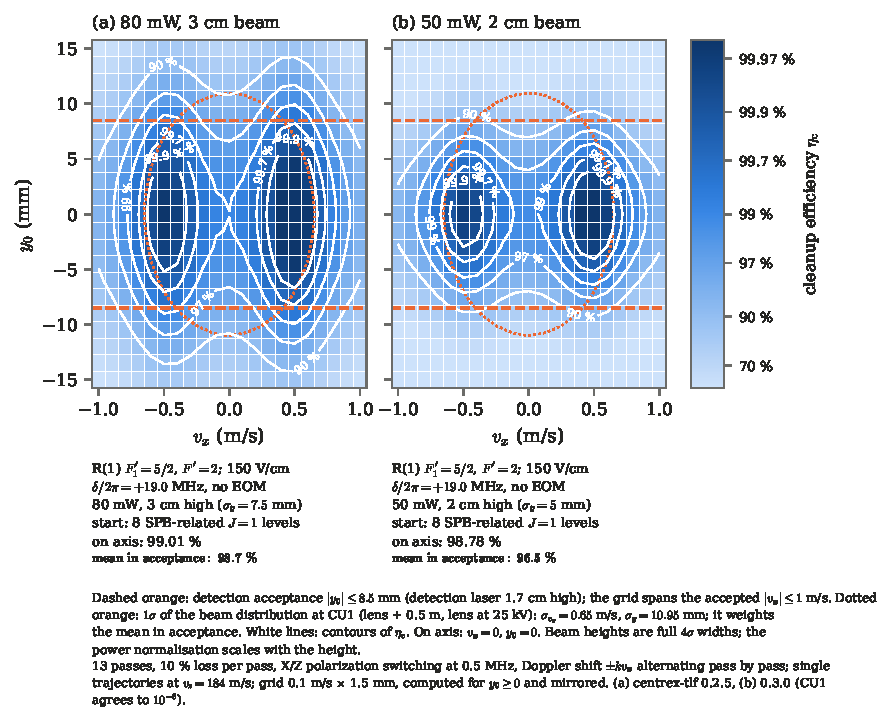
\includegraphics[width=0.92\textwidth]{cleanup_map_vx_y_CU1_2cm_50mW_vs_3cm_80mW.pdf}
  \caption[CU1 at the present and test conditions: cleanup versus $v_x$ and $y_0$]{CU1 cleanup
  versus transverse velocity and position at $+\SI{19.0}{MHz}$, no EOM, SPB-related start: (a) the
  present \SI{80}{mW}, \SI{3}{cm} beam, (b) the \SI{50}{mW}, \SI{2}{cm} beam of the test. Dashed lines:
  detection acceptance $|y_0|\leq\SI{8.5}{mm}$; dotted ellipse: $1\sigma$ of the beam distribution
  at CU1. The conditions and the mean in acceptance are given under each map.}
  \label{fig:j1_present}
\end{figure}

\section{Molecules from AP1}
\label{sec:j1_ap1}

In the test the $J=1$ molecules come from AP1, which populates the four mainly-$m_J=0$ levels of the
upper group (Sec.~\ref{sec:exp_detection}): the triplet $|F_1=\tfrac32,F=2,m_F=0,\pm1\rangle$ and
the singlet $|F_1=\tfrac32,F=1,m_F=0\rangle$. Each start was computed separately on the $(v_x,y_0)$
grid at the test conditions (\SI{50}{mW}, \SI{2}{cm}, $+\SI{19.0}{MHz}$; script
\code{scripts/cu1\_ap1\_start.py}, runs \code{doppler\_cu1\_ap1\_triplet\_2cm\_50mW\_det19MHz} and
\code{doppler\_cu1\_ap1\_singlet\_2cm\_50mW\_det19MHz}). Since the master equation is linear in
$\rho(0)$, the two can be combined with any weights.
\begin{itemize}
  \item \textbf{Triplet start:} \SI{98.65}{\percent} mean in acceptance (\SI{99.92}{\percent} on the
        axis). Two thirds of the \SI{1.35}{\percent} residual sit in $|F_1=\tfrac32,F=2,m_F=0\rangle$.
  \item \textbf{Singlet start:} \SI{99.68}{\percent}.
\end{itemize}
Both are better than the SPB-related start (\SI{96.52}{\percent}), because at $+\SI{19.0}{MHz}$ the
laser is close to the resonance of the upper group (Sec.~\ref{sec:j1_traj19}).

\paragraph{What R(1) $F'=3$ reads.} The detection line sees only $F=2$
(Sec.~\ref{sec:exp_detection}). With RC on P(2) $F'=2$ only the triplet is populated, and R(1)
reads the $F=2$ part of the triplet residual, \SI{1.15}{\percent} of the \SI{1.35}{\percent}. With RC
on $F'=1$ the singlet is the larger population (an estimated 0.64 triplet molecules per singlet
molecule). CU1 pumps
part of the singlet into $F=2$, where R(1) sees it, while the singlet itself is invisible with CU1
closed. The R(1) ratio is then
\begin{equation}
  r_{\mathrm R}=p_{t\to F=2}+\frac{N_s}{N_t}\,p_{s\to F=2},
  \label{eq:singlet_feed}
\end{equation}
with $p_{t\to F=2}$ and $p_{s\to F=2}$ the fractions of the triplet and singlet molecules found in
$F=2$ after CU1 and $N_s/N_t$ the singlet-to-triplet ratio. For $N_s/N_t=1/0.64$ the model gives
$r_{\mathrm R}=\SI{1.46}{\percent}$, of which \SI{0.31}{\percent} is singlet feed, i.e.\ about
\SI{27}{\percent} more than with the triplet alone. The triplet efficiency is therefore best
measured with RC on $F'=2$. These predictions use the pre-test assumptions; with the measured
velocity distribution the triplet residual is about \SI{3}{\percent} (Sec.~\ref{sec:exp_model}).

\section{Laser tilt}
\label{sec:j1_tilt}

If the CU1 laser is tilted by an angle $\theta$ from perpendicular, in the plane that contains the
molecular beam, every pass sees an additional Doppler shift $k_Lv_z\sin\theta/2\pi\approx
v_z\theta/\lambda$: \SI{0.68}{MHz} per mrad at \SI{184}{m/s}, \SI{0.53}{MHz} per mrad at
\SI{145}{m/s}. In the retro-reflecting two-prism multipass the return passes are antiparallel, so
this shift alternates in sign like the transverse one; the molecule sees $\pm k_L(v_x+v_z\theta)$.
A tilt is therefore equivalent to shifting the transverse velocity of every molecule by $v_z\theta$
(\SI{0.18}{m/s} per mrad at \SI{184}{m/s}), while the detection still selects on the true $v_x$, and
re-tuning the laser cannot remove it. A pointing error of the molecular beam, i.e.\ a mean $v_x\neq0$,
has the same effect. (With parallel passes the tilt would only be a common detuning, removed by
re-tuning.)

At \SI{50}{mW} and \SI{2}{cm} (Fig.~\ref{fig:j1_tilt}, script \code{scripts/cu1\_tilt\_scan.py}) the mean in acceptance falls from
\SI{96.52}{\percent} at $\theta=0$ to 95.85 and \SI{96.16}{\percent} at $\mp\SI{1}{mrad}$, 94.12 and
\SI{94.71}{\percent} at $\mp\SI{2}{mrad}$, and 91.49 and \SI{92.32}{\percent} at $\mp\SI{3}{mrad}$.
Re-tuning helps only beyond about \SI{3}{mrad}, by 0.5--\SI{1}{\percent}. \textbf{The tolerance is
$|\theta|\lesssim\SI{1}{mrad}$} (\SI{0.3}{mm} over \SI{30}{cm}), as for the \SI{80}{mW}, \SI{3}{cm}
beam, which loses 0.3--\SI{0.5}{\percent} at \SI{1}{mrad}. The tilt hurts because the set point relies
on the two velocity bands near $|v_x|=\SI{0.5}{m/s}$ that are cleaned best (Fig.~\ref{fig:j1_present});
a tilt slides the whole velocity distribution across them. In the test the laser was set
perpendicular to the molecular beam by overlapping the reflected beam with the incoming beam
(Sec.~\ref{sec:exp_progress}). These numbers use $\sigma_{v_x}=\SI{0.65}{m/s}$ and the SPB-related
start.

\begin{figure}[htbp]
  \centering
  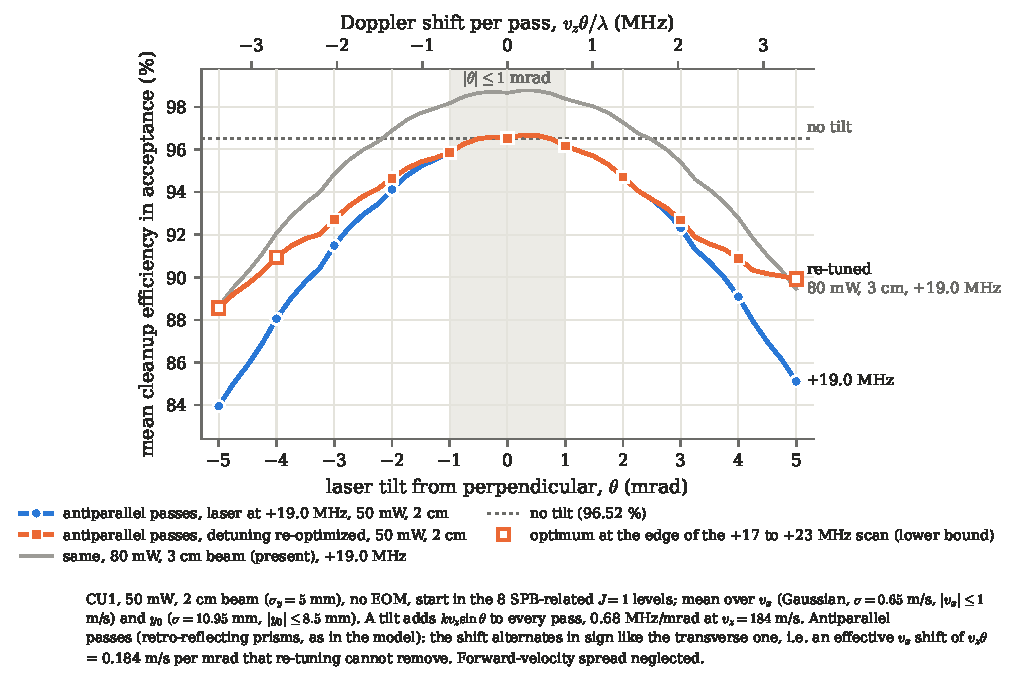
\includegraphics[width=0.92\textwidth]{CU1_laser_tilt_2cm_50mW.pdf}
  \caption[CU1: effect of a tilted laser]{CU1: mean cleanup in the detection acceptance versus the
  tilt of the laser from perpendicular, \SI{50}{mW}, \SI{2}{cm} beam, antiparallel passes, with the
  laser at $+\SI{19.0}{MHz}$ and with the detuning re-optimised; grey: the \SI{80}{mW}, \SI{3}{cm}
  beam at $+\SI{19.0}{MHz}$. Top axis: Doppler shift per pass at \SI{184}{m/s}. Open squares: the best
  detuning lies at the edge of the scanned range, so the value is a lower bound.}
  \label{fig:j1_tilt}
\end{figure}

\paragraph{Measuring the tilt with two passes.} With the first prism removed, the laser crosses the
molecular beam twice, in opposite directions, and a tilt splits the CU1 depletion line into two
peaks $2v_z\theta/\lambda$ apart (\SI{1.35}{MHz} per mrad at \SI{184}{m/s}), each broadened by the
transverse Doppler spread (FWHM \SI{8.7}{MHz} per m/s of $\sigma_{v_x}$). Figure~\ref{fig:j1_twopass}
shows the $F=2$ depletion seen by R(1) $F'=3$ computed for this configuration (two passes,
\SI{1}{mW}, on the beam axis, AP1 triplet start; script \code{scripts/cu1\_two\_pass\_test.py}). For
$\sigma_{v_x}=\SI{0.65}{m/s}$ a clear dip between the peaks appears only at about \SI{5}{mrad}
(\SI{20}{\percent} deep); for a collimated beam with $\sigma_{v_x}=\SI{0.2}{m/s}$ it appears from
\SI{2}{mrad} (\SI{5}{\percent}) and is \SI{35}{\percent} deep at \SI{3}{mrad}. The laser power must stay
at 0.3--\SI{1}{mW}: at \SI{3}{mW} the line saturates and shows a small dip even at $\theta=0$. With the
measured $\sigma_{v_x}=\SI{1.28}{m/s}$ (FWHM \SI{11}{MHz} per pass; splitting \SI{1.07}{MHz} per mrad at
\SI{145}{m/s}) the two peaks would separate only beyond about \SI{10}{mrad}. Comparing the centres of
single-pass spectra taken in the two directions, which differ by $2v_z\theta/\lambda$, is the more
sensitive test.

\begin{figure}[htbp]
  \centering
  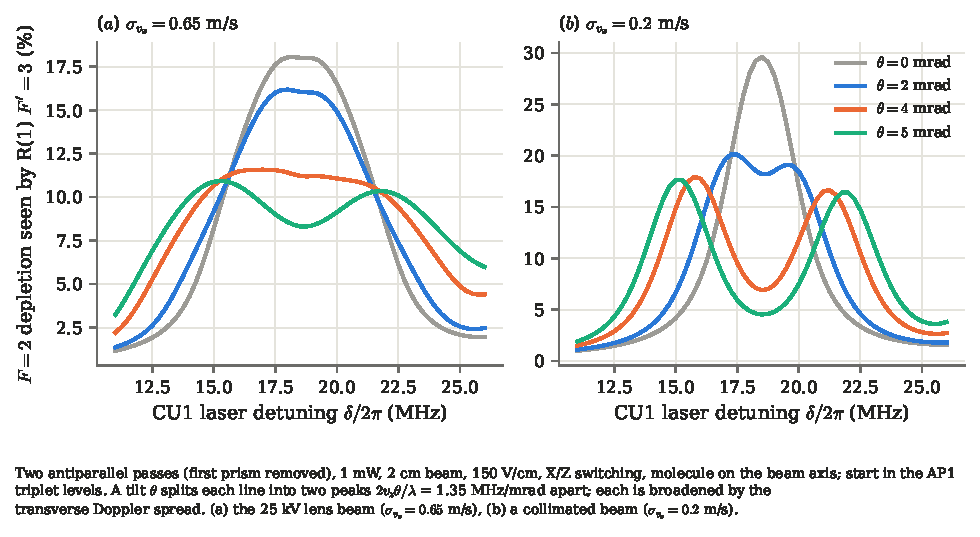
\includegraphics[width=\textwidth]{CU1_two_pass_tilt_test.pdf}
  \caption[CU1: two-pass test of the laser tilt]{Two-pass test of the CU1 laser tilt: $F=2$
  depletion seen by R(1) $F'=3$ versus CU1 detuning for tilts of 0, 2, 4 and \SI{5}{mrad} (first prism
  removed, \SI{1}{mW}, \SI{2}{cm} beam, \SI{150}{V/cm}, X/Z switching, molecule on the beam axis, AP1
  triplet start, \SI{184}{m/s}). (a) $\sigma_{v_x}=\SI{0.65}{m/s}$, (b) $\sigma_{v_x}=\SI{0.2}{m/s}$.}
  \label{fig:j1_twopass}
\end{figure}

% =====================================================================
\chapter{CU1 test on the SPB setup}
\label{ch:j1_exp}

CU1 was tested on the SPB setup between 2026-10-16 and 2026-10-21~\cite{CU1GroupMeeting2026}.
The best result is a cleanup efficiency of \SI{97.4(2)}{\percent} for the detected $J=1$, $F=2$
molecules at \SI{50}{mW} (Sec.~\ref{sec:exp_final}). The power dependence and the transverse
velocity, both measured in the same setup, show that the residual comes from molecules with
$|v_x|\gtrsim\SI{1}{m/s}$, which the wide acceptance of the test detection admits. With the measured
velocity distribution the CU1 model of Chapter~\ref{ch:j1} reproduces the power dependence with a
pass loss of a few per cent, where the earlier distribution required the power to be scaled down by
a factor of four (Sec.~\ref{sec:exp_model}). The figures of this chapter are the analysis figures of
the test; the line positions are collected in Appendix~\ref{app:exp_lines}.

\section{Setup}
\label{sec:exp_setup}

Table~\ref{tab:exp_config} lists the configuration. Two coordinate frames are used, as in
Sec.~\ref{sec:laser}: the laboratory frame with $Z$ along the beamline, $X$ horizontal and $Y$
vertical; and the laser frame, with $z$ along the CU1 field ($=Y$) and $x$ horizontal and
perpendicular to the laser propagation ($=Z$). CU1 and the detection laser both propagate along $X$,
so the Doppler shift is set by $v_x$, the velocity along $X$. The electrostatic lens hardly acts on the
$J=1$ molecules from AP1, which therefore follow nearly straight trajectories from the cell. The
detection, \SI{3.15}{m} from the cell, collects molecules out to $|X|\approx\SI{25}{mm}$ and beyond,
i.e.\ with $|v_x|$ up to about 1.2--\SI{1.7}{m/s}. In the final experiment the detection is \SI{8}{m} downstream behind
a \SI{2}{cm} aperture and accepts only $|v_x|\leq\SI{0.22}{m/s}$.

\begin{table}[htbp]
  \centering
  \caption[Configuration of the CU1 test]{Configuration of the CU1 test on the SPB setup. Powers are
  at the output of the doubling cavity. Distances from the cell.}
  \label{tab:exp_config}
  \small
  \begin{tabularx}{\textwidth}{lL}
    \toprule
    geometry & cell $\to$ RC $\to$ SPA $\to$ electrostatic lens (about \SI{2.0}{m}; its \SI{1.75}{in}
      bore is the aperture) $\to$ CU1 (\SI{2.5}{m}) $\to$ detection Det2 (\SI{3.15}{m}) \\
    upstream & RC on P(2) $F_1'=3/2$, $F'=2$ (from 10-19; $F'=1$ before and for the final Q(1) run), with
      the RC microwaves; lens $\pm\SI{24.7}{kV}$; SPA AP1 on, AP2 off; SPB high voltage on, SPB microwaves
      off \\
    CU1 & R(1) $F_1'=5/2$, $F'=2$ in \SI{156}{V/cm} (electrodes $\pm\SI{1250}{V}$); \SI{50}{mW} (about
      \SI{45}{mW} at the multipass entrance; minimum \SI{13}{mW}); \SI{2}{cm} high; two-prism multipass,
      about 17 passes after realignment (13 before); polarization EOM on (X/Z switching) \\
    shutter & SR475 in the CU1 beam, toggled on every ablation shot (\SI{16.67}{Hz}); state read from a
      photodiode \\
    detection & Det2 on R(1) $F_1'=5/2$, $F'=3$ (Q(1) $F_1'=1/2$, $F'=1$ in Sec.~\ref{sec:exp_q1});
      \SI{1.5}{cm} high (\SI{1}{cm} before 10-19); along $X$, parallel to CU1; polarization along the
      beamline (laser $x$), perpendicular to the CU1 field; PMT fluorescence normalised by absorption \\
    forward velocity & 141--\SI{145}{m/s} (absorption-peak method), 154--\SI{157}{m/s} (travel-time fit);
      the model uses \SI{145}{m/s} \\
    \bottomrule
  \end{tabularx}
\end{table}

\section{Detection}
\label{sec:exp_detection}

Two detection lines were used.
\begin{itemize}
  \item \textbf{R(1) $F_1'=5/2$, $F'=3$} couples only the five sublevels of $F_1=3/2$, $F=2$, and
        within $J=1$ its excited level decays only back to $F=2$. There is no dark state, so as long
        as the probe pumps every $F=2$ molecule out completely, each gives the same signal, and the
        ratio of two R(1) signals is the ratio of the $F=2$ populations. The other $J=1$ levels,
        among them the singlet $|F_1=\tfrac32,F=1,m_F=0\rangle$, are not seen.
  \item \textbf{Q(1) $F_1'=1/2$, $F'=1$} couples all 12 sublevels of $J=1$. With 12 ground and only 3
        excited sublevels, however, the molecules are pumped into dark superpositions during the
        detection, so the signal per molecule depends on the sublevel. The Q(1) ratio is therefore not
        the remaining fraction of the whole $J=1$ level, and the Q(1) and R(1) signals are not compared
        quantitatively.
\end{itemize}
AP1 transfers all four $J=0$ hyperfine sublevels to the four mainly-$m_J=0$ levels of $J=1$: the
three triplet levels $|F_1=\tfrac32,F=2,m_F=0,\pm1\rangle$ and the singlet
$|F_1=\tfrac32,F=1,m_F=0\rangle$~\cite{Grasdijk2025AP}. RC on P(2) $F'=2$ enhances $J=0$, $F=1$ and
therefore the triplet, which R(1) sees; RC on $F'=1$ enhances $J=0$, $F=0$ and therefore the singlet,
with an estimated 0.64 triplet molecules per singlet molecule (from the RC scan of
Fig.~\ref{fig:exp_rc}). With RC on $F'=1$
the R(1) ratio also contains singlet molecules that CU1 pumps into $F=2$ (Eq.~\eqref{eq:singlet_feed}).

\section{Measurement method}
\label{sec:exp_method}

The shutter alternates between open and closed on consecutive ablation shots. A burst of 20 shots on
one target spot contains 10 open and 10 closed shots, and the state of every shot is read from the
photodiode. Open and closed shots share the ablation spot, the source and the absorption drifts,
which cancel in their ratio, and the closed shots are a true reference with CU1 blocked. Before the
shutter, an off-resonant CU1 frequency served as the reference; it lay on the wings of the CU1
spectrum (Fig.~\ref{fig:exp_spectrum}) and biased the result. The remaining fraction and the
efficiency are
\begin{equation}
  r=A_{\mathrm{open}}/A_{\mathrm{closed}},\qquad \etac=1-r,
\end{equation}
where $A$ is the amplitude of a fit of the mean open- and closed-shot traces to the smoothed mean
closed-shot trace (template) plus a linear baseline. The baseline absorbs the drift of the CU1
scattered light on the PMT (about \SI{1.7}{mV}). The integrals over a fixed window (12.8--\SI{41.8}{ms}
after the ablation trigger) and over the peak (18--\SI{30}{ms}) are cross-checks. Uncertainties are
\SI{68}{\percent} intervals from a bootstrap over bursts, cross-checked with a block bootstrap. Line,
frequency and Doppler scans are normalised by the absorption signal.

\section{Frequency, alignment and progress}
\label{sec:exp_progress}

\paragraph{CU1 spectrum.} The first CU1 spectra (10-16, before the shutter; Fig.~\ref{fig:exp_spectrum})
put the main pair \SI{9.1}{MHz} (IR) above the transition-finder value; this defines the detuning axis
below (UV detuning $=4\times$ IR). The opposite-parity component appears at $+\SI{61}{MHz}$.

\paragraph{Progress at the set point.} Figure~\ref{fig:exp_progress} shows how the remaining fraction
at \SI{50}{mW} fell from 0.099 (10-18, first shutter run) to 0.026 (10-19). Three alignment changes and
one change of the RC line contributed:
\begin{enumerate}[itemsep=0pt]
  \item a cross alignment laser put the CU1 beam, the detection beam and the chamber centre at the same
        height;
  \item the number of passes was increased from 13 to about 17;
  \item the reflected CU1 beam was overlapped with the incoming beam, so that the laser is
        perpendicular to the molecular beam (Sec.~\ref{sec:j1_tilt});
  \item RC was moved from P(2) $F'=1$ to $F'=2$ (0.064 to 0.047). Part of this step is expected from the
        singlet feed of Eq.~\eqref{eq:singlet_feed}, which is absent with RC on $F'=2$.
\end{enumerate}

\paragraph{Frequency dependence.} The optimum lies at NLTL 2465.5--\SI{2466.0}{MHz}
(Fig.~\ref{fig:exp_freq}a), i.e.\ $+14$ to $+\SI{16}{MHz}$ (UV) from the main pair, 4--\SI{6}{MHz} below
the predicted set point (NLTL $\approx\SI{2464.5}{MHz}$). The offset is not understood
(Sec.~\ref{sec:exp_open}). RC on $F'=2$ and the realigned multipass lower the whole curve; enlarging
the probe from 1 to \SI{1.5}{cm} leaves the remaining fraction unchanged and increases the signal by a
factor 1.58. The multipass alignment matters (Fig.~\ref{fig:exp_freq}b): alignment A (more passes,
some clipped) and C (realigned, about 17 passes) beat B (13 clean passes). Alignments are hard to
reproduce, so each attempt was scored by a quick check of 30--40 bursts ($\pm0.005$).

\begin{figure}[htbp]
  \centering
  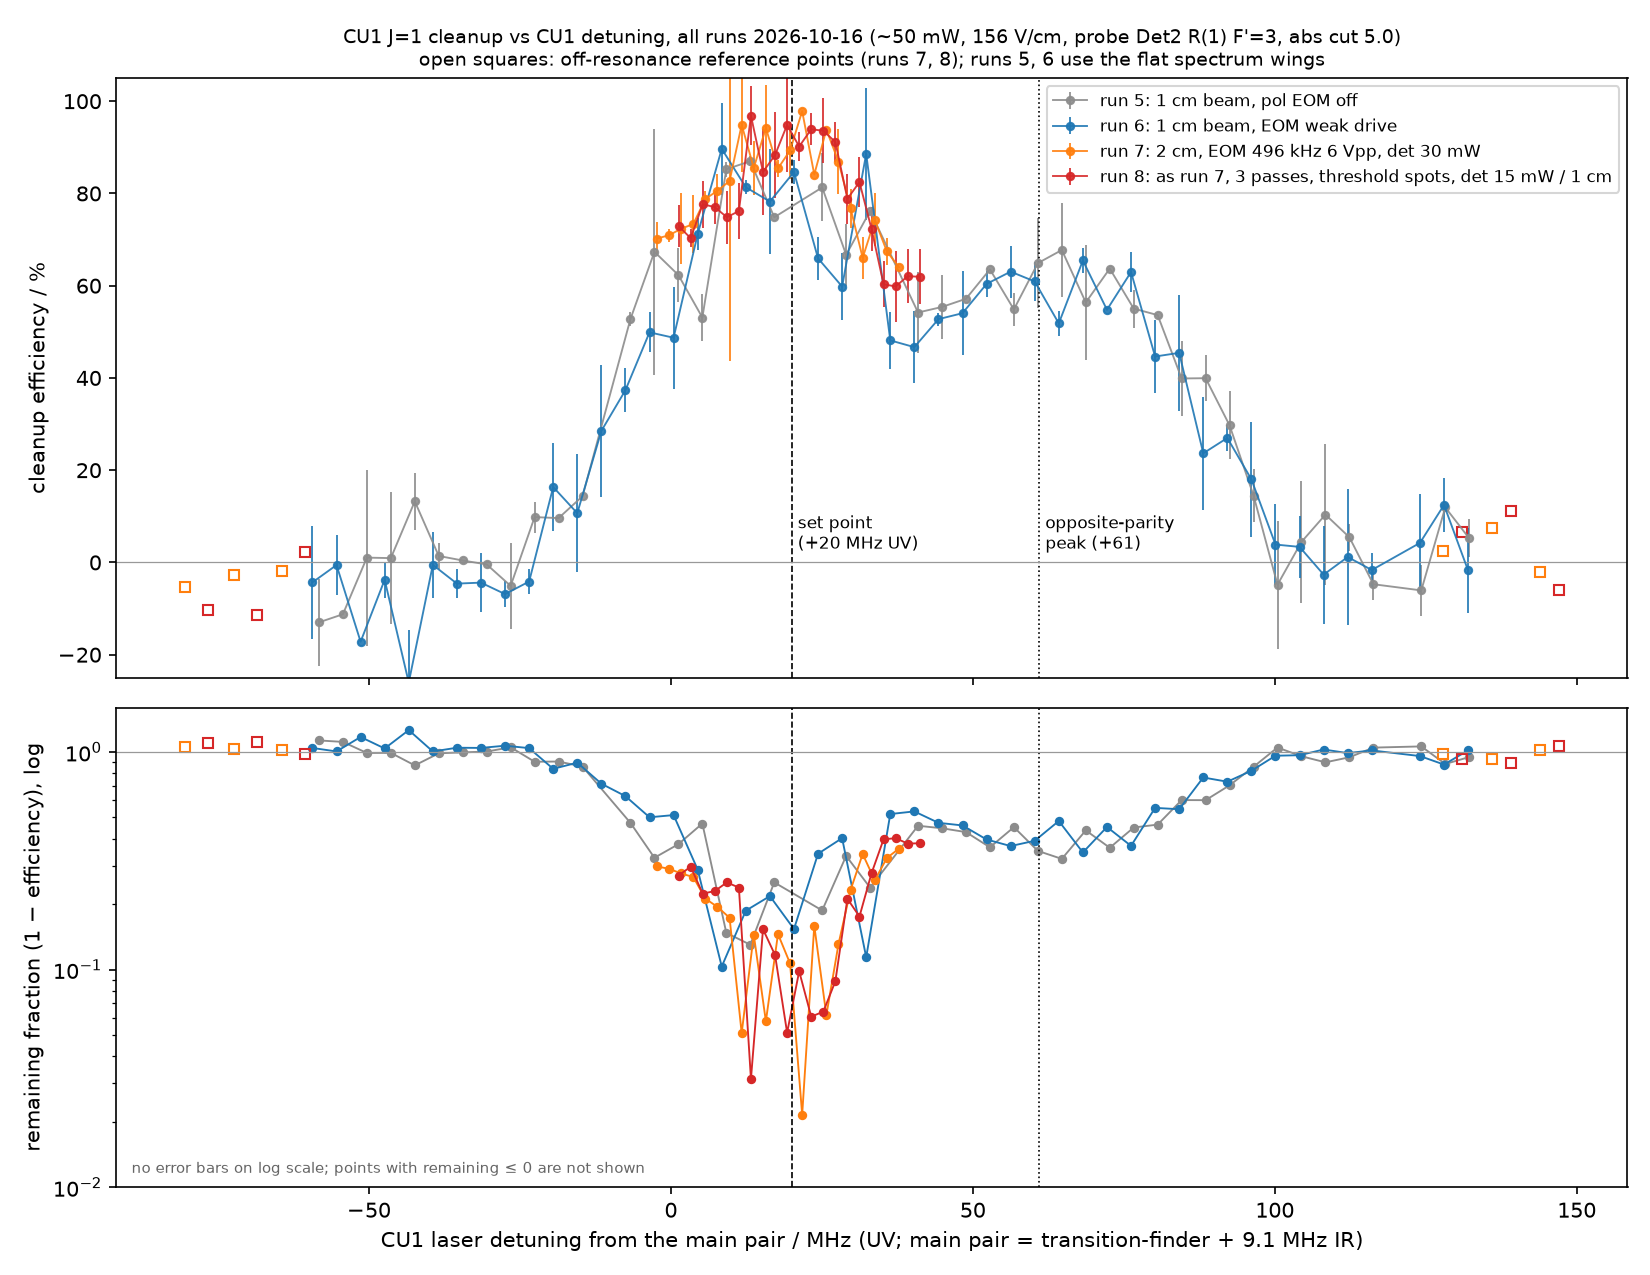
\includegraphics[width=0.8\textwidth]{experiment/exp_03_cu1_spectrum_2026-10-16.png}
  \caption[CU1 test: first CU1 spectra]{CU1 test: cleanup efficiency (top) and remaining fraction
  (bottom) versus CU1 detuning from the main pair, all runs of 10-16, before the shutter (about
  \SI{50}{mW}, \SI{156}{V/cm}, detection R(1) $F'=3$). Open squares: off-resonance reference points.
  Vertical lines: set point and opposite-parity peak.}
  \label{fig:exp_spectrum}
\end{figure}

\begin{figure}[htbp]
  \centering
  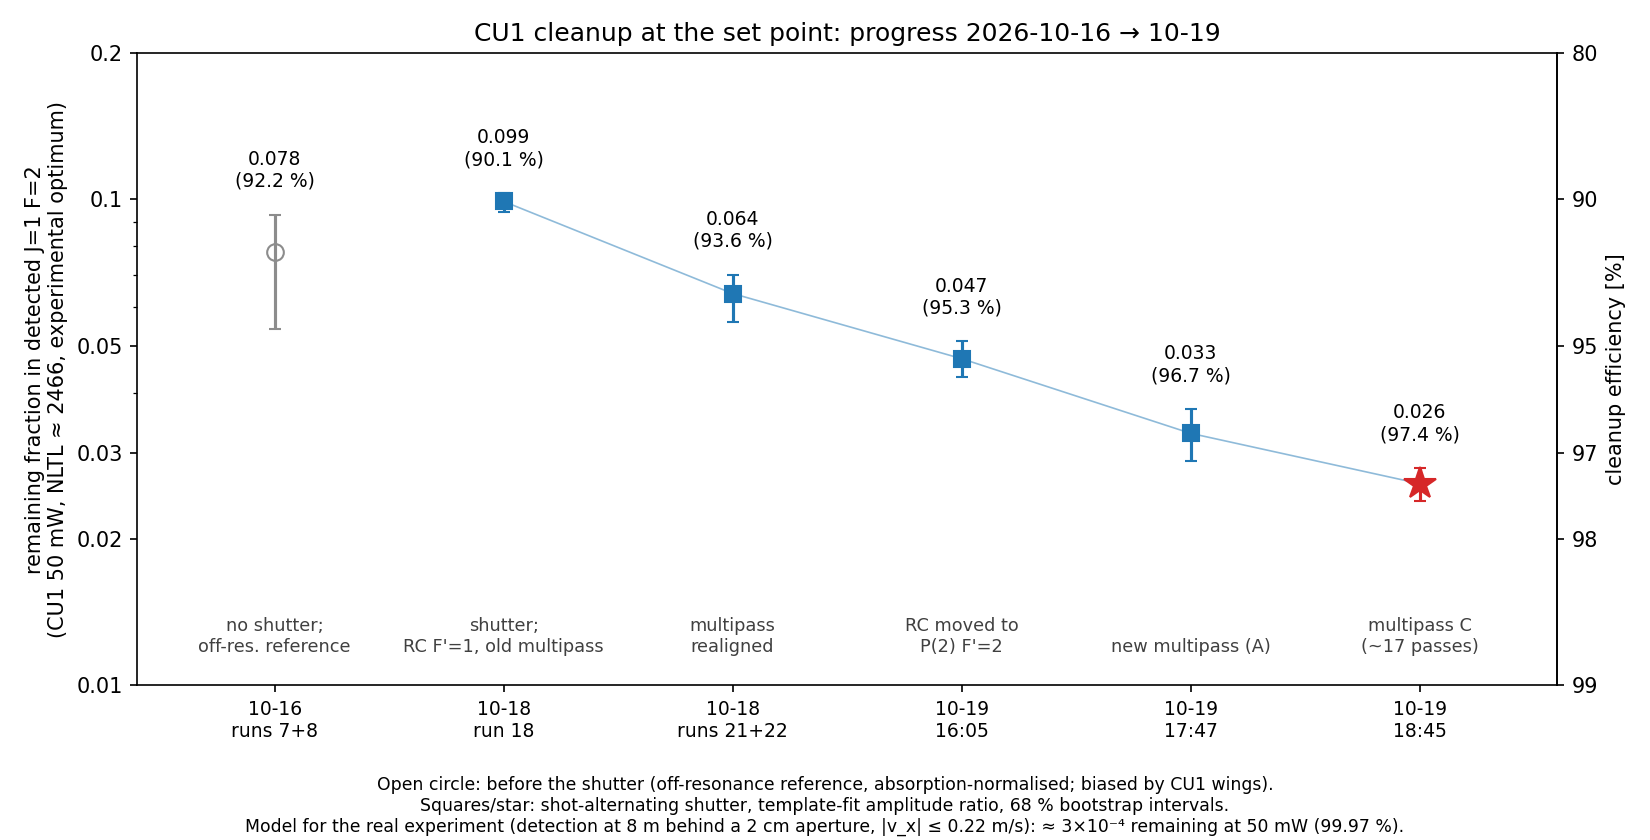
\includegraphics[width=\textwidth]{experiment/exp_04_progress_set_point.png}
  \caption[CU1 test: progress at the set point]{CU1 test: remaining fraction of the detected $J=1$,
  $F=2$ population at the set point (\SI{50}{mW}, NLTL $\approx2466$) from 10-16 to 10-19, with the
  change made before each point. Open circle: before the shutter (off-resonance reference, biased by
  the CU1 wings). Squares and star: shot-alternating shutter, template fit, \SI{68}{\percent} bootstrap
  intervals.}
  \label{fig:exp_progress}
\end{figure}

\begin{figure}[htbp]
  \centering
  \begin{subfigure}{0.7\textwidth}
    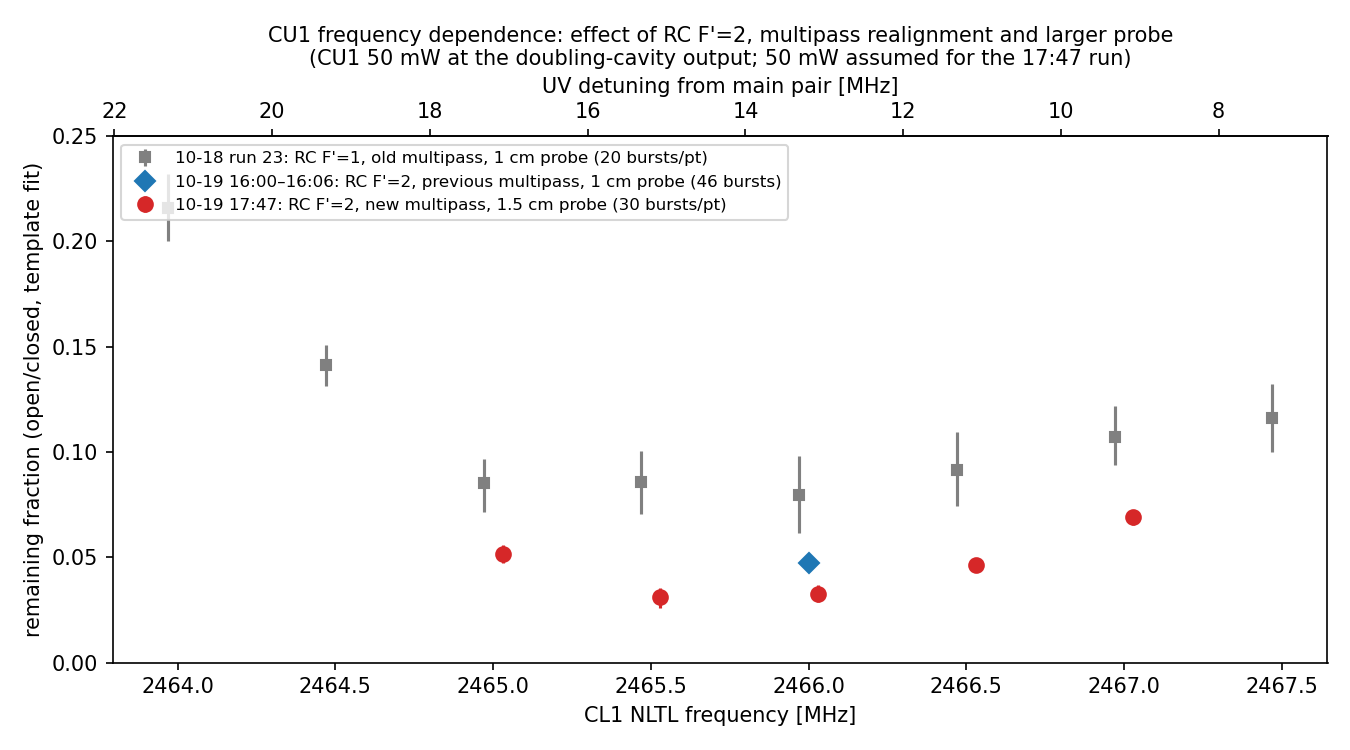
\includegraphics[width=\textwidth]{experiment/exp_05_freqscan_RC_F2_multipass.png}
    \caption{}
  \end{subfigure}\\[2mm]
  \begin{subfigure}{0.7\textwidth}
    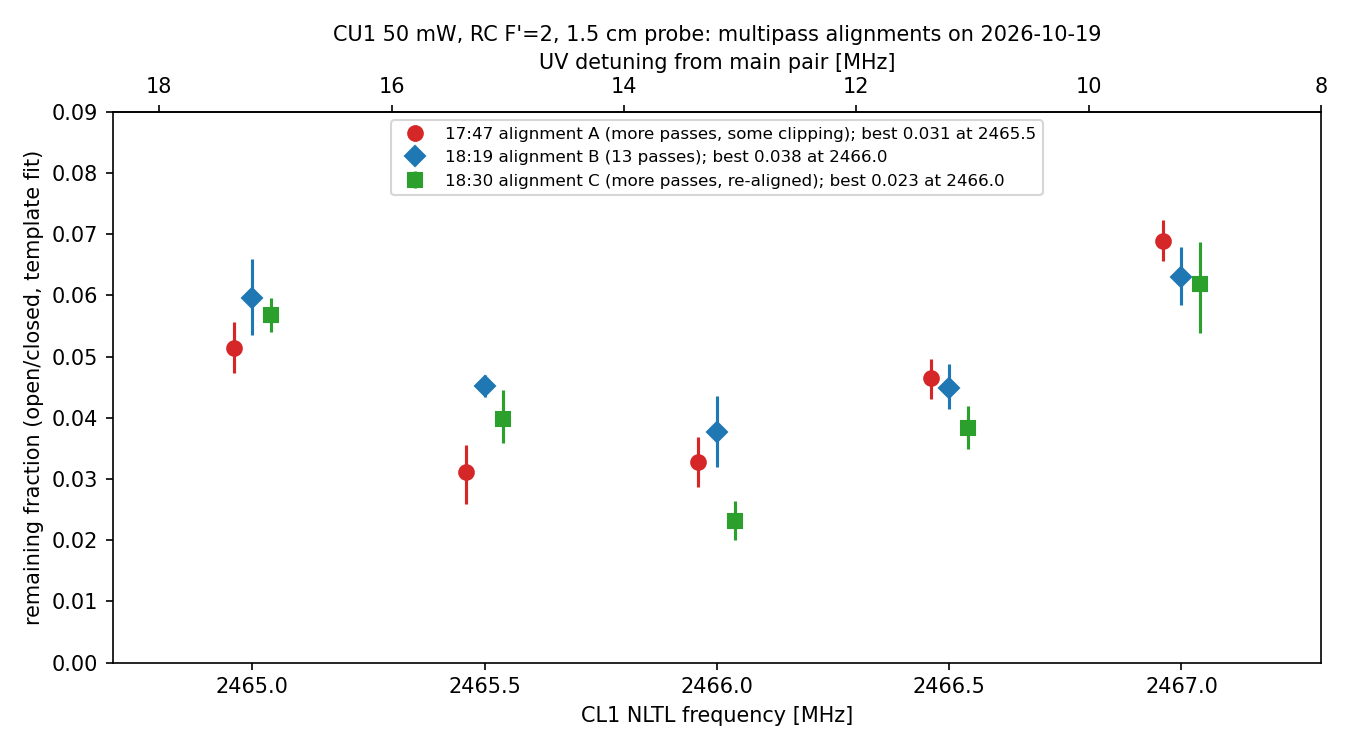
\includegraphics[width=\textwidth]{experiment/exp_06_multipass_alignments_ABC.png}
    \caption{}
  \end{subfigure}
  \caption[CU1 test: frequency dependence and multipass alignment]{CU1 test: remaining fraction versus
  CU1 frequency (NLTL; top axis: UV detuning from the main pair) at \SI{50}{mW}. (a) Effect of RC on
  $F'=2$, the realigned multipass and the larger probe. (b) Multipass alignments A, B and C on 10-19,
  RC on $F'=2$, \SI{1.5}{cm} probe.}
  \label{fig:exp_freq}
\end{figure}

\section{Final result}
\label{sec:exp_final}

The final run (10-19, 18:45--18:48; Fig.~\ref{fig:exp_final}) used alignment C at NLTL
\SI{2466.0}{MHz} and \SI{50}{mW}, with RC on $F'=2$: 100 bursts of 20 shots (1000 open and 1000 closed)
on 20 target spots in \SI{2.7}{min}. The template fit gives
\begin{equation*}
  r=0.026\ [0.024,0.028],\qquad \etac=\SI{97.4(2)}{\percent},
\end{equation*}
with $[0.024,0.029]$ from the block bootstrap and $0.024\ [0.019,0.029]$ from the window integral. On
10-21 the best point had moved to NLTL \SI{2465.5}{MHz}, where the remaining fraction was 0.025--0.032
(\SI{96.8}{\percent} at \SI{50}{mW} in the power series of Sec.~\ref{sec:exp_model}).

\begin{figure}[htbp]
  \centering
  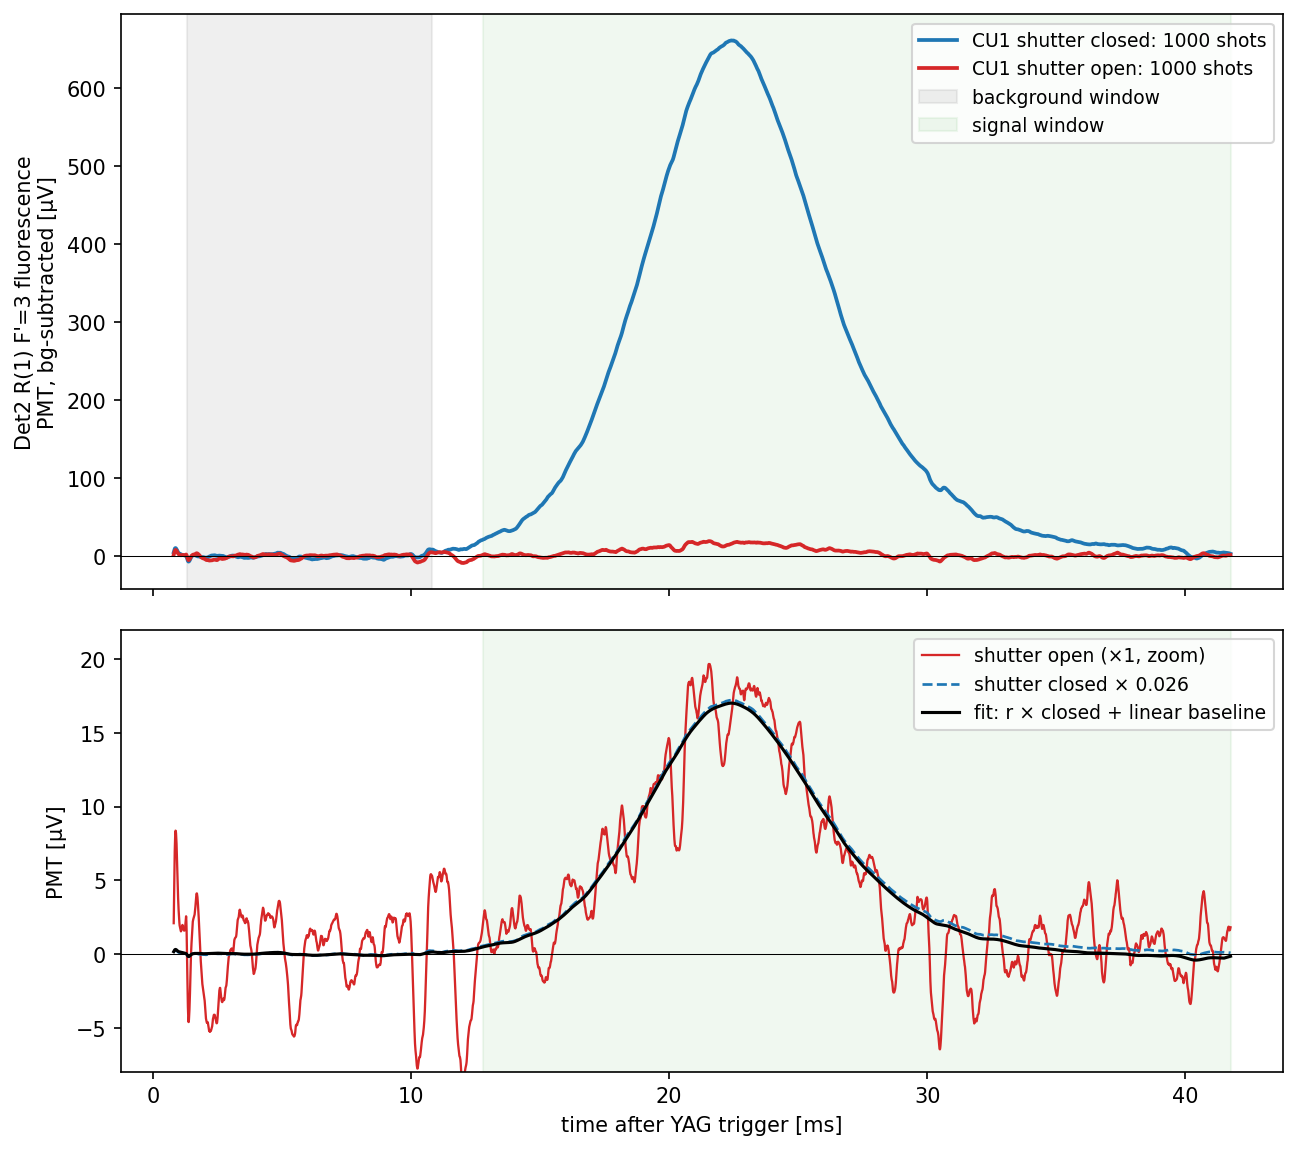
\includegraphics[width=0.72\textwidth]{experiment/exp_08_final_result.png}
  \caption[CU1 test: final result]{CU1 test, final run: mean PMT traces with the CU1 shutter closed
  and open (top) and, enlarged, the open-shutter trace with the fit $r\times$closed${}+{}$linear
  baseline (bottom). Grey: background window; green: signal window.}
  \label{fig:exp_final}
\end{figure}

\section{Power dependence}
\label{sec:exp_power}

With the 13-pass alignment (10-19, NLTL \SI{2466.0}{MHz}, 40 bursts per power) the remaining fraction
was 0.199, 0.183, 0.089, 0.081 and 0.056 at 13, 15, 30, 40 and \SI{50}{mW} (Fig.~\ref{fig:exp_power}).
A fit of $r=\exp(-kP^a)$ gives $a=0.45\pm0.03$. For a homogeneous ensemble the optical depth $-\ln r$
grows linearly with the power, $a=1$; the slow, square-root-like growth points to an inhomogeneous
distribution of Doppler shifts, not to a hard floor. With alignment C at NLTL \SI{2465.5}{MHz} (10-21,
separate quick checks of 40 bursts) the remaining fraction was 0.150, 0.063, 0.045 and 0.032 at 13, 30,
40 and \SI{50}{mW}, again with $a=0.44$.

\begin{figure}[htbp]
  \centering
  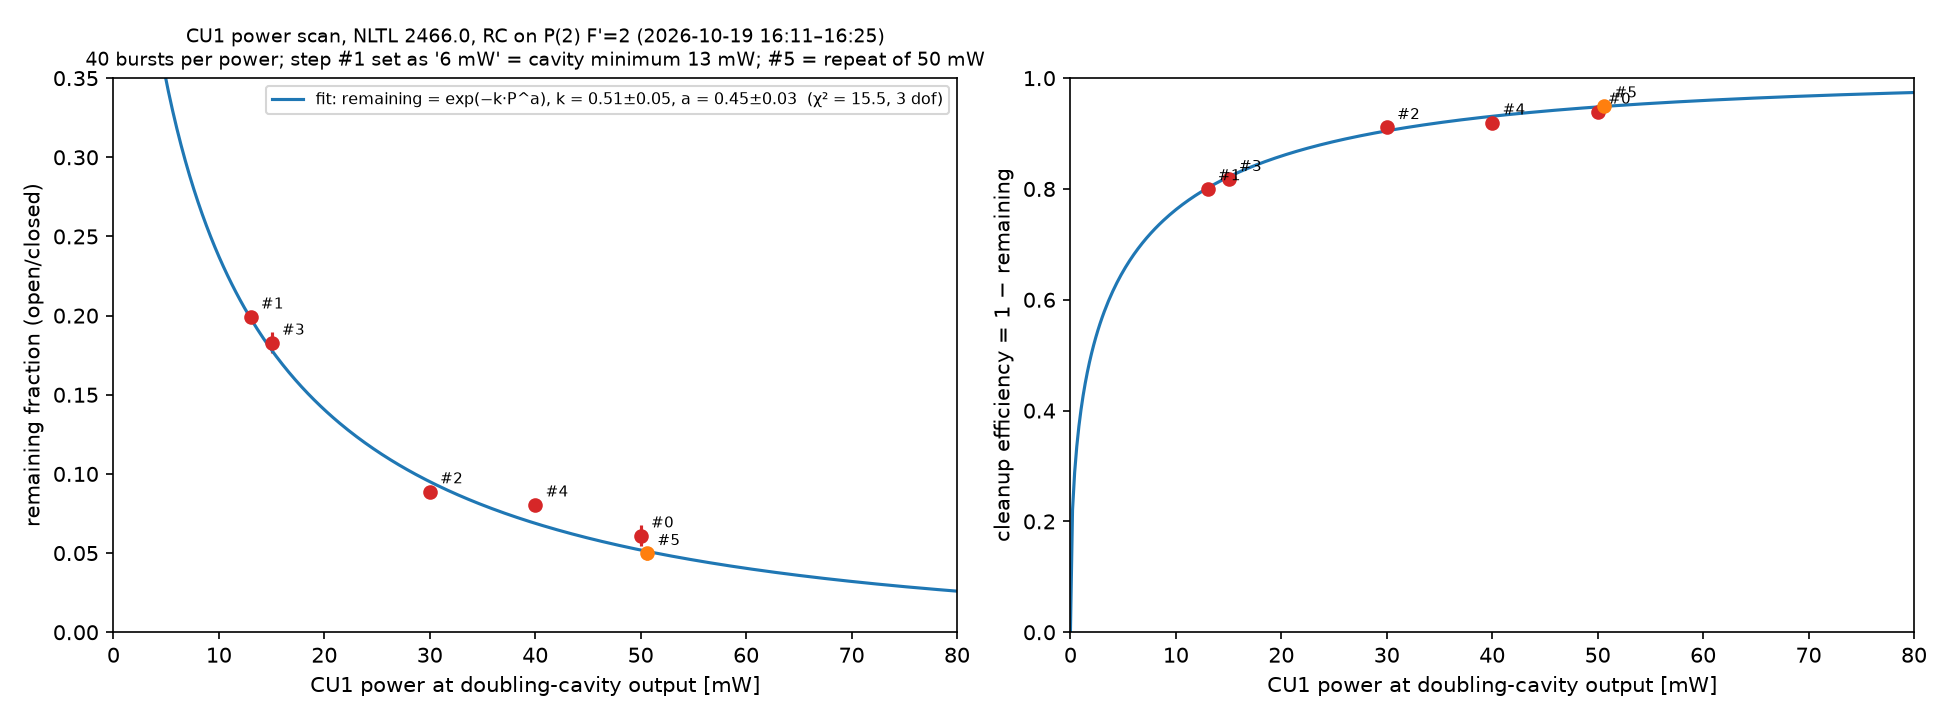
\includegraphics[width=\textwidth]{experiment/exp_07_power_scan_2026-10-19.png}
  \caption[CU1 test: power dependence]{CU1 test: remaining fraction (left) and efficiency (right) versus
  CU1 power at the doubling-cavity output, 13-pass alignment, NLTL \SI{2466.0}{MHz}, RC on $F'=2$, 40
  bursts per power, with the fit $r=\exp(-kP^a)$.}
  \label{fig:exp_power}
\end{figure}

\section{Transverse velocity of the detected molecules}
\label{sec:exp_doppler}

With CU1 off, the detection laser was scanned across R(1) $F'=3$ at 400 and \SI{100}{\micro W}
(10-20, Fig.~\ref{fig:exp_doppler}). Since it propagates along $X$, parallel to CU1, the line shape is
the $v_x$ distribution of the detected molecules. A Voigt fit with the Lorentzian width fixed to the
natural width (\SI{0.4}{MHz} in the IR) gives $\sigma_G=1.19\pm0.01$ and \SI{1.18(3)}{MHz} (IR), i.e.
\begin{equation*}
  \sigma_{v_x}=\SI{1.29(1)}{m/s}\ (\SI{400}{\micro W}),\qquad \SI{1.28(3)}{m/s}\ (\SI{100}{\micro W}),
\end{equation*}
with \SI{1}{MHz} (IR) corresponding to \SI{1.087}{m/s}. The two powers agree, so there is no visible
saturation broadening, and a simulation of the $J=1$ beam through the lens (\SI{25}{kV},
\SI{145}{m/s}) gives \SI{1.37}{m/s}. \textbf{The detected $J=1$ molecules have $\sigma_{v_x}=\SI{1.28}{m/s}$},
twice the \SI{0.65}{m/s} of the lensed $J=2$ beam assumed in Chapter~\ref{ch:j1}.

\begin{figure}[htbp]
  \centering
  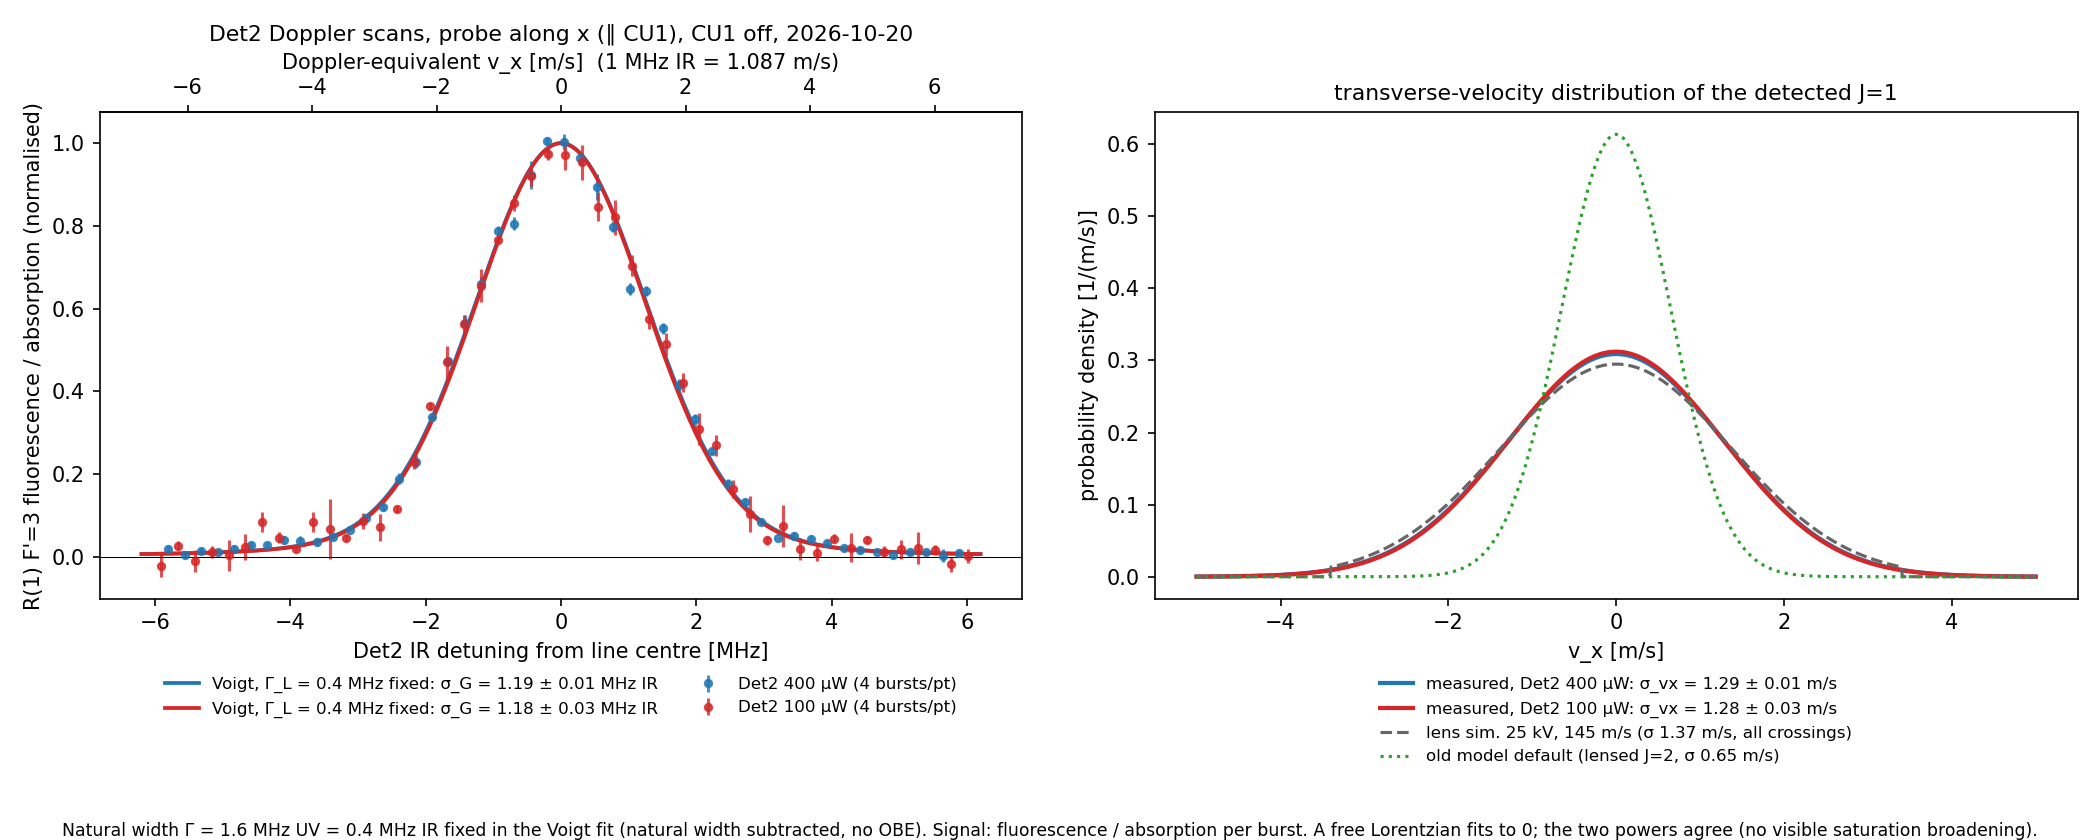
\includegraphics[width=\textwidth]{experiment/exp_09_doppler_vx_distribution.png}
  \caption[CU1 test: transverse velocity of the detected $J=1$ molecules]{CU1 test: Doppler scan of
  R(1) $F'=3$ with the detection laser along $X$, CU1 off. Left: fluorescence over absorption versus IR
  detuning (top axis: equivalent $v_x$) with Voigt fits ($\Gamma_L=\SI{0.4}{MHz}$ IR fixed). Right: the
  resulting $v_x$ distributions, with the lens simulation and the distribution assumed earlier.}
  \label{fig:exp_doppler}
\end{figure}

\section{Comparison with the model}
\label{sec:exp_model}

\paragraph{Earlier distribution.} With $\sigma_{v_x}=\SI{0.65}{m/s}$ (cut at \SI{1}{m/s}) the model
predicted a remaining fraction about an order of magnitude below the measured one; to match the 10-19 power scan,
its power had to be scaled by 0.24 (Fig.~\ref{fig:exp_oldmodel}).

\paragraph{Measured distribution.} With the measured $\sigma_{v_x}=\SI{1.28}{m/s}$, $|v_x|\leq\SI{4}{m/s}$,
$v_z=\SI{145}{m/s}$, $+\SI{19}{MHz}$, the \SI{2}{cm} beam and the AP1 triplet start, the model shows where
the residual comes from (Fig.~\ref{fig:exp_model_vx}a): at \SI{50}{mW} almost nothing remains for
$|v_x|\leq\SI{0.6}{m/s}$, 0.026 at \SI{1}{m/s} and 0.20 at \SI{2}{m/s}. The residual is dominated by
$|v_x|>\SI{1}{m/s}$. With the 13-pass, \SI{10}{\percent} model the 10-19 power scan is matched with a
power scale of $s=1.14\pm0.03$ (Fig.~\ref{fig:exp_model_vx}b). The full model with 17 passes and
\SI{3.5}{\percent} loss per pass gives 0.139, 0.060, 0.042 and 0.031 at 13, 30, 40 and \SI{50}{mW},
against 0.150, 0.063, 0.045 and 0.032 measured on 10-21: within \SI{5}{\percent} at 30--\SI{50}{mW}; at
\SI{13}{mW} the data lie \SI{8}{\percent} above the model (Fig.~\ref{fig:exp_power_model}). The loss per pass is the one
parameter adjusted to each scan. From the singlet start the model leaves $10^{-4}$ in the singlet and
0.005 in $J=1$ in total. The comparison of the alignments (Fig.~\ref{fig:exp_alignment_model})
gives about \SI{7.5}{\percent} for the 13-pass alignment and quotes \SI{4.5}{\percent} for alignment C;
the difference from the \SI{3.5}{\percent} above has not been resolved.

\paragraph{The final experiment.} Behind a \SI{2}{cm} aperture \SI{8}{m} downstream only
$|v_x|\leq\SI{0.22}{m/s}$ is detected (green band in Fig.~\ref{fig:exp_model_vx}a). There the model
predicts a remaining fraction of $2\times10^{-5}$ (17 passes, \SI{3.5}{\percent}) to $3\times10^{-4}$ (13
passes, \SI{10}{\percent}) at \SI{50}{mW}, i.e.\ an efficiency above \SI{99.9}{\percent}.

\paragraph{Caveats.} The forward velocity of \SI{145}{m/s} comes from the absorption peak; the travel-time
fit gives 154--\SI{157}{m/s}. Since $-\ln r$ grows about as $t^{0.45}$, \SI{155}{m/s} would raise the
model residual at \SI{50}{mW} from 0.031 to about 0.034 and lower the fitted loss per pass somewhat.
The model uses \SI{150}{V/cm} instead of the \SI{156}{V/cm} of the test, and it contains no laser tilt.

\begin{figure}[htbp]
  \centering
  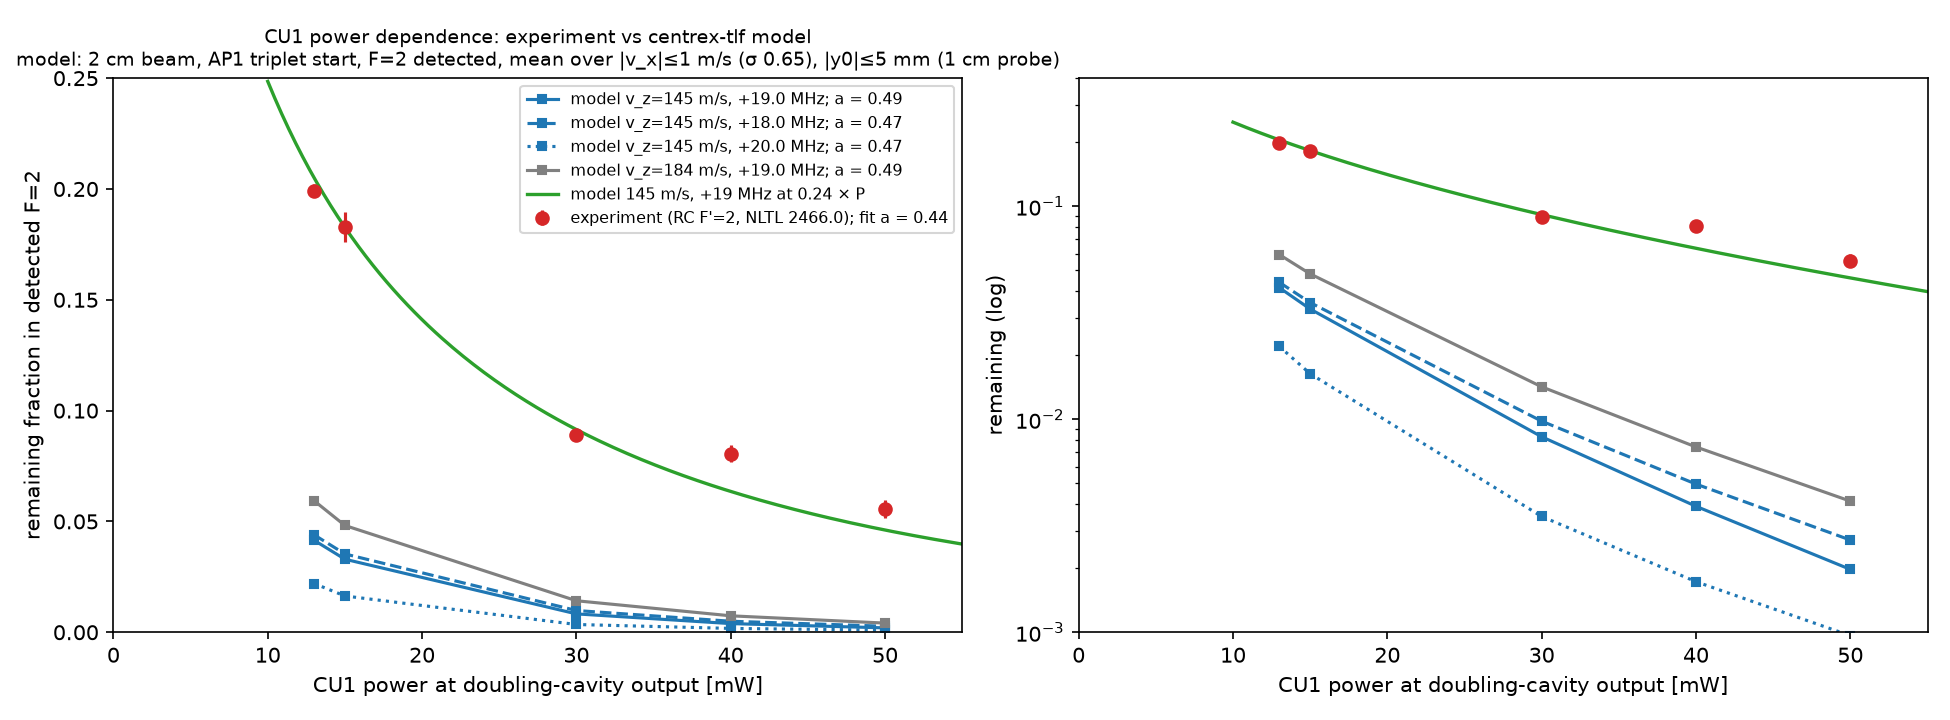
\includegraphics[width=\textwidth]{experiment/exp_B4_old_model_sigma065.png}
  \caption[CU1 test: model with the earlier velocity distribution]{CU1 power dependence: data (10-19,
  RC on $F'=2$, NLTL \SI{2466.0}{MHz}) and the model with the earlier distribution
  ($\sigma_{v_x}=\SI{0.65}{m/s}$, $|v_x|\leq\SI{1}{m/s}$, $|y_0|\leq\SI{5}{mm}$, \SI{2}{cm} beam, AP1 triplet
  start, $F=2$ detected) for several forward velocities and detunings, and the model at 0.24 times the
  power. Left: linear, right: logarithmic scale.}
  \label{fig:exp_oldmodel}
\end{figure}

\begin{figure}[htbp]
  \centering
  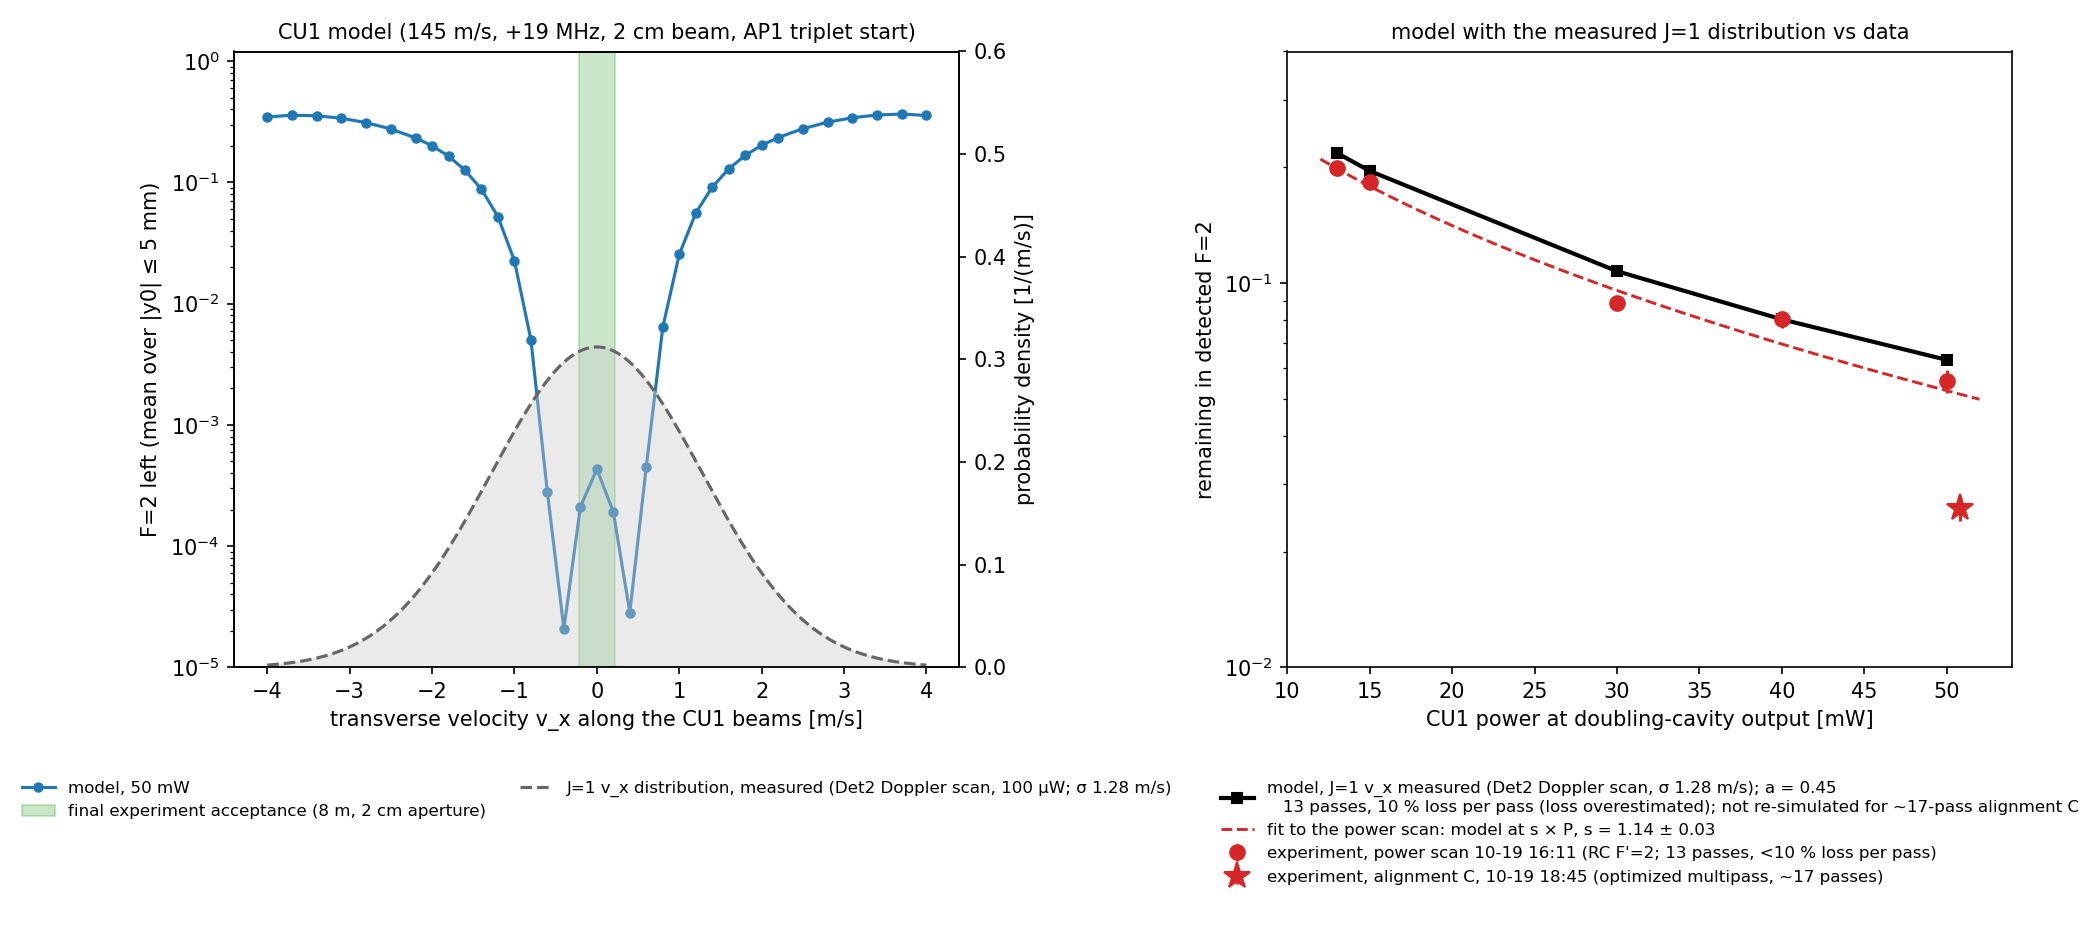
\includegraphics[width=\textwidth]{experiment/exp_10_model_vs_data_measured_vx.png}
  \caption[CU1 test: model with the measured velocity distribution]{CU1 model with the measured $v_x$
  distribution. (a) Remaining $F=2$ population versus $v_x$ at \SI{50}{mW} (\SI{145}{m/s},
  $+\SI{19}{MHz}$, \SI{2}{cm} beam, AP1 triplet start, mean over $|y_0|\leq\SI{5}{mm}$), with the measured
  distribution (grey) and the acceptance of the final experiment (green). (b) The model (13 passes,
  \SI{10}{\percent} loss per pass) against the power scan of 10-19, and its fit with a power scale $s$.}
  \label{fig:exp_model_vx}
\end{figure}

\begin{figure}[htbp]
  \centering
  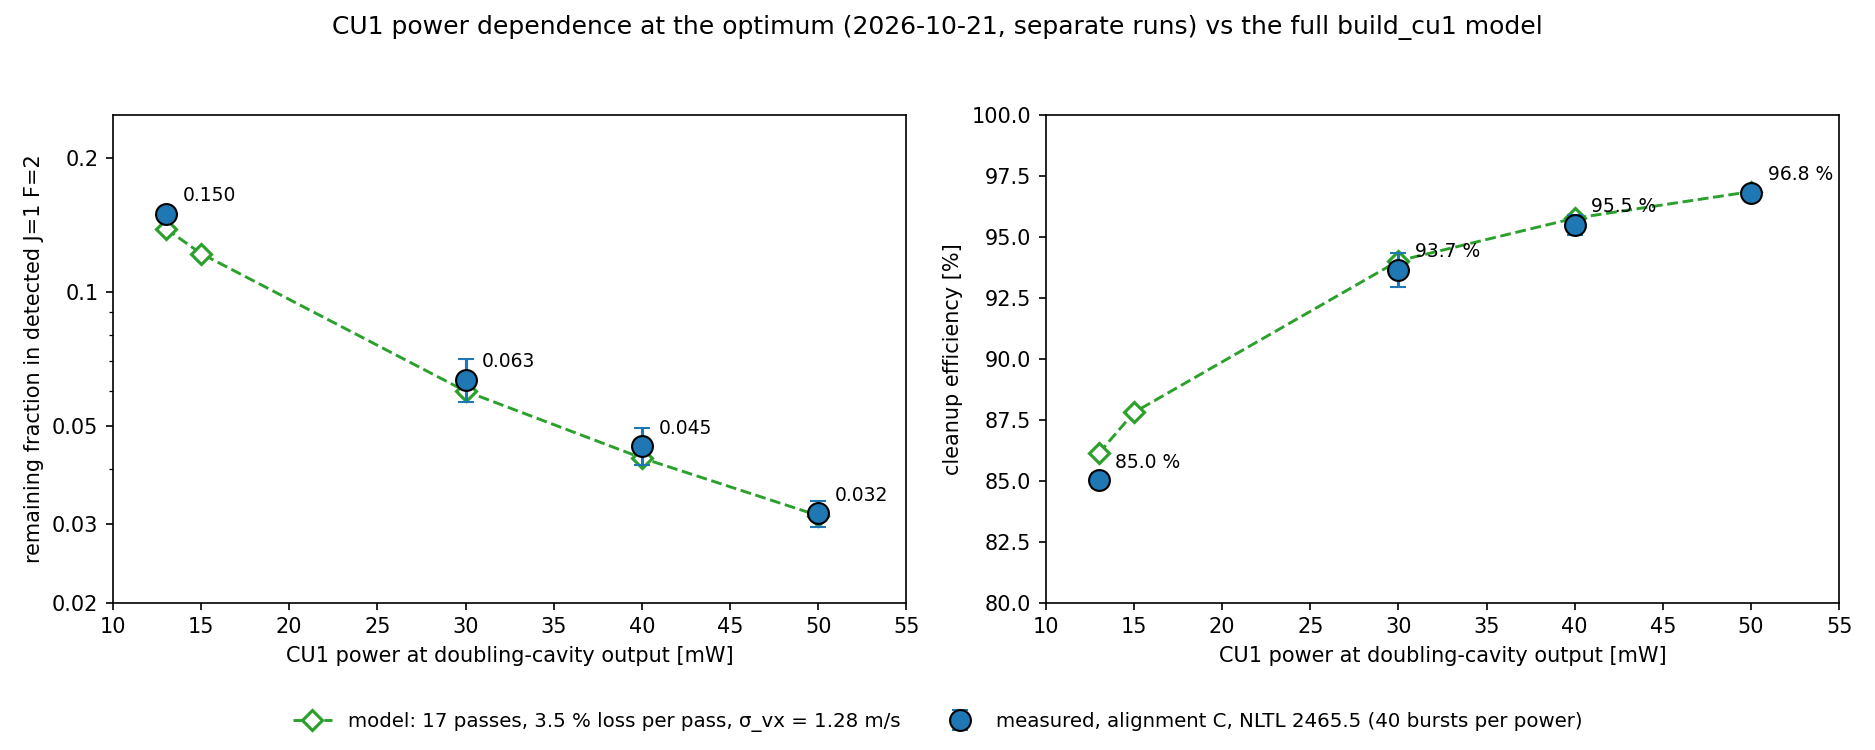
\includegraphics[width=\textwidth]{experiment/exp_12c_power_dependence_vs_model.png}
  \caption[CU1 test: power dependence at the optimum against the full model]{CU1 power dependence at
  the optimum (10-21, alignment C, NLTL \SI{2465.5}{MHz}, 40 bursts per power, R(1) $F'=3$, RC on $F'=2$)
  against the full model (17 passes, \SI{3.5}{\percent} loss per pass, $\sigma_{v_x}=\SI{1.28}{m/s}$).
  Left: remaining fraction, right: efficiency.}
  \label{fig:exp_power_model}
\end{figure}

\begin{figure}[htbp]
  \centering
  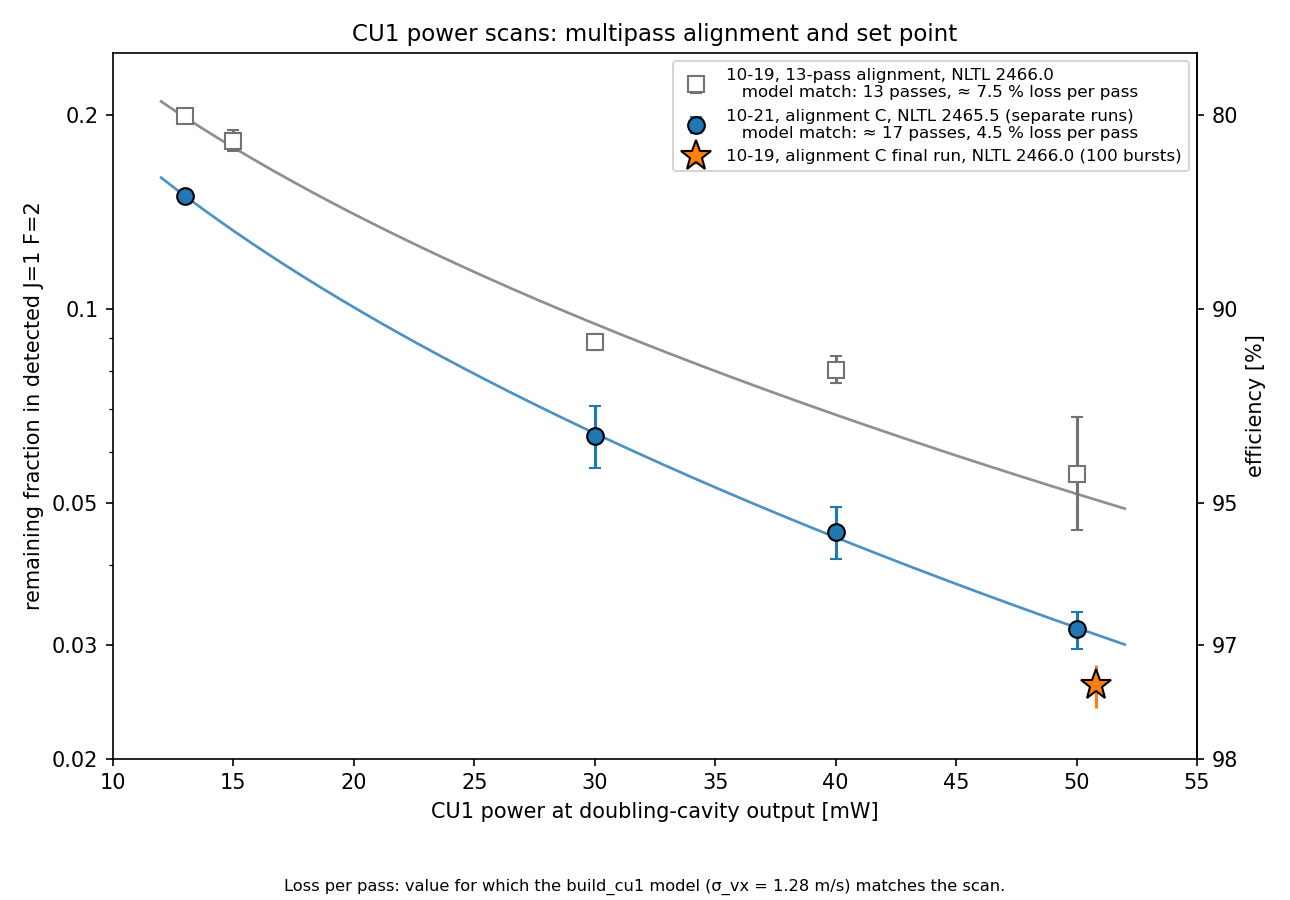
\includegraphics[width=0.75\textwidth]{experiment/exp_12d_power_scans_comparison.png}
  \caption[CU1 test: power scans for two alignments]{CU1 power scans for the 13-pass alignment (10-19,
  NLTL \SI{2466.0}{MHz}) and alignment C (10-21, NLTL \SI{2465.5}{MHz}), and the final run (star). Lines:
  the model ($\sigma_{v_x}=\SI{1.28}{m/s}$) with the loss per pass that matches each scan, as quoted in
  the legend.}
  \label{fig:exp_alignment_model}
\end{figure}

\section{Q(1) detection}
\label{sec:exp_q1}

On 10-21 the detection laser was moved to Q(1) $F_1'=1/2$, $F'=1$ (line position in
Appendix~\ref{app:exp_lines}), with RC on P(2) $F'=1$, the final configuration, and CU1 at NLTL
\SI{2465.5}{MHz}, \SI{50}{mW}, alignment C (240 bursts; Fig.~\ref{fig:exp_q1}). The template fit gives
$r=0.049\ [0.046,0.053]$, i.e.\ \SI{95.1(4)}{\percent}; the window integral gives $0.046\ [0.037,0.054]$,
\SI{95.4(9)}{\percent}. The result does not depend on the absorption cut (0--0.07: $r=0.049$--0.053).
With RC on $F'=2$ the Q(1) ratio was 0.044--0.050, and R(1) gave about 0.03 on the same day. The lower
efficiency is likely due to the incomplete cleanup of other sublevels that Q(1) sees. Because the Q(1)
ratio is not the $J=1$ remaining fraction (Sec.~\ref{sec:exp_detection}), this difference was not
pursued further.

\begin{figure}[htbp]
  \centering
  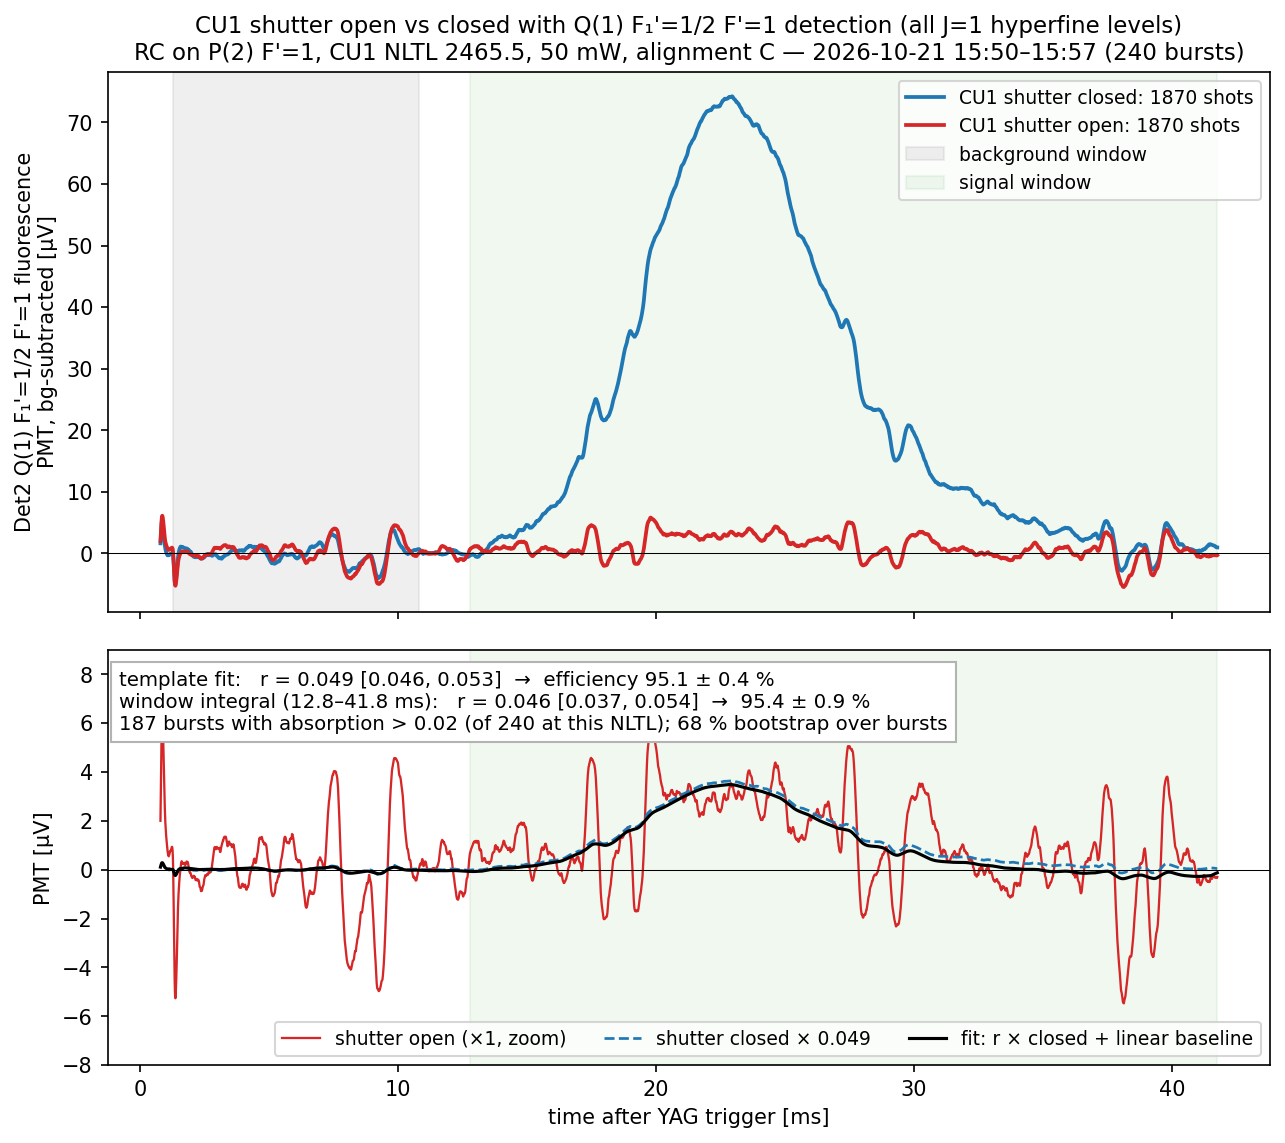
\includegraphics[width=0.72\textwidth]{experiment/exp_14b_Q1_detection_RCF1_240bursts.png}
  \caption[CU1 test: Q(1) detection]{CU1 with Q(1) $F_1'=1/2$, $F'=1$ detection (10-21, RC on P(2)
  $F'=1$, NLTL \SI{2465.5}{MHz}, \SI{50}{mW}, alignment C): mean traces with the shutter closed and open
  (top), and the open-shutter trace with the template fit (bottom), with the results of both
  estimators.}
  \label{fig:exp_q1}
\end{figure}

\section{Open issues}
\label{sec:exp_open}

\begin{enumerate}[itemsep=1pt]
  \item \textbf{Set point.} The measured optimum lies 4--\SI{6}{MHz} (UV) below the predicted
        $+\SI{19}{}$ to $+\SI{20}{MHz}$. Candidates, none evaluated: the model optimum for
        $\sigma_{v_x}=\SI{1.28}{m/s}$ (not recomputed); \SI{150}{V/cm} in the model against \SI{156}{V/cm};
        the \SI{9.1}{MHz} offset of the main pair, taken from the first spectra; drifts of the reference
        cavity (about $\pm\SI{1}{MHz}$) and of the wavemeter (about $+\SI{0.7}{MHz/h}$).
  \item \textbf{Test of the velocity interpretation.} A narrower detection acceptance (slit or smaller
        probe) should lower the remaining fraction; the model of Fig.~\ref{fig:exp_model_vx}a gives the
        expected value for each acceptance.
  \item \textbf{Multipass.} Characterise and reproduce alignment C (pass count, loss per pass);
        reconcile the \SI{3.5}{\percent} and \SI{4.5}{\percent} fits.
  \item \textbf{PMT noise.} Trigger-locked pairs of spikes every \SI{10}{ms} on both PMTs, present since
        10-17 and also with CU1 blocked. They are equal in open and closed shots and cancel in $r$
        (masking them changes 0.0490 to 0.0485); the source is to be found (shutter driver off, shutter
        head unplugged, detection laser blocked).
  \item \textbf{Other.} Record the detection power of the efficiency runs; reduce the CU1 scattered light
        on the PMT; a higher CU1 power; re-run the 17-pass model at \SI{155}{m/s}; check the centre of
        RC P(2) $F'=1$ (Fig.~\ref{fig:exp_rc}).
\end{enumerate}

% =====================================================================
\chapter{CU2 results at \SI{200}{V/cm}}
\label{ch:j2}

\section{Operating field}

CU2 in the experiment now runs at about \SI{200}{V/cm}, and this field is used for all CU2
simulations from here on. Earlier simulations at \SI{250}{V/cm} are collected in
Appendix~\ref{app:legacy}. They are not combined with \SI{200}{V/cm} results, because the
detuning axes refer to field-dependent main resonances (Sec.~\ref{sec:couplings}) and because
$\Dmain$ changes from 219.93 to \SI{211.83}{MHz} (Eq.~\eqref{eq:dmain}). At \SI{200}{V/cm}
one-shot state identification is within its validated range and the build issues no ambiguity
warning.

\section{Configuration}

Baseline of Table~\ref{tab:baseline}, 56-level model (Appendix~\ref{app:code}):
\begin{itemize}
  \item beam~0 on R(2) $F_1'=7/2$, $F'=3$, $P_0=\SI{80}{mW}$; beam~1 on R(2) $F_1'=7/2$,
        $F'=4$, $P_1=\SI{24}{mW}$;
  \item common phase modulation, \SI{17.5}{MHz}, $\beta=1.5$;
  \item X/Z switching at \SI{0.5}{MHz} in antiphase;
  \item common multipass, \SI{10}{\percent} loss per pass, beam height \SI{2.4}{cm};
  \item frequency difference of the beams $\fAOM=200\pm\SI{15}{MHz}$, i.e.\
        $-26.83\leq(\delta_1-\delta_0)/2\pi\leq+\SI{3.17}{MHz}$ (Table~\ref{tab:aom}).
\end{itemize}

\section{Single trajectory at the former set point}

At the detunings that were optimal at \SI{250}{V/cm}, $(\delta_0,\delta_1)/2\pi=(+18.5,
-\SI{6.5}{MHz})$, which at \SI{200}{V/cm} correspond to $\fAOM=\SI{186.83}{MHz}$, the cleanup is
only $\etac=\SI{92.87}{\percent}$, with $\Ngam=1.42$. In the \SI{250}{V/cm} scans the same
detunings ($\fAOM=\SI{194.93}{MHz}$ there) gave \SI{99.99}{\percent}.

\begin{figure}[htbp]
  \centering
  \figplaceholder{CU2_200V_single_trajectory.pdf}
  \caption[CU2 at \SI{200}{V/cm}: populations along the interaction region]{CU2 at
  \SI{200}{V/cm}, single trajectory: populations of the 20 $J=2$ sublevels versus
  distance at $(+18.5,-\SI{6.5}{MHz})$, for comparison with the optima in
  Fig.~\ref{fig:j2_opt_sub}.}
  \label{fig:j2_single}
\end{figure}

\section{Laser-frequency scan at fixed AOM frequency}

In a first scan both detunings were shifted by a common offset, keeping
$(\delta_1-\delta_0)/2\pi=-\SI{25}{MHz}$. This is a scan of the laser frequency at fixed
$\fAOM=\SI{186.83}{MHz}$ (Table~\ref{tab:j2_corr}, Fig.~\ref{fig:j2_corr}). The best point is
an offset of $-\SI{4}{MHz}$, $(\delta_0,\delta_1)/2\pi=(+14.5,-\SI{10.5}{MHz})$, with
$\etac=\SI{99.33}{\percent}$. The cleanup changes by several percent between neighbouring
points, so the \SI{2}{MHz} grid is too coarse. For comparison, the CU1 optimum is about
\SI{1.6}{MHz} wide at the \SI{99.5}{\percent} level.

\begin{table}[htbp]
  \centering
  \caption[CU2 at \SI{200}{V/cm}: laser-frequency scan at fixed AOM frequency]{CU2 at
  \SI{200}{V/cm}: cleanup efficiency versus a common offset of both detunings at fixed
  $\fAOM=\SI{186.83}{MHz}$, i.e.\ $(\delta_1-\delta_0)/2\pi=-\SI{25}{MHz}$ (run
  \code{correlated\_detuning\_shared\_offset\_200V}, rtol $10^{-6}$).}
  \label{tab:j2_corr}
  \small
  \begin{tabular}{rrrc}
    \toprule
    offset (MHz) & $\delta_0/2\pi$ (MHz) & $\delta_1/2\pi$ (MHz) & $\etac$ \\
    \midrule
    $-10$ & 8.5 & $-16.5$ & \SI{96.25}{\percent} \\
    $-8$ & 10.5 & $-14.5$ & \SI{95.88}{\percent} \\
    $-6$ & 12.5 & $-12.5$ & \SI{97.15}{\percent} \\
    $-4$ & 14.5 & $-10.5$ & \textbf{\SI{99.33}{\percent}} \\
    $-2$ & 16.5 & $-8.5$ & \SI{97.96}{\percent} \\
    $0$ & 18.5 & $-6.5$ & \SI{92.94}{\percent} \\
    $+2$ & 20.5 & $-4.5$ & \SI{91.06}{\percent} \\
    $+4$ & 22.5 & $-2.5$ & \SI{96.46}{\percent} \\
    $+6$ & 24.5 & $-0.5$ & \SI{97.24}{\percent} \\
    $+8$ & 26.5 & $1.5$ & \SI{96.14}{\percent} \\
    \bottomrule
  \end{tabular}
\end{table}

\begin{figure}[htbp]
  \centering
  \figplaceholder{CU2_200V_laser_frequency_scan.pdf}
  \caption[CU2: laser-frequency scan at 200 and \SI{250}{V/cm}]{CU2 cleanup versus the common
  detuning offset at \SI{200}{V/cm} ($\fAOM=\SI{186.83}{MHz}$, Table~\ref{tab:j2_corr}) and,
  for reference, at \SI{250}{V/cm} ($\fAOM=\SI{194.93}{MHz}$, Appendix~\ref{app:legacy}).
  Lower axis: $\delta_0$; upper axis: $\delta_1$.}
  \label{fig:j2_corr}
\end{figure}

\section{Why the \SI{250}{V/cm} set point does not carry over}

The field change moves the two manifolds relative to each other. $\Dmain$ decreases by
\SI{8.1}{MHz}, and the component positions within each manifold (Table~\ref{tab:spread}) move
as well. With the AOM frequency of the former optimum, \SI{194.93}{MHz}, the detuning
difference at \SI{200}{V/cm} would be $-\SI{16.9}{MHz}$ instead of $-\SI{25}{MHz}$. With the
former detuning difference, the AOM must be set to \SI{186.83}{MHz}. Neither choice
reproduces the former alignment of both beams with their manifolds, and a scan of the laser
frequency alone, at one AOM frequency, cannot find the new optimum. Laser frequency and AOM
frequency must be optimised together.

\section{Two-dimensional optimisation in laser and AOM frequency}
\label{sec:j2_2d}

The optimisation uses the experimental coordinates $(\delta_0,\fAOM)$, with $\delta_1$ from
Eq.~\eqref{eq:aom} and $\Dmain=\SI{211.829}{MHz}$ computed from the model. It was run in three
stages with \code{scripts/cu2\_laser\_aom\_scan.py} (Appendix~\ref{app:code}), using the scan
tolerances of Table~\ref{tab:solver}.
\begin{enumerate}
  \item \textbf{Coarse grid}, \SI{2}{MHz} steps: $\delta_0/2\pi=+5\ldots+\SI{23}{MHz}$ (about
        one EOM period around the earlier best point) $\times$ $\fAOM=185\ldots\SI{215}{MHz}$
        (the full AOM range), 160 points.
  \item \textbf{Fine grids}, \SI{0.5}{MHz} steps over $\pm\SI{2}{MHz}$ around the three best
        separated local maxima of the coarse grid, 219 further points.
  \item \textbf{Confirmation} of the three best points with rtol $10^{-7}$, atol $10^{-9}$.
\end{enumerate}

\subsection{Coarse grid}

The cleanup varies between \SI{86.1}{\percent} and \SI{99.79}{\percent} over the grid
(Fig.~\ref{fig:j2_map}). Only 15 of the 160 points exceed \SI{99}{\percent}, and 6 exceed
\SI{99.5}{\percent}. The best points lie in two groups at $\delta_0/2\pi\approx\num{11}$ to
\SI{13}{MHz}, one with $\delta_1/2\pi\approx+\SI{8}{MHz}$ ($\fAOM\approx\SI{208}{MHz}$) and one
with $\delta_1/2\pi\approx-\SI{10}{MHz}$ ($\fAOM\approx\SI{190}{MHz}$). The two groups are
separated by about one EOM period in $\delta_1$: the $F'=4$ beam reaches the same components with
its carrier or with an adjacent sideband. A third, weaker maximum lies at the edge of the
$\delta_0$ range, near $\delta_0/2\pi=\SI{23}{MHz}$, $\fAOM=\SI{197}{MHz}$. At
$\fAOM=\SI{187}{MHz}$, next to the line of the earlier laser-frequency scan, the best grid value
is \SI{99.48}{\percent} at $\delta_0/2\pi=\SI{15}{MHz}$, consistent with the \SI{99.33}{\percent}
found there at $(14.5,\SI{186.83}{MHz})$. The earlier optimum is therefore only a side maximum.

\subsection{Fine grids and optimum}

Table~\ref{tab:j2_fine} summarises the three fine grids. The overall optimum lies in region~2:
\begin{equation}
  \frac{\delta_0}{2\pi}=+\SI{11.5}{MHz},\qquad \fAOM=\SI{191.0}{MHz}\quad
  \Bigl(\frac{\delta_1}{2\pi}=-\SI{9.33}{MHz}\Bigr),\qquad \etac=\SI{99.85}{\percent}.
\end{equation}
Region~1 gives almost the same cleanup, \SI{99.80}{\percent}, at
$(+\SI{11.5}{MHz},\SI{208.5}{MHz})$, $\delta_1/2\pi=+\SI{8.17}{MHz}$. Both points lie well
inside the AOM range. Compared with the first laser-frequency scan at fixed AOM frequency, the
remaining population falls from \SI{0.67}{\percent} to \SI{0.15}{\percent}.

\begin{table}[htbp]
  \centering
  \caption[CU2 at \SI{200}{V/cm}: fine grids]{CU2 at \SI{200}{V/cm}: best point of each
  \SI{0.5}{MHz} fine grid (runs \code{laser\_AOM\_2D\_200V\_fine\_0p5MHz\_region1--3}).}
  \label{tab:j2_fine}
  \small
  \begin{tabular}{lccccc}
    \toprule
    region & coarse maximum & best $\delta_0/2\pi$ & best $\fAOM$ & $\delta_1/2\pi$ & $\etac$ \\
    \midrule
    1 & $(11, 209)$\,MHz, \SI{99.79}{\percent} & \SI{11.5}{MHz} & \SI{208.5}{MHz} & $+\SI{8.17}{MHz}$ & \SI{99.80}{\percent} \\
    2 & $(11, 191)$\,MHz, \SI{99.77}{\percent} & \SI{11.5}{MHz} & \SI{191.0}{MHz} & $-\SI{9.33}{MHz}$ & \textbf{\SI{99.85}{\percent}} \\
    3 & $(23, 197)$\,MHz, \SI{99.55}{\percent} & \SI{23.5}{MHz} & \SI{196.5}{MHz} & $+\SI{8.17}{MHz}$ & \SI{99.56}{\percent} \\
    \bottomrule
  \end{tabular}
\end{table}

\subsection{Confirmation with tighter tolerances}

The three best points, all in region~2, were recomputed with rtol $10^{-7}$
(Table~\ref{tab:j2_confirm}). The cleanup changes by \num{3e-5} at most, so the scan
tolerance is adequate at the optimum.

\begin{table}[htbp]
  \centering
  \caption[CU2 at \SI{200}{V/cm}: confirmation of the best points]{CU2 at \SI{200}{V/cm}:
  best points recomputed with rtol $10^{-7}$, atol $10^{-9}$ (run
  \code{laser\_AOM\_2D\_200V\_confirm\_rtol1e-7}).}
  \label{tab:j2_confirm}
  \small
  \begin{tabular}{cccc}
    \toprule
    $\delta_0/2\pi$ & $\fAOM$ & $\etac$, rtol $10^{-6}$ & $\etac$, rtol $10^{-7}$ \\
    \midrule
    \SI{11.5}{MHz} & \SI{191.0}{MHz} & \SI{99.8535}{\percent} & \SI{99.8508}{\percent} \\
    \SI{11.0}{MHz} & \SI{191.5}{MHz} & \SI{99.8352}{\percent} & \SI{99.8319}{\percent} \\
    \SI{12.0}{MHz} & \SI{190.5}{MHz} & \SI{99.8301}{\percent} & \SI{99.8275}{\percent} \\
    \bottomrule
  \end{tabular}
\end{table}

\subsection{Width of the optimum}

Table~\ref{tab:j2_window} gives the ranges over which the cleanup stays above a given level,
along the laser frequency at fixed AOM frequency and along the AOM frequency at fixed laser
frequency. A shift along the laser frequency is also what a common shift of both lines
produces, for example from a change of the electric field. Both optima are 0.5--\SI{1.5}{MHz}
wide at the \SI{99.7}{\percent} level and 2--\SI{3}{MHz} wide at \SI{99}{\percent}.
Region~2 has the higher peak, and region~1 is somewhat wider, in particular along the AOM
frequency. The design-study estimate of a \SI{2}{MHz} line shift from the field variation
across the cleanup region (Fig.~\ref{fig:efield}) is comparable to the \SI{99}{\percent} width,
so the field uniformity at \SI{200}{V/cm} should be checked.

The fine grids also show that both optima are elongated along lines of constant $\delta_1$,
$\delta_0+2\pi\fAOM=\text{const}$ (Fig.~\ref{fig:j2_fine}). Along such a line, i.e.\ with the
$F'=4$ detuning held fixed, the cleanup in region~2 stays above \SI{99.6}{\percent} for
$\delta_0/2\pi$ from 10.0 to \SI{13.0}{MHz}. Moving across it, a change of $\delta_0$ by
\SI{0.5}{MHz} combined with a change of $\delta_1$ by \SI{1}{MHz} already lowers the cleanup to
\SI{99.4}{\percent}. The efficiency is therefore set mainly by the detuning of the $F'=4$ beam:
$\delta_1$ must be held to about $\pm\SI{0.5}{MHz}$, while $\delta_0$ tolerates about
$\pm\SI{1.5}{MHz}$ if $\delta_1$ is kept fixed. Since a drift of the laser frequency shifts both
detunings together, the laser frequency is limited by the tighter $\delta_1$ tolerance.

\begin{table}[htbp]
  \centering
  \caption[CU2 at \SI{200}{V/cm}: width of the optima]{CU2 at \SI{200}{V/cm}: ranges (on the
  \SI{0.5}{MHz} grid) within which the cleanup exceeds the given level, through the best point
  of regions~1 and~2.}
  \label{tab:j2_window}
  \small
  \begin{tabular}{llccc}
    \toprule
    region & direction & $>\SI{99.7}{\percent}$ & $>\SI{99.5}{\percent}$ & $>\SI{99}{\percent}$ \\
    \midrule
    2 & $\delta_0/2\pi$ at $\fAOM=\SI{191.0}{MHz}$ & 11.0--\SI{12.0}{MHz} & 11.0--\SI{12.0}{MHz} & 10.5--\SI{12.5}{MHz} \\
    2 & $\fAOM$ at $\delta_0/2\pi=\SI{11.5}{MHz}$ & 190.5--\SI{191.5}{MHz} & 190.0--\SI{191.5}{MHz} & 189.5--\SI{192.0}{MHz} \\
    1 & $\delta_0/2\pi$ at $\fAOM=\SI{208.5}{MHz}$ & 11.5--\SI{12.0}{MHz} & 11.0--\SI{12.5}{MHz} & 10.5--\SI{13.0}{MHz} \\
    1 & $\fAOM$ at $\delta_0/2\pi=\SI{11.5}{MHz}$ & 208.0--\SI{209.5}{MHz} & 208.0--\SI{210.0}{MHz} & 207.5--\SI{210.5}{MHz} \\
    \bottomrule
  \end{tabular}
\end{table}

\begin{figure}[htbp]
  \centering
  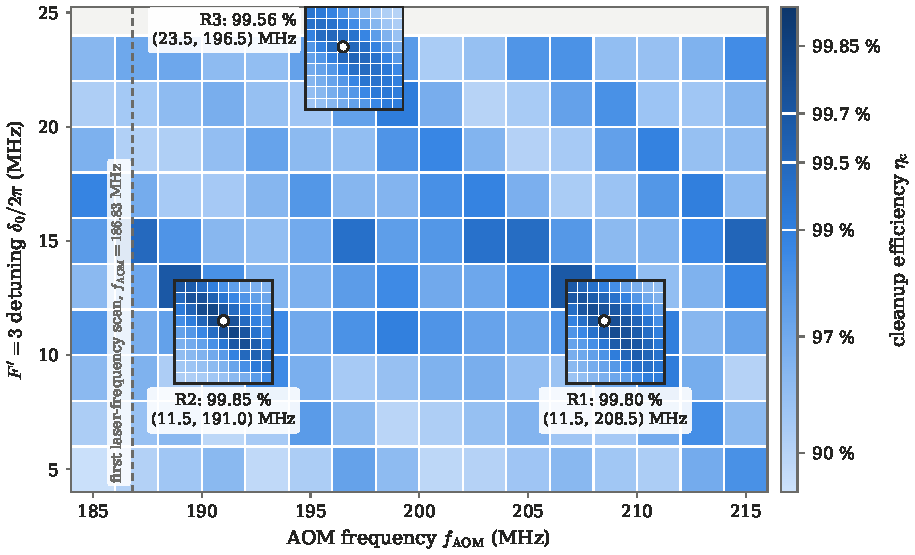
\includegraphics[width=\textwidth]{CU2_200V_laser_AOM_map.pdf}
  \caption[CU2 at \SI{200}{V/cm}: cleanup versus laser and AOM frequency]{CU2 cleanup
  efficiency at \SI{200}{V/cm} versus the AOM frequency $\fAOM$ (full range
  185--\SI{215}{MHz}) and the $F'=3$ detuning $\delta_0$, i.e.\ the laser frequency. Colour:
  remaining $J=2$ population on a logarithmic scale, labelled in cleanup efficiency; darker is
  better; white lines on the colour bar mark 99, 99.5 and \SI{99.7}{\percent}. Large cells: coarse
  \SI{2}{MHz} grid (run \code{laser\_AOM\_2D\_200V\_coarse\_2MHz}); outlined boxes: \SI{0.5}{MHz}
  fine grids R1--R3, with their best points (circles). Dashed: the line
  $\fAOM=\SI{186.83}{MHz}$ of the first laser-frequency scan. The grey band above
  $\delta_0/2\pi=\SI{24}{MHz}$ was not computed outside R3.}
  \label{fig:j2_map}
\end{figure}

\begin{figure}[htbp]
  \centering
  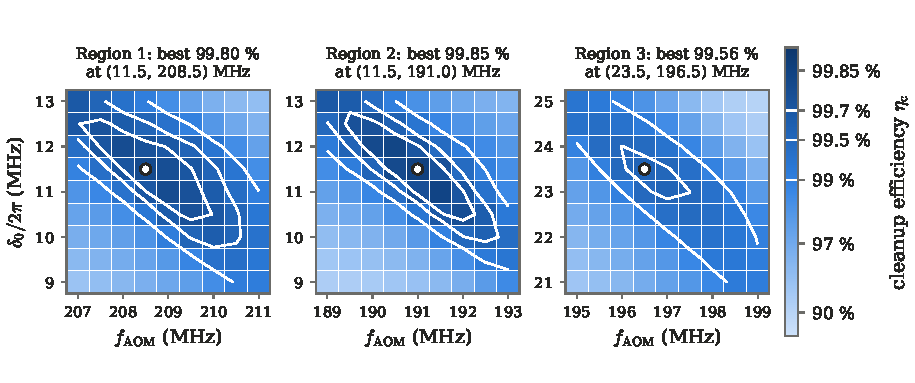
\includegraphics[width=\textwidth]{CU2_200V_fine_regions.pdf}
  \caption[CU2 at \SI{200}{V/cm}: fine grids around the optima]{CU2 at \SI{200}{V/cm}:
  \SI{0.5}{MHz} fine grids R1--R3 (runs \code{laser\_AOM\_2D\_200V\_fine\_0p5MHz\_region1--3}),
  same colour scale as Fig.~\ref{fig:j2_map}. White contours: 99, 99.5 and
  \SI{99.7}{\percent}; circles: best points. The high-efficiency areas run along lines of
  constant $\delta_1$ (slope $-1$).}
  \label{fig:j2_fine}
\end{figure}

\subsection{Trajectories at the two optima}
\label{sec:j2_traj}

Single trajectories at the best points of R1 and R2 were computed with rtol $10^{-7}$, saving
the populations every \SI{0.1}{\micro\second}. The photon number was taken from the solver's
running integral (\code{output="photon\_integral"}) rather than from the sampled excited
population. The script is \code{scripts/cu2\_optimum\_trajectories.py}.
Figures~\ref{fig:j2_opt_pop} and~\ref{fig:j2_opt_sub} show the result, and
Table~\ref{tab:j2_opt} lists the final populations.

\begin{itemize}
  \item \textbf{Pass by pass.} The first pass removes about \SI{75}{\percent} of the $J=2$
        population. Each later pass multiplies what is left by 0.5 to 0.8, following the
        alternating powers of the multipass passes: strong passes remove more. The population
        still falls at the last pass, so more passes or more power would improve the cleanup
        further.
  \item \textbf{Destination.} The removed molecules end almost entirely in $J=3$ (53--54\,\%) and
        $J=4$ (44--45\,\%), with \SI{1.7}{\percent} in $J=5$ and $3\times10^{-5}$ in $J=1$. The
        excited-state population peaks at \SI{1.4}{\percent} in the first pass. Each molecule
        scatters 1.5 photons on average.
  \item \textbf{Bottleneck.} The remaining population is dominated by the stretched sublevels
        $|F_1=\tfrac52,F=3,m_F=\pm3\rangle$: \SI{74}{\percent} of it in R1 and \SI{56}{\percent}
        in R2. Next come the $F_1=\tfrac32$, $F=2$ sublevels, \SI{18}{\percent} in R1 and
        \SI{35}{\percent} in R2. R2 cleans the stretched sublevels better, which is why its
        total is lower.
  \item \textbf{Tolerance check.} With rtol $10^{-7}$ the R1 optimum gives \SI{99.823}{\percent},
        against \SI{99.803}{\percent} in the scan; the R2 value, \SI{99.851}{\percent}, agrees with
        Table~\ref{tab:j2_confirm}.
\end{itemize}

\begin{table}[htbp]
  \centering
  \caption[CU2 at \SI{200}{V/cm}: final populations at the two optima]{CU2 at \SI{200}{V/cm}:
  final populations at the two optima (rtol $10^{-7}$), and the photon number per molecule from
  the running integral.}
  \label{tab:j2_opt}
  \small
  \begin{tabular}{lcc}
    \toprule
    & R1 & R2 \\
    \midrule
    $(\delta_0/2\pi,\ \fAOM,\ \delta_1/2\pi)$ (MHz) & $(11.5,\ 208.5,\ +8.17)$ & $(11.5,\ 191.0,\ -9.33)$ \\
    cleanup efficiency $\etac$ & \SI{99.823}{\percent} & \textbf{\SI{99.851}{\percent}} \\
    remaining in $J=2$ & $1.77\times10^{-3}$ & $1.49\times10^{-3}$ \\
    \quad of which $F_1=\tfrac52$, $F=3$, $m_F=\pm3$ & \SI{74}{\percent} & \SI{56}{\percent} \\
    \quad of which $F_1=\tfrac32$, $F=2$ & \SI{18}{\percent} & \SI{35}{\percent} \\
    $J=3$ & 0.541 & 0.529 \\
    $J=4$ & 0.439 & 0.452 \\
    $J=5$ & 0.0177 & 0.0173 \\
    $J=1$ & $3.2\times10^{-5}$ & $3.3\times10^{-5}$ \\
    photons per molecule $\Ngam$ & 1.50 & 1.51 \\
    \bottomrule
  \end{tabular}
\end{table}

\begin{figure}[htbp]
  \centering
  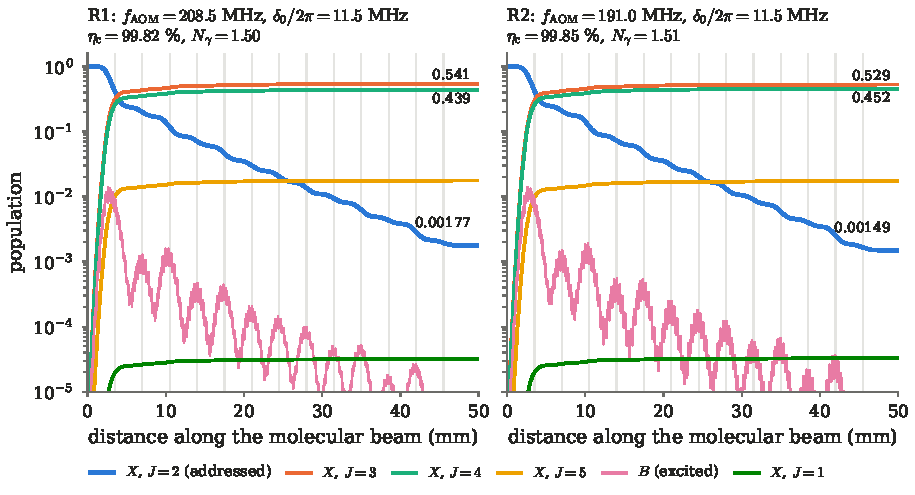
\includegraphics[width=\textwidth]{CU2_200V_optimum_populations.pdf}
  \caption[CU2 at \SI{200}{V/cm}: rotational-level populations at the two optima]{CU2 at
  \SI{200}{V/cm}: populations of the rotational levels along the interaction region at the
  optima of R1 ($\delta_1/2\pi=+\SI{8.17}{MHz}$) and R2 ($\delta_1/2\pi=-\SI{9.33}{MHz}$),
  logarithmic scale. Grey vertical lines: centres of the 13 passes. The excited-state population
  oscillates with the \SI{0.5}{MHz} polarization switching and the \SI{17.5}{MHz} phase
  modulation; it is sampled every \SI{0.1}{\micro\second}.}
  \label{fig:j2_opt_pop}
\end{figure}

\begin{figure}[htbp]
  \centering
  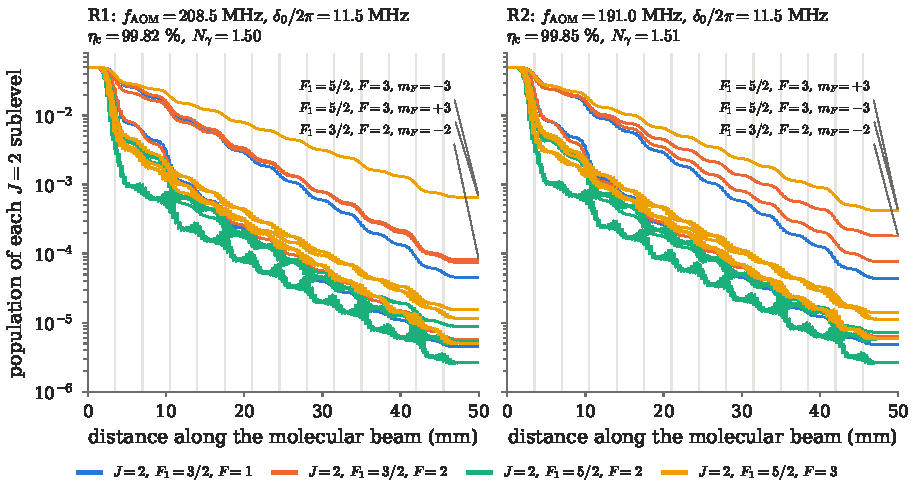
\includegraphics[width=\textwidth]{CU2_200V_optimum_J2_sublevels.pdf}
  \caption[CU2 at \SI{200}{V/cm}: $J=2$ sublevel populations at the two optima]{CU2 at
  \SI{200}{V/cm}: populations of the 20 $J=2$ sublevels at the optima of R1 and R2, coloured by
  hyperfine level $(F_1,F)$; the three sublevels with the most population left are labelled.
  In R1 the two stretched sublevels $m_F=\pm3$ end at the same value.}
  \label{fig:j2_opt_sub}
\end{figure}

\subsection{Why both AOM frequencies work}
\label{sec:j2_two_aom}

Figure~\ref{fig:j2_scheme} shows the excited sublevels addressed by the two beams at
\SI{200}{V/cm}, together with the carrier and sidebands of each beam at the two optima. Its
frequency axis is measured from the $F'=3$ main resonance, so the $F'=4$ sublevels and the
beam-1 lines appear \SI{211.83}{MHz} higher than on the $\delta_1$ axis used in the text and in
Table~\ref{tab:j2_comb}. Each sublevel is placed at the coupling-weighted mean of its
resonances from the 20 $J=2$ sublevels; the ground-state hyperfine structure spreads them by at
most \SI{1.5}{MHz}. Which sublevels the light actually drives is estimated with a weak-field
excitation rate. For sublevel $e$ this is
\begin{equation}
  R_e=\sum_{g\in J=2}\ \sum_{p}|M^{(p)}_{eg}|^2\sum_n J_n(\beta)^2\,
  \frac{1}{1+\bigl[2(\nu_{eg}-\nu_n)/(\Gamma/2\pi)\bigr]^2},
  \label{eq:rate}
\end{equation}
with $\nu_{eg}$ the resonance of the pair and $\nu_n$ the comb lines; saturation, the
polarization switching and coherent effects are not included. The explanation follows from three
observations.

\begin{enumerate}
  \item \textbf{The two settings differ by exactly one EOM period.} The AOM frequencies differ
        by $208.5-191.0=\SI{17.5}{MHz}$, the EOM frequency, while beam~0 is unchanged. The comb
        of beam~1, at $\delta_1/2\pi+n\times\SI{17.5}{MHz}$, therefore occupies the same
        frequencies in R1 and R2. Only the order $n$ of each line shifts by one: the line that is
        the carrier in R1 is the first-order sideband in R2, and so on (upper half of
        Fig.~\ref{fig:j2_scheme}).
  \item \textbf{Carrier and first-order sidebands carry almost the same power.} At $\beta=1.5$
        the carrier carries $J_0^2=\SI{26}{\percent}$ of the power and each first-order
        sideband $J_1^2=\SI{31}{\percent}$. The two lines that matter most sit on the strongest
        $F'=4$ components in both settings: the line at $+\SI{8.17}{MHz}$ on $m_F'=0$
        ($+\SI{8.65}{MHz}$, the most strongly coupled $F'=4$ sublevel), and the line at
        $-\SI{9.33}{MHz}$ on $m_F'=\pm2$ ($-\SI{10.32}{MHz}$). These two components are
        \SI{19.0}{MHz} apart, close to the comb spacing, so two adjacent lines can sit on both at
        once. Whether the carrier or a first-order sideband does the work changes the power on
        each by only about \SI{16}{\percent} (Table~\ref{tab:j2_comb}).
  \item \textbf{The outer lines decide which setting is slightly better.} By
        Eq.~\eqref{eq:rate}, beam~1 drives mainly $m_F'=0$ in both settings, and $m_F'=\pm2$ at
        \SI{35}{\percent} of that rate in R1 and \SI{25}{\percent} in R2. All other $F'=4$
        sublevels stay below \SI{4}{\percent}. The bottleneck of Table~\ref{tab:j2_opt}, the
        stretched ground sublevels $|F_1=\tfrac52,F=3,m_F=\pm3\rangle$, is hardly pumped by
        beam~0: its rate through $F'=3$ is 40 to 50 times lower than through $F'=4$. In $F'=4$ it
        couples mainly to $m_F'=\pm4$ ($-\SI{31.41}{MHz}$) and $m_F'=\pm3$
        ($-\SI{20.44}{MHz}$), which lie far from the two main lines. R2 has a first-order sideband
        (\SI{31}{\percent}) at $-\SI{26.83}{MHz}$, \SI{4.6}{MHz} from the strongly coupled
        $m_F'=\pm4$; R1 has only a second-order sideband there (\SI{5}{\percent}). The
        stretched sublevels are therefore pumped \SI{15}{\percent} faster in R2. R1 in turn has
        \SI{31}{\percent} instead of \SI{26}{\percent} on $m_F'=\pm2$, and pumps the
        $F_1=\tfrac32$, $F=2$ sublevels \SI{11}{\percent} faster. Both trends agree with the
        composition of the remaining population: the stretched sublevels are \SI{56}{\percent} of
        it in R2 against \SI{74}{\percent} in R1, and $F_1=\tfrac32$, $F=2$ is \SI{35}{\percent}
        against \SI{18}{\percent}. Since the stretched sublevels are the main bottleneck, R2 ends
        with less population left, \SI{99.85}{\percent} against \SI{99.82}{\percent}.
\end{enumerate}

Because the comb repeats every \SI{17.5}{MHz}, the optimum repeats every \SI{17.5}{MHz} in
$\fAOM$. Within the AOM range only these two copies exist: the next ones, at 173.5 and
\SI{226}{MHz}, lie outside 185--\SI{215}{MHz}. Beam~0 is the same in both settings. Its
first-order sideband sits on the $F'=3$, $m_F'=\pm1$ components ($+\SI{28.41}{MHz}$), and its
carrier lies \SI{3}{MHz} below the $m_F'=\pm2$ components.

\begin{table}[htbp]
  \centering
  \caption[CU2: beam-1 comb lines and $F'=4$ sublevels at the two optima]{CU2 at
  \SI{200}{V/cm}: comb lines of beam~1 near the $F'=4$ sublevels, with their order $n$ and power
  fraction $J_n(1.5)^2$ in R1 and R2. Positions on the $\delta_1$ axis.}
  \label{tab:j2_comb}
  \small
  \begin{tabular}{rlcc}
    \toprule
    line (MHz) & nearest $F'=4$ sublevel(s) & R1: $n$, power & R2: $n$, power \\
    \midrule
    $+8.17$ & $m_F'=0$, $P'=-$ at $+8.65$ (strongest) & $0$, \SI{26}{\percent} & $+1$, \SI{31}{\percent} \\
    $-9.33$ & $m_F'=\pm2$, $P'=-$ at $-10.32$ & $-1$, \SI{31}{\percent} & $0$, \SI{26}{\percent} \\
    $+25.67$ & $m_F'=\pm1$, $P'=+$ at $+22.50$ & $+1$, \SI{31}{\percent} & $+2$, \SI{5}{\percent} \\
    $-26.83$ & $m_F'=\pm3$ at $-20.83$, $\pm4$ at $-31.41$, $P'=-$ & $-2$, \SI{5}{\percent} & $-1$, \SI{31}{\percent} \\
    $+43.17$ & $m_F'=\pm3$, $P'=+$ at $+44.43$ & $+2$, \SI{5}{\percent} & $+3$, \SI{0.4}{\percent} \\
    \bottomrule
  \end{tabular}
\end{table}

\begin{figure}[htbp]
  \centering
  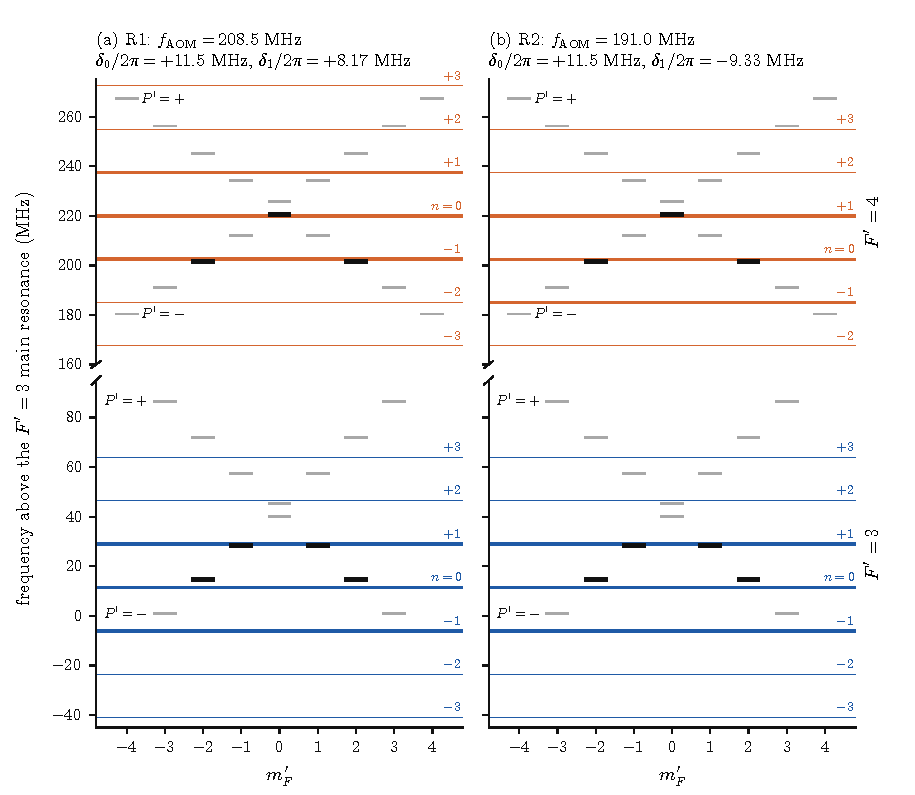
\includegraphics[width=\textwidth]{CU2_200V_level_diagram_R1_R2.pdf}
  \caption[CU2 at \SI{200}{V/cm}: level diagram with the laser combs of R1 and R2]{CU2 at
  \SI{200}{V/cm}: excited sublevels of $B$, $J'=3$, $F_1'=7/2$ addressed from $X$, $J=2$, and
  the laser combs at the optima of (a) R1 and (b) R2. The frequency axis is broken between
  $F'=3$ (bottom) and $F'=4$ (top) and gives the transition frequency above the $F'=3$ main
  resonance; the $F'=4$ main resonance lies at \SI{211.83}{MHz}. Each dash is one excited
  sublevel at the coupling-weighted mean of its resonances from the 20 $J=2$ sublevels (which
  span at most \SI{1.5}{MHz}). The two $\Lambda$-doublet components with the same $m_F'$ are
  aligned vertically and form the $P'=-$ and $P'=+$ branches. Sublevels driven by the light,
  with an excitation rate, Eq.~\eqref{eq:rate}, of at least \SI{5}{\percent} of the most strongly
  driven sublevel of the same beam, are shown in bold. Coloured lines: carrier ($n=0$) and
  phase-modulation sidebands $n$ of beam~0 (blue, $F'=3$) and beam~1 (orange, $F'=4$), with line
  width proportional to the power fraction $J_n(1.5)^2$ (0.26, 0.31, 0.05 and 0.004 for
  $|n|=0$--3). Beam~0 is the same in (a) and (b). The beam-1 lines lie at the same frequencies in
  both columns, and only their orders differ by one. Script: \code{scripts/cu2\_level\_scheme.py}.}
  \label{fig:j2_scheme}
\end{figure}

\section{Transverse velocity and position at the present beam height}
\label{sec:j2_doppler}

\paragraph{Setup.} The two optima were evaluated over the transverse velocity and position
under the present conditions of Sec.~\ref{sec:j1_present}: beam height \SI{3}{cm}
($\sigy=\SI{7.5}{mm}$) at the same 80 + \SI{24}{mW}, i.e.\ 0.8 times the peak intensity of the
\SI{2.4}{cm} beam used for the optimisation (\code{build(sigma\_y\_m=7.5e-3)}). The two beams run
through the same multipass in the same direction, so the Doppler shift, Eq.~\eqref{eq:doppler},
is common to both: in the $(\delta_0,\fAOM)$ plane it moves the operating point along the laser
frequency at fixed AOM frequency, in alternate directions in alternate passes. A coarse grid
was computed, $v_x$ from $-1$ to $+\SI{1}{m/s}$ in steps of \SI{0.2}{m/s} and $y_0$ from 0 to
\SI{15}{mm} in steps of \SI{3}{mm} (66 trajectories, about \SI{50}{min} per run), for R1 and R2
and for two initial states, all 20 $J=2$ sublevels and the four SPB source levels ($J=2$,
$m_J=0$, lens weights 2/3 for the singlet and 1/9 for each triplet level) (script
\code{scripts/cu2\_doppler\_scan.py}, runs \code{doppler\_cu2\_\{R1,R2\}\_\{uniform,spb\}\_3cm\_coarse}).
The means use the beam-simulation distribution at CU2 (lens + \SI{1.0}{m}): $\sigma_{v_x}=\SI{0.65}{m/s}$
and $\sigma_y=\SI{10.35}{mm}$, within the detection acceptance $|v_x|\leq\SI{1}{m/s}$,
$|y_0|\leq\SI{8.5}{mm}$.

\begin{table}[htbp]
  \centering
  \caption[CU2: cleanup over the transverse distribution]{CU2 at \SI{200}{V/cm} with the
  \SI{3}{cm} beam: cleanup on the axis, averaged over $v_x$ at $y_0=0$, and mean in the detection
  acceptance; for comparison, the mean with the $y_0$ range extended to \SI{15}{mm} (coarse
  grid, beam-simulation weights). The recommended setting is in bold.}
  \label{tab:j2_doppler}
  \small
  \setlength{\tabcolsep}{4pt}
  \begin{tabular}{llcccc}
    \toprule
    $\fAOM$ & start & on axis & $v_x$-av., $y_0=0$ & \textbf{in acceptance} & $|y_0|\leq\SI{15}{mm}$ \\
    \midrule
    R2, \SI{191.0}{MHz} & all 20 sublevels & \SI{99.59}{\percent} & \SI{97.72}{\percent} & \SI{96.10}{\percent} & \SI{91.84}{\percent} \\
    \textbf{R1}, \SI{208.5}{MHz} & all 20 sublevels & \SI{99.52}{\percent} & \SI{98.16}{\percent} & \textbf{\SI{96.66}{\percent}} & \SI{92.51}{\percent} \\
    R2, \SI{191.0}{MHz} & SPB source levels & \SI{99.975}{\percent} & \SI{99.67}{\percent} & \SI{99.35}{\percent} & \SI{98.42}{\percent} \\
    \textbf{R1}, \SI{208.5}{MHz} & SPB source levels & \SI{99.974}{\percent} & \SI{99.81}{\percent} & \textbf{\SI{99.57}{\percent}} & \SI{98.79}{\percent} \\
    \bottomrule
  \end{tabular}
\end{table}

\paragraph{Results.} Table~\ref{tab:j2_doppler} and Fig.~\ref{fig:j2_doppler} summarise the
four runs.
\begin{itemize}
  \item \textbf{The transverse position dominates.} With $\sigy=\SI{7.5}{mm}$ the intensity
        falls to 73, 49, 28 and \SI{14}{\percent} of its axial value at $y_0=6$, 9, 12 and
        \SI{15}{mm}. From the uniform start at $v_x=0$ the cleanup falls accordingly from
        \SI{99.5}{}--\SI{99.6}{\percent} on the axis to \SI{98.6}{\percent} at \SI{6}{mm},
        \SI{96.0}{\percent} at \SI{9}{mm} and \SI{88.7}{}--\SI{89.0}{\percent} at \SI{12}{mm}.
        The detection acceptance cuts this tail: over $|y_0|\leq\SI{15}{mm}$ the mean would be
        about \SI{4}{\percent} lower for the uniform start.
  \item \textbf{The transverse velocity matters much less than for CU1.} From the uniform start
        on the axis the cleanup is still \SI{97.8}{}--\SI{98.4}{\percent} at $|v_x|=\SI{0.4}{m/s}$
        and \SI{94.7}{}--\SI{95.5}{\percent} at \SI{1}{m/s}, against \SI{78}{\percent} at
        \SI{1}{m/s} for CU1 at its on-axis optimum (Sec.~\ref{sec:j1_doppler}). Each CU2 beam carries
        a comb of five significant lines and the two beams address the 32 sublevels of $F'=3$ and
        $F'=4$ (both $\Lambda$-doublet components), so a
        shift of a few MHz detunes some lines from their components while others come closer,
        and the cleanup degrades gradually instead of leaving a narrow resonance.
  \item \textbf{R1 is more robust than R2.} On the axis R2 is marginally better, but over the
        distribution R1 wins for both starts (96.66 against \SI{96.10}{\percent}, 99.57 against
        \SI{99.35}{\percent}); its cleanup falls more slowly with $|v_x|$. With transverse motion
        included, \textbf{R1 ($\fAOM=\SI{208.5}{MHz}$) is the recommended CU2 setting.}
  \item \textbf{The SPB source levels are cleaned much better than the average sublevel}
        (\SI{99.6}{\percent} against \SI{96.7}{\percent} in acceptance), as on the axis
        (Sec.~\ref{sec:j2_traj}): they couple strongly to $F'=4$, while the uniform start
        contains the slowly pumped stretched levels, which dominate where the intensity is low.
        Which of the two numbers applies depends on how the $J=2$ population entering CU2 is
        divided between the molecules SPB did not transfer and the molecules that CU1 pumped
        into $J=2$.
  \item The lower peak intensity of the \SI{3}{cm} beam reduces the on-axis cleanup from the
        uniform start from \SI{99.85}{\percent} (\SI{2.4}{cm}) to \SI{99.59}{\percent} at R2. R1 and R2
        were optimised on the axis for the \SI{2.4}{cm} beam; a re-optimisation of
        $(\delta_0,\fAOM)$ for the \SI{3}{cm} beam and the transverse distribution has not been
        done.
\end{itemize}

\begin{figure}[htbp]
  \centering
  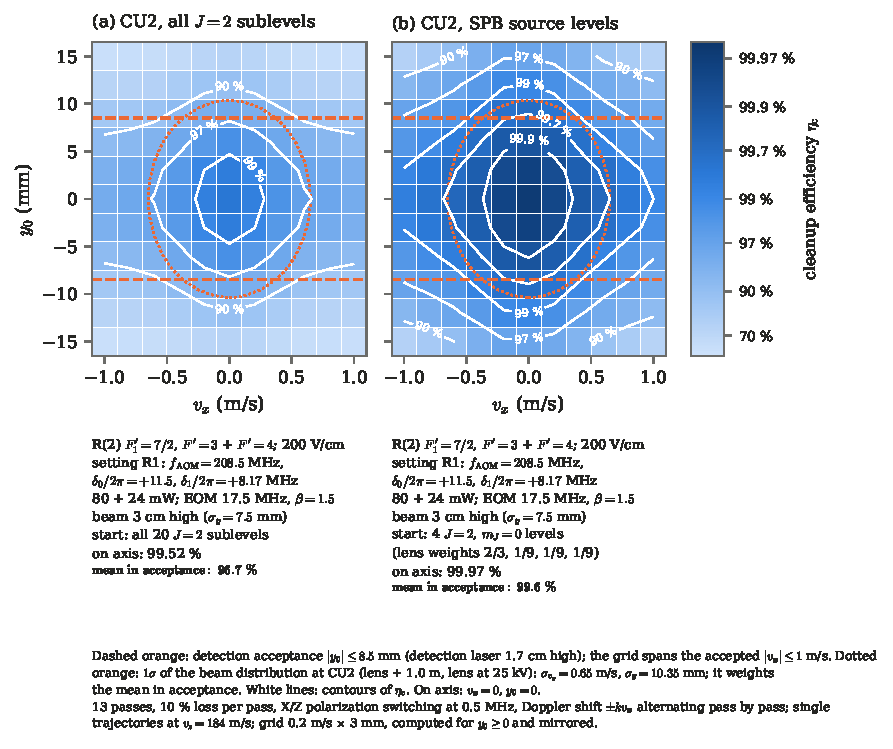
\includegraphics[width=0.9\textwidth]{cleanup_map_vx_y_CU2_current.pdf}
  \caption[CU2 at the present conditions: cleanup versus $v_x$ and $y_0$]{CU2 at the present
  conditions, setting R1 ($\fAOM=\SI{208.5}{MHz}$, $\delta_0/2\pi=+\SI{11.5}{MHz}$), \SI{3}{cm}
  beam, 80 + \SI{24}{mW}: cleanup versus transverse velocity and position from (a) all 20 $J=2$
  sublevels and (b) the four SPB source levels (coarse grid, mirrored in $y_0$). Dashed lines:
  detection acceptance; dotted ellipse: $1\sigma$ of the beam distribution at CU2. The conditions
  and the mean in acceptance are given under each map.}
  \label{fig:j2_doppler}
\end{figure}

% =====================================================================
\chapter{Numerical checks}
\label{ch:checks}

\begin{itemize}
  \item \textbf{Trace.} $\mathrm{Tr}\,\rho$ stays one to better than $10^{-14}$ in every
        model: no population leaves the modelled manifold.
  \item \textbf{Reproducibility.} The CU1 coarse and fine detuning scans, run separately,
        agree exactly at their four common points.
  \item \textbf{Tolerance.} At \SI{200}{V/cm} and $(+18.5,-\SI{6.5}{MHz})$, a point with much
        population left, the single trajectory with rtol $10^{-7}$ leaves 0.07125 in $J=2$ and
        the scan with rtol $10^{-6}$ leaves 0.07062, a difference of $6\times10^{-4}$. At the
        optimum of the two-dimensional scan the difference is only $3\times10^{-5}$
        (Table~\ref{tab:j2_confirm}), so the scan tolerance is adequate where it matters.
  \item \textbf{$\Lambda$-doublet partner.} Effect on the CU1 cleanup: $6\times10^{-6}$.
  \item \textbf{Package version.} A CU1 map computed with \code{centrex-tlf} 0.2.5 and 0.3.0 agrees to
        $1.2\times10^{-6}$; the \SI{2}{cm} test-condition runs use 0.3.0.
  \item \textbf{State identification.} No ambiguity warning at 150 and \SI{200}{V/cm}; one at
        \SI{250}{V/cm} (two states, margin 0.012).
  \item \textbf{Cross-coupling.} All neglected couplings between the two CU2 beams and the
        other excited level are detuned by more than \SI{50}{MHz} at every scanned point, the
        minimum being at $\delta_0/2\pi=\SI{5}{MHz}$, $\fAOM=\SI{185}{MHz}$, and by \SI{63}{MHz}
        at the optimum (Sec.~\ref{sec:couplings}).
\end{itemize}

Still to be done: convergence in $J_{\max}$ at \SI{200}{V/cm} for the eigenvectors (not only
the energies). Photon numbers from the running integral are available for the two CU2 optima
(Sec.~\ref{sec:j2_traj}); the other photon numbers in this report use the trapezoidal rule on
the \SI{1}{\micro\second} output grid.

% =====================================================================
\chapter{Conclusions and outlook}
\label{ch:conclusion}

\begin{table}[htbp]
  \centering
  \caption{Main results. Simulations use the baseline of Table~\ref{tab:baseline}; the CU1 test rows
  are measured with R(1) $F'=3$ detection unless stated.}
  \label{tab:summary}
  \small
  \begin{tabularx}{\textwidth}{Lr}
    \toprule
    quantity & value \\
    \midrule
    \multicolumn{2}{l}{\emph{CU1 simulation} ($\sigma_{v_x}=\SI{0.65}{m/s}$ assumed for the averages)} \\
    CU1: cleanup on axis at \SI{80}{mW}, $+\SI{20.2}{MHz}$, \SI{150}{V/cm} & \SI{99.96}{\percent} \\
    CU1: detuning window for $\etac>\SI{99.9}{\percent}$ (on axis) & \SI{0.6}{MHz} \\
    CU1: $|v_x|$ for $\etac>\SI{99.9}{\percent}$ / $>\SI{99}{\percent}$ (on axis, $+\SI{20.2}{MHz}$) & 0.2 / \SI{0.4}{m/s} \\
    CU1: set point, from the average over the transverse distribution & $+\SI{19.0}{MHz}$ \\
    CU1: mean in acceptance at $+\SI{19.0}{MHz}$, \SI{80}{mW}, \SI{3}{cm} / \SI{50}{mW}, \SI{2}{cm} & \SI{98.7}{\percent} / \SI{96.5}{\percent} \\
    CU1: same, \SI{50}{mW}, \SI{2}{cm}, AP1 triplet / singlet start & \SI{98.65}{\percent} / \SI{99.68}{\percent} \\
    CU1: tolerance on the laser tilt (antiparallel passes) & $\lesssim\SI{1}{mrad}$ \\
    \midrule
    \multicolumn{2}{l}{\emph{CU1 test on the SPB setup} (\SI{50}{mW}, \SI{2}{cm}, \SI{156}{V/cm}, AP1 on)} \\
    CU1: best cleanup (alignment C, RC on $F'=2$) & \SI{97.4(2)}{\percent} \\
    CU1: power exponent $a$ in $r=\exp(-kP^a)$ & $0.45\pm0.03$ \\
    CU1: $\sigma_{v_x}$ of the detected $J=1$ molecules (Doppler scan) & \SI{1.28(3)}{m/s} \\
    CU1: remaining at \SI{50}{mW}, model (17 passes, \SI{3.5}{\percent}/pass, \SI{1.28}{m/s}) / data & 0.031 / 0.032 \\
    CU1: predicted remaining for the final experiment ($|v_x|\leq\SI{0.22}{m/s}$) & $2\times10^{-5}$--$3\times10^{-4}$ \\
    CU1: measured optimum below the predicted set point (UV) & 4--\SI{6}{MHz} \\
    CU1: with Q(1) $F_1'=1/2$, $F'=1$ detection (RC on $F'=1$) & \SI{95.1(4)}{\percent} \\
    \midrule
    \multicolumn{2}{l}{\emph{CU2 simulation} (\code{centrex-tlf} 0.2.5)} \\
    CU2: $F'=4$ minus $F'=3$ main resonance at 200 / \SI{250}{V/cm} & 211.83 / \SI{219.93}{MHz} \\
    CU2, \SI{200}{V/cm}: reachable $(\delta_1-\delta_0)/2\pi$ for $\fAOM=200\pm\SI{15}{MHz}$ & $-26.83$ to $+\SI{3.17}{MHz}$ \\
    CU2, \SI{200}{V/cm}: cleanup at the former detunings $(+18.5,-\SI{6.5}{MHz})$ & \SI{92.9}{\percent} \\
    CU2, \SI{200}{V/cm}: best at $\fAOM=\SI{186.83}{MHz}$ (laser-frequency scan) & \SI{99.33}{\percent} \\
    CU2, \SI{200}{V/cm}: optimum $\delta_0/2\pi=+\SI{11.5}{MHz}$, $\fAOM=\SI{191.0}{MHz}$ (rtol $10^{-7}$) & \SI{99.85}{\percent} \\
    CU2, \SI{200}{V/cm}: second optimum $\delta_0/2\pi=+\SI{11.5}{MHz}$, $\fAOM=\SI{208.5}{MHz}$ & \SI{99.80}{\percent} \\
    CU2, \SI{200}{V/cm}: width of the optimum at \SI{99}{\percent} (laser / AOM frequency) & 2 / \SI{2.5}{MHz} \\
    CU2 reference at \SI{250}{V/cm} (Appendix~\ref{app:legacy}) & \SI{99.991}{\percent} \\
    CU2, R1 ($\fAOM=\SI{208.5}{MHz}$), \SI{3}{cm}, all 20 sublevels: mean in acceptance / on axis & \SI{96.7}{\percent} / \SI{99.5}{\percent} \\
    CU2, R1, SPB source levels: mean in acceptance / on axis & \SI{99.6}{\percent} / \SI{99.97}{\percent} \\
    CU2, R2 ($\fAOM=\SI{191.0}{MHz}$), all 20 sublevels / SPB source levels & \SI{96.1}{\percent} / \SI{99.35}{\percent} \\
    \bottomrule
  \end{tabularx}
\end{table}

On the beam axis CU1 removes \SI{99.96}{\percent} of the $J=1$ population with a single
\SI{80}{mW} beam and no phase modulation, as the design study anticipated, but the optimum is narrow
(\SI{0.6}{MHz} at the \SI{99.9}{\percent} level). In the multipass the Doppler shift alternates in
sign from pass to pass, so it cannot be compensated by the laser frequency, and CU1 is very sensitive
to the transverse velocity. Averaged over a transverse distribution, $+\SI{19.0}{MHz}$ is the best
detuning: there the laser is resonant with the eight SPB-related sublevels, which lie
\SI{2.4}{MHz} below the other four, for molecules with $|v_x|\approx\SI{0.5}{m/s}$, and these are
cleaned better than molecules at rest. With the lensed-beam distribution assumed before the test, the
model predicted \SI{98.7}{\percent} for \SI{80}{mW} in a \SI{3}{cm} beam and \SI{96.5}{\percent} for
\SI{50}{mW} in a \SI{2}{cm} beam within the detection acceptance, and more for the four levels
populated by AP1. A tilt of the laser acts like a shift of the transverse velocity and must stay
below about \SI{1}{mrad}.

The test on the SPB setup reached \SI{97.4(2)}{\percent} for the detected $F=2$ molecules at
\SI{50}{mW}, after the multipass had been realigned to about 17 passes and RC moved to P(2) $F'=2$.
Two measurements explain the residual. The power dependence is slow, $r=\exp(-kP^{0.45})$, the
signature of an inhomogeneous ensemble; and the detected $J=1$ molecules have
$\sigma_{v_x}=\SI{1.28}{m/s}$, twice the assumed value, because the lens hardly acts on them and the
test detection accepts $|v_x|>\SI{1}{m/s}$. With the measured distribution, the model with 17 passes
and \SI{3.5}{\percent} loss per pass reproduces the power dependence to within \SI{5}{\percent} at
30--\SI{50}{mW}, and the residual comes from $|v_x|>\SI{1}{m/s}$. For the acceptance of the final
experiment, $|v_x|\leq\SI{0.22}{m/s}$, the model predicts that CU1 removes more than
\SI{99.9}{\percent} of the $J=1$ population. Q(1) detection gives \SI{95.1(4)}{\percent}; because Q(1)
forms dark states during detection, its ratio is not the $J=1$ remaining fraction, and this
difference was not pursued. Open are the 4--\SI{6}{MHz} offset of the measured optimum from the
predicted set point and a direct test of the velocity interpretation.

For CU2 the change of field from 250 to \SI{200}{V/cm} invalidates the former set point,
because the relative position of the $F'=3$ and $F'=4$ manifolds moves by \SI{8}{MHz}. Since
the two beams are coupled by the AOM, the new optimum had to be found in laser frequency and AOM
frequency together, within $\fAOM=200\pm\SI{15}{MHz}$. The two-dimensional optimisation finds
\SI{99.85}{\percent} at $\delta_0/2\pi=+\SI{11.5}{MHz}$, $\fAOM=\SI{191.0}{MHz}$, confirmed with
tighter tolerances, and a nearly equivalent optimum (\SI{99.80}{\percent}) at
$\fAOM=\SI{208.5}{MHz}$, exactly one EOM period higher in $\fAOM$. Both work because the
comb of the $F'=4$ beam then lies at the same frequencies, with the roles of carrier and
first-order sideband exchanged, and these carry almost the same power at $\beta=1.5$
(Sec.~\ref{sec:j2_two_aom}). The remaining $J=2$
population is \SI{0.15}{\percent}, against \SI{0.67}{\percent} for the best point of the first
laser-frequency scan. Both optima are 2--\SI{3}{MHz} wide at the \SI{99}{\percent} level.

With the present \SI{3}{cm} beam and the transverse distribution (Sec.~\ref{sec:j2_doppler}),
the second optimum, $\fAOM=\SI{208.5}{MHz}$, is the more robust one and is recommended: it removes
\SI{96.7}{\percent} of a uniformly populated $J=2$ level and \SI{99.6}{\percent} of the population
in the SPB source levels within the detection acceptance. For CU2 the transverse position matters
more than the transverse velocity: the comb of the two phase-modulated beams tolerates Doppler
shifts of a few MHz, but the intensity at the edge of the acceptance is only about
\SI{50}{\percent} of the axial value.

Next steps:
\begin{enumerate}[itemsep=0pt,topsep=2pt]
  \item CU1: test the velocity interpretation with a narrower detection acceptance (slit or smaller
        probe), and recompute the best detuning, the EOM option and the tilt tolerance with the measured
        inputs ($\sigma_{v_x}=\SI{1.28}{m/s}$, 145--\SI{155}{m/s}, 17 passes).
  \item CU1: find the origin of the 4--\SI{6}{MHz} offset of the measured optimum, and characterise the
        loss per pass of the realigned multipass (\SI{3.5}{\percent} against \SI{4.5}{\percent} from two
        fits; Sec.~\ref{sec:exp_open}).
  \item Re-run the CU2 results with \code{centrex-tlf} 0.2.8 or later, in which the $J=2$ line positions
        move by up to about \SI{1}{MHz}.
  \item Use the beam simulation to give the transverse distribution of the molecules that reach
        the detection laser, at the CU1 and CU2 planes. This removes the approximation of
        applying the detection cut at the cleanup planes; the stored grids only need to be
        re-weighted.
  \item CU2: re-optimise $(\delta_0,\fAOM)$ for the \SI{3}{cm} beam with the transverse average,
        starting from R1, and scan the power split between the two beams. The stretched
        sublevels $|F_1=\tfrac52,F=3,m_F=\pm3\rangle$, pumped almost only by the \SI{24}{mW}
        $F'=4$ beam, limit the cleanup at low intensity (Sec.~\ref{sec:j2_traj}).
  \item Sensitivity of the CU2 optimum to the electric field (e.g.\ 198 and \SI{202}{V/cm}), which
        requires rebuilding the model, and the field uniformity across the cleanup region at
        \SI{200}{V/cm}.
  \item Correct the stored metadata of the CU1 run \code{detuning\_withoutP-\_-20to\_100MHz},
        which records \code{retain\_opposite\_parity\_levels=True} although it was run with
        the 21-level model.
\end{enumerate}

% =====================================================================
\appendix

\chapter{Model parameters}
\label{app:params}

\begin{table}[!ht]
  \centering
  \caption{Parameters of the simulation.}
  \label{tab:params}
  \footnotesize
  \begin{tabularx}{\textwidth}{lLl}
    \toprule
    symbol & quantity & value \\
    \midrule
    \multicolumn{3}{l}{\emph{fields and molecule}} \\
    $E$ & electric field along $z$ & \SI{150}{V/cm} (CU1), \SI{200}{V/cm} (CU2) \\
    $B$ & magnetic field along $z$ & \SI{1e-3}{\gauss} \\
    $\Gamma$ & $B$-state decay rate & \SI{1.0101e7}{s^{-1}} ($\Gamma/2\pi=\SI{1.608}{MHz}$) \\
    $\Dxb$ & $X$--$B$ transition dipole moment & \SI{2.6675506e-30}{C\,m} \\
    $J_{\max}$ & rotational truncation of $X$ and $B$ & 4 (CU1), 5 (CU2) \\
    \midrule
    \multicolumn{3}{l}{\emph{trajectory}} \\
    $v$ & forward velocity & \SI{184}{m/s} (CU1 test comparison: \SI{145}{m/s}) \\
    $v_x$ & transverse velocity & $-1\ldots+\SI{1}{m/s}$ scanned \\
    $k_Lv_x/2\pi$ & Doppler shift, sign alternating per pass & \SI{3.68}{MHz} per m/s \\
    $y_0$ & transverse offset & $0\ldots\SI{15}{mm}$ scanned (mirrored) \\
    $\sigma_{v_x}$ & transverse velocity spread (beam sim., \SI{25}{kV}) & \SI{0.65}{m/s}, both stages \\
    & detected $J=1$ in the CU1 test (Doppler scan) & \SI{1.28}{m/s} \\
    $\sigma_y$ & beam size (beam sim., \SI{25}{kV}) & \SI{10.95}{mm} (CU1), \SI{10.35}{mm} (CU2) \\
    & detection acceptance & $|v_x|\leq\SI{1}{m/s}$, $|y_0|\leq\SI{8.5}{mm}$ \\
    & first assumption (Sec.~\ref{sec:j1_avg}) & $v_x$: \SI{1.8}{m/s} FWHM; $y_0$ uniform in \SI{15}{mm} \\
    $L_{\mathrm{IR}}$, $T$ & length and duration of the interaction region & \SI{5}{cm}, \SI{271.7}{\micro\second} \\
    \midrule
    \multicolumn{3}{l}{\emph{laser beam}} \\
    & number of passes & 13 (CU1 test model: 17; two-pass test: 2) \\
    $s_n$ & pass centres & $n\times\SI{3.5}{mm}$, $n=1\ldots13$ \\
    $L$ & loss per pass & \SI{10}{\percent} (CU1 test fits: 3.5--\SI{4.5}{\percent}) \\
    $\sigs$ & Gaussian width along the beam & \SI{0.75}{mm} (\SI{3}{mm} full $4\sigma$) \\
    $\sigy$ & Gaussian width transverse & \SI{12}{mm} (CU1, \SI{4.8}{cm}), \SI{6}{mm} (CU2, \SI{2.4}{cm}) \\
    & present beam height, both stages & \SI{3}{cm} ($\sigy=\SI{7.5}{mm}$), constant power; CU1 test: \SI{2}{cm} \\
    $\wpol/2\pi$ & polarization switching frequency & \SI{0.5}{MHz}, square wave, X/Z \\
    \midrule
    \multicolumn{3}{l}{\emph{CU1}} \\
    & transition & R(1) $F_1'=5/2$, $F'=2$ \\
    $P$ & laser power & \SI{80}{mW} (scans 10--\SI{110}{mW}); test: \SI{50}{mW} \\
    $E$ & field in the CU1 test & \SI{156}{V/cm} (model: \SI{150}{V/cm}) \\
    $\delta/2\pi$ & detuning: set point / on-axis optimum & $+\SI{19.0}{MHz}$ / $+\SI{20.2}{MHz}$ \\
    & optional phase EOM (not adopted) & \SI{1.6}{MHz}; best $\beta=1.5$ at $+\SI{20.0}{MHz}$ \\
    $m$ & main-pair matrix element & 0.1004 \\
    \midrule
    \multicolumn{3}{l}{\emph{CU2}} \\
    & transitions & R(2) $F_1'=7/2$, $F'=3$ and $F'=4$ \\
    $P_0$, $P_1$ & beam powers & \SI{80}{mW}, \SI{24}{mW} \\
    $\wmod/2\pi$, $\beta$ & phase modulation, common to both beams & \SI{17.5}{MHz}, 1.5 \\
    $\fAOM$ & AOM frequency (beam separation) & $200\pm\SI{15}{MHz}$ \\
    $\Dmain$ & separation of the main resonances & \SI{211.83}{MHz} (\SI{200}{V/cm}) \\
    $\delta_0/2\pi$, $\fAOM$ & optimum (laser, AOM) & $+\SI{11.5}{MHz}$, \SI{191.0}{MHz} ($\delta_1/2\pi=-\SI{9.33}{MHz}$) \\
    $m_0$, $m_1$ & main-pair matrix elements & 0.0948, 0.2286 \\
    \midrule
    \multicolumn{3}{l}{\emph{integration}} \\
    & method & \code{dopri5}, Rust, \code{expanded\_sparse}, \code{decomposed} \\
    & initial step, tolerances & \SI{2}{ns}; rtol $10^{-7}$, atol $10^{-9}$ (CU2 scans: $10^{-6}$, $10^{-8}$) \\
    \bottomrule
  \end{tabularx}
\end{table}

\chapter{Line positions of the CU1 test}
\label{app:exp_lines}

Table~\ref{tab:exp_lines} lists the laser frequencies found on the SPB setup. Frequencies are those
of the IR lasers read on the wavemeter; the UV frequency is four times the IR frequency, and the
IR frequency changes by about $-\SI{1}{MHz}$ per MHz of NLTL frequency. Figures~\ref{fig:exp_rc},
\ref{fig:exp_r1line} and~\ref{fig:exp_q1line} show the scans.

\begin{table}[htbp]
  \centering
  \caption[Line positions of the CU1 test]{Line positions found in the CU1 test. Offsets are from the
  transition-finder values, in the IR.}
  \label{tab:exp_lines}
  \small
  \begin{tabularx}{\textwidth}{lccL}
    \toprule
    line & IR frequency & NLTL & remarks \\
    \midrule
    RC P(2) $F_1'=3/2$, $F'=2$ & \SI{275842.0401}{GHz} & \SI{1810.0}{MHz} & Lorentzian FWHM
      \SI{6.2}{MHz}; $+\SI{1.4(1)}{MHz}$ \\
    RC P(2) $F_1'=3/2$, $F'=1$ & -- & about \SI{1886}{MHz} & former setting; possibly off centre
      (Fig.~\ref{fig:exp_rc}) \\
    CU1 R(1) $F_1'=5/2$, $F'=2$ & \SI{275855.3799}{GHz} & \SI{2466.0}{MHz} & final run, \SI{156}{V/cm};
      main pair $+\SI{9.1}{MHz}$ \\
    Det2 R(1) $F_1'=5/2$, $F'=3$ & \SI{275855.4647}{GHz} & \SI{2178.8}{MHz} & $+26$ to $+\SI{29}{MHz}$;
      FWHM \SI{4.5}{MHz} at \SI{30}{mW} \\
    Det2 Q(1) $F_1'=1/2$, $F'=1$ & \SI{275845.27034}{GHz} & \SI{2385.78}{MHz} & $+\SI{21.8}{MHz}$;
      Gaussian width $\sigma_G=\SI{1.24}{MHz}$ \\
    Det2 Q(1) $F_1'=3/2$, $F'=1$ & -- & about \SI{1990}{MHz} & not usable: the $+1$ and 0 orders of the
      serrodyne coincide there \\
    \bottomrule
  \end{tabularx}
\end{table}

\begin{figure}[htbp]
  \centering
  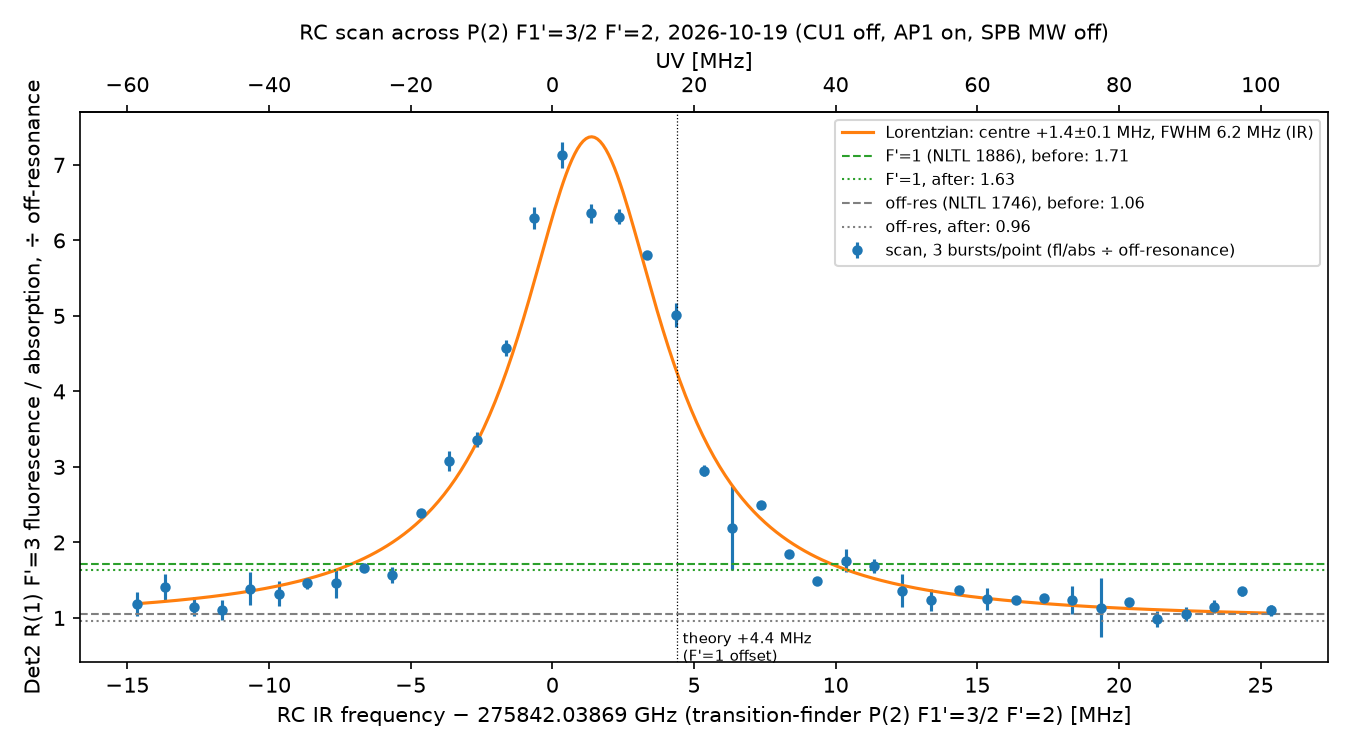
\includegraphics[width=0.72\textwidth]{experiment/exp_B1_rc_p2f2_scan.png}
  \caption[CU1 test: RC line]{RC scan across P(2) $F_1'=3/2$, $F'=2$ (10-19; CU1 off, AP1 on, SPB
  microwaves off): Det2 R(1) $F'=3$ signal relative to its off-resonance value versus the RC IR
  frequency, with a Lorentzian fit. Horizontal lines: the signal at the former $F'=1$ setting (NLTL
  \SI{1886}{MHz}) and off resonance, before and after the scan.}
  \label{fig:exp_rc}
\end{figure}

\begin{figure}[htbp]
  \centering
  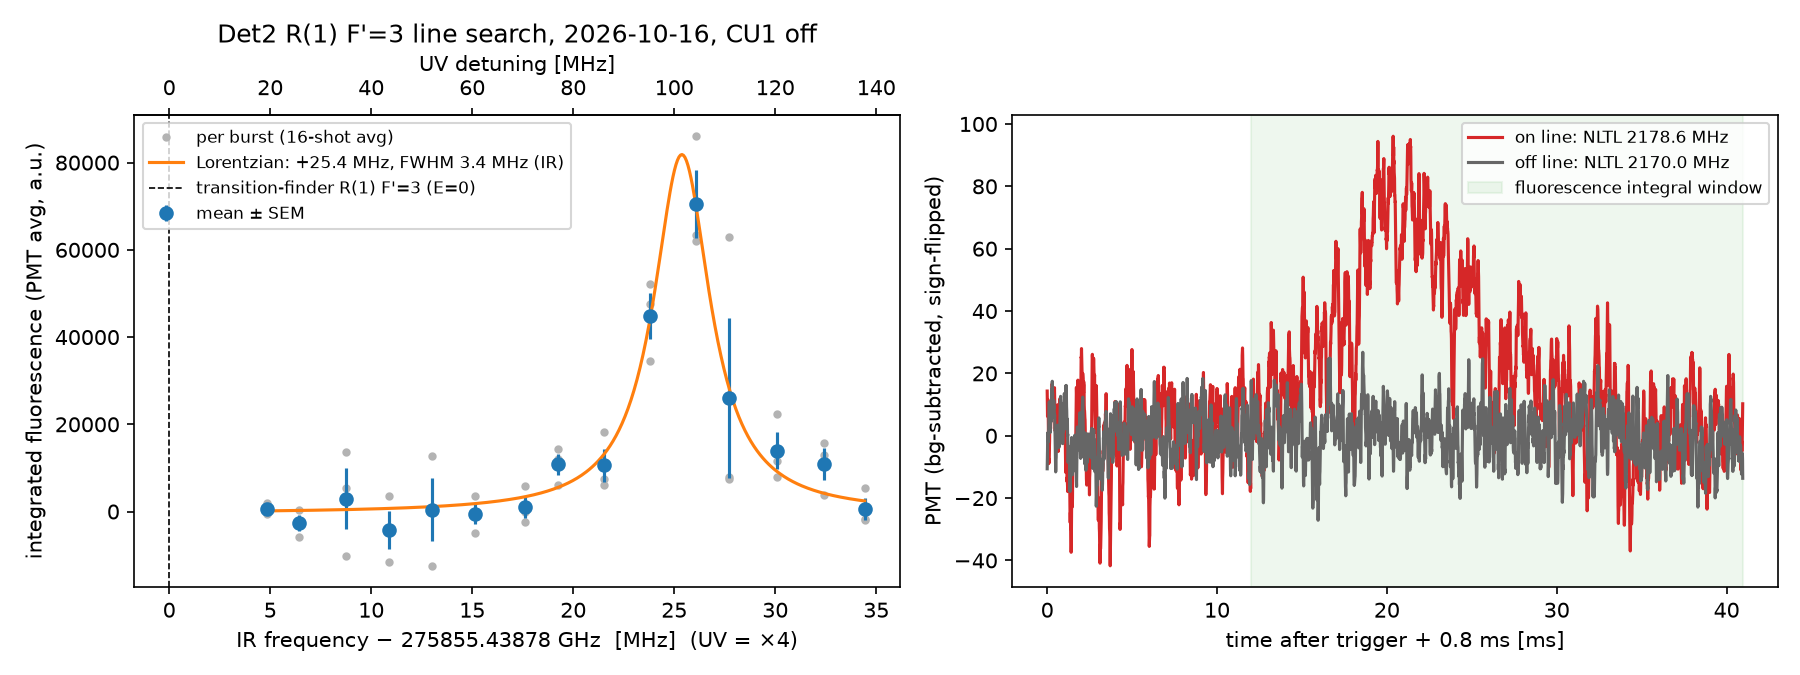
\includegraphics[width=\textwidth]{experiment/exp_B3_det2_r1f3_line_search.png}
  \caption[CU1 test: Det2 R(1) $F'=3$ line search]{Det2 R(1) $F'=3$ line search (10-16, CU1 off). Left:
  integrated fluorescence versus IR frequency, with a Lorentzian fit and the transition-finder value at
  zero field. Right: PMT traces on and off the line, with the integration window.}
  \label{fig:exp_r1line}
\end{figure}

\begin{figure}[htbp]
  \centering
  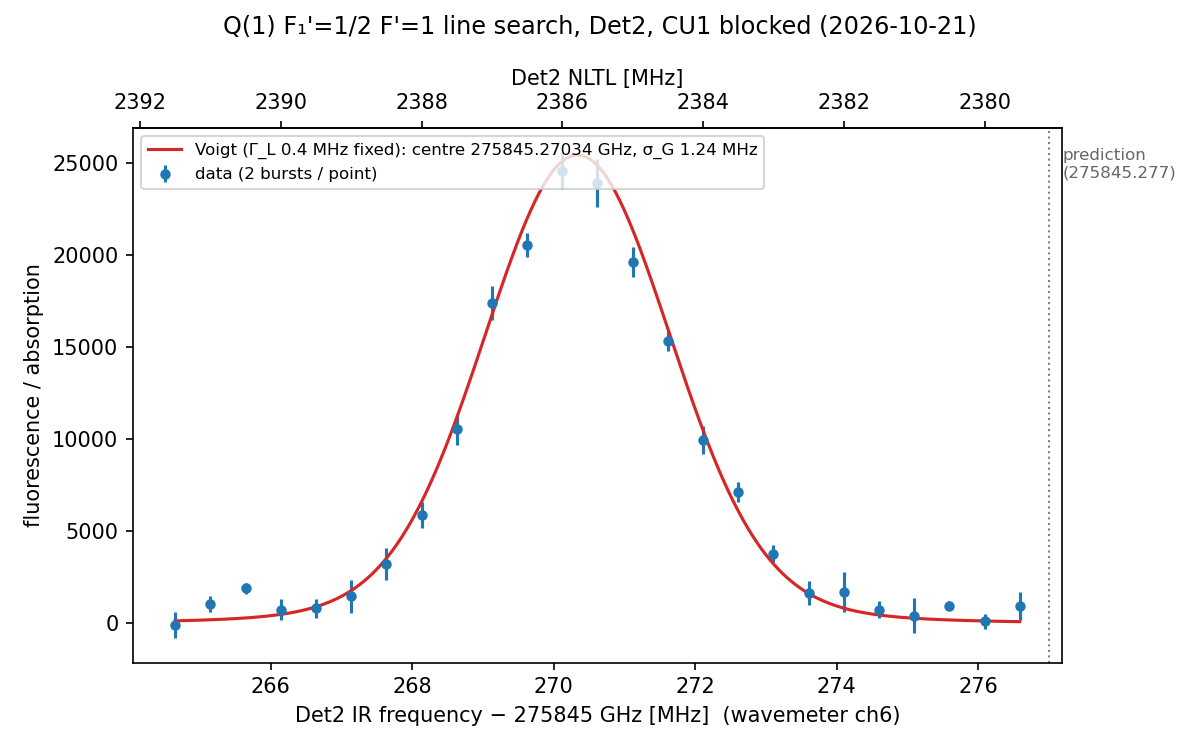
\includegraphics[width=0.7\textwidth]{experiment/exp_B7_det2_q1f1_line_search.png}
  \caption[CU1 test: Det2 Q(1) $F_1'=1/2$, $F'=1$ line search]{Det2 Q(1) $F_1'=1/2$, $F'=1$ line search
  (10-21, CU1 blocked): fluorescence over absorption versus IR frequency (top axis: NLTL), with a Voigt
  fit ($\Gamma_L=\SI{0.4}{MHz}$ fixed). Dotted line: the transition-finder value corrected by the offset
  measured on R(1) $F'=3$.}
  \label{fig:exp_q1line}
\end{figure}

\chapter{Reference results at \SI{250}{V/cm}}
\label{app:legacy}

These CU2 results were obtained before the operating field was changed to \SI{200}{V/cm}.
They use the same 56-level two-transition model and the same baseline beam parameters, and are
kept as a reference only.

\begin{itemize}
  \item Laser-frequency scan at fixed $\fAOM=\SI{194.93}{MHz}$
        ($(\delta_1-\delta_0)/2\pi=-\SI{25}{MHz}$), combined from three runs covering
        $\delta_0/2\pi=-58.5$ to $+\SI{141.5}{MHz}$ in \SI{1}{MHz} steps (one gap, 100.5 to
        \SI{102.5}{MHz}): best $\etac=\SI{99.991}{\percent}$ at $(+18.5,-\SI{6.5}{MHz})$
        (Fig.~\ref{fig:legacy}). Along this direction the cleanup falls to
        \SI{99.94}{\percent} at $-\SI{1}{MHz}$ and \SI{99.83}{\percent} at $+\SI{1}{MHz}$ from the
        optimum, and to \SI{99.03}{\percent} and \SI{98.68}{\percent} at $\mp\SI{2}{MHz}$.
  \item $3\times3$ grid around this point (Table~\ref{tab:legacy_grid}).
\end{itemize}

\begin{table}[htbp]
  \centering
  \caption[CU2 at \SI{250}{V/cm}: $3\times3$ detuning grid]{CU2 at \SI{250}{V/cm}: cleanup
  efficiency (\%) on a $3\times3$ grid (run \code{Fprime3\_Fprime4\_detuning}).}
  \label{tab:legacy_grid}
  \small
  \begin{tabular}{lccc}
    \toprule
    & $\delta_1/2\pi=-\SI{7.5}{MHz}$ & $-\SI{6.5}{MHz}$ & $-\SI{5.5}{MHz}$ \\
    \midrule
    $\delta_0/2\pi=+\SI{17.5}{MHz}$ & 99.944 & 99.870 & 99.519 \\
    $\delta_0/2\pi=+\SI{18.5}{MHz}$ & 99.984 & \textbf{99.991} & 99.958 \\
    $\delta_0/2\pi=+\SI{19.5}{MHz}$ & 99.801 & 99.918 & 99.833 \\
    \bottomrule
  \end{tabular}
\end{table}

\begin{figure}[htbp]
  \centering
  \figplaceholder{CU2_250V_laser_frequency_scan_combined.pdf}
  \caption[CU2 at \SI{250}{V/cm}: combined laser-frequency scan]{CU2 at \SI{250}{V/cm}:
  cleanup versus $\delta_0$ at fixed $\fAOM=\SI{194.93}{MHz}$ (run
  \code{correlated\_detuning\_shared\_offset\_boarder\_combined}). Reference only.}
  \label{fig:legacy}
\end{figure}

\paragraph{Single-transition variant.} A variant with only R(2) $F'=3$, in which one laser is
split by an AOM into two phase-modulated tones (\SI{80}{\percent} and \SI{20}{\percent} of
\SI{100}{mW}) offset by $\Delta_{\mathrm{AOM}}$, was simulated at \SI{250}{V/cm} with a
38-level model. At $\delta/2\pi=\Delta_{\mathrm{AOM}}/2\pi=\SI{18.5}{MHz}$ it reaches
$\etac=\SI{99.05}{\percent}$ with $\Ngam=1.53$, with the removed molecules in $J=3$
(\SI{59.9}{\percent}), $J=4$ (\SI{37.2}{\percent}) and $J=5$ (\SI{1.9}{\percent}). It
corresponds to step~2 of the design (Sec.~\ref{sec:design_cu2}), which the design study found
limited by dark states, and is not pursued further.

\chapter{Code and data}
\label{app:code}

\begin{table}[htbp]
  \centering
  \caption{Notebooks and scripts.}
  \label{tab:code}
  \small
  \begin{tabularx}{\textwidth}{lL}
    \toprule
    file & contents \\
    \midrule
    \code{SPB\_cleanup\_J1-J2F2.ipynb} & CU1: build, single trajectory, detuning,
      power and geometry scans, HDF5 readback, optimum and re-run \\
    \code{SPB\_cleanup\_J2\_J3F4\_opposite\_parity.ipynb} & CU2 two-transition scheme:
      build, single trajectory, detuning scans, combination of runs \\
    \code{SPB\_cleanup\_J2\_J3F3\_2laser.ipynb} & CU2 single-transition variant
      (\SI{250}{V/cm}; not pursued) \\
    \code{scripts/scan\_progress.py} & chunked grid scan with progress bar
      (\code{grid\_scan\_with\_progress}) \\
    \code{scripts/scan\_hdf.py} & HDF5 storage with metadata (\code{save\_scan\_hdf},
      \code{load\_scan\_hdf}) \\
    \code{scripts/migrate\_j2\_j3f4\_notebook.py} & one-off migration of the CU2 notebook
      from the Julia workflow \\
    \code{scripts/refactor\_scan\_cells.py} & one-off rewrite of the scan sections \\
    \code{scripts/cu2\_laser\_aom\_scan.py} & CU2 two-dimensional scan in laser and AOM frequency
      at \SI{200}{V/cm}: stages \code{test}, \code{coarse}, \code{fine}, \code{confirm};
      checkpoints in \code{tmp/cu2\_laser\_aom\_scan/} \\
    \code{scripts/plot\_cu2\_laser\_aom\_map.py} & figures of the CU2 2D scan
      (Figs.~\ref{fig:j2_map} and~\ref{fig:j2_fine}) \\
    \code{scripts/cu2\_optimum\_trajectories.py} & trajectories and photon numbers at the two CU2
      optima, and their figures (Figs.~\ref{fig:j2_opt_pop} and~\ref{fig:j2_opt_sub}) \\
    \code{scripts/cu2\_level\_scheme.py} & CU2 excited-sublevel positions and coupling strengths
      at \SI{200}{V/cm}, with the laser combs of the two optima (Fig.~\ref{fig:j2_scheme}) \\
    \code{scripts/cleanup\_spb\_doppler.py} & CU1 model with Doppler shift and optional EOM
      (\code{build\_cu1}); SPB-related levels; $(v_x,y_0)$ maps for CU1 and CU2 \\
    \code{scripts/plot\_cu1\_doppler\_map.py} & Fig.~\ref{fig:j1_doppler} \\
    \code{scripts/cu1\_eom\_doppler\_scan.py} & CU1 with the \SI{1.6}{MHz} EOM: $\beta\times\delta\times v_x$
      scan, $y_0$ averages, full map; checkpoints in \code{tmp/cu1\_eom\_doppler/} \\
    \code{scripts/plot\_cu1\_eom.py} & figure of the EOM study (Sec.~\ref{sec:j1_eom}; not reproduced here) \\
    \code{scripts/cu1\_trajectories.py} & CU1 trajectories per starting sublevel at $+19.0$ and
      $+\SI{20.2}{MHz}$ (Fig.~\ref{fig:j1_traj19}) \\
    \code{scripts/cleanup\_level\_diagrams.py} & field-dressed level diagrams with laser lines and
      per-level residuals (slides only) \\
    \code{scripts/cu1\_3cm\_scan.py} & CU1 with the \SI{3}{cm} beam: detuning scan averaged over the
      acceptance, full map at the set point (Secs.~\ref{sec:j1_avg} and~\ref{sec:j1_present}) \\
    \code{scripts/cu2\_doppler\_scan.py} & CU2 $(v_x,y_0)$ maps at R1 and R2, \SI{3}{cm} beam,
      two initial states (Table~\ref{tab:j2_doppler}) \\
    \code{scripts/plot\_cleanup\_maps\_current.py} & Figs.~\ref{fig:j1_present} and~\ref{fig:j2_doppler};
      mean in acceptance with the beam-simulation weights \\
    \bottomrule
  \end{tabularx}
\end{table}

\begin{table}[htbp]
  \centering
  \caption[Scripts for the CU1 test conditions]{Scripts for the CU1 test conditions, the comparison with the test and the detection lines.}
  \label{tab:code_test}
  \small
  \begin{tabularx}{\textwidth}{lL}
    \toprule
    file & contents \\
    \midrule
    \code{scripts/cu1\_conditions\_scan.py} & CU1 at a chosen power and beam height: detuning scan and full
      map (Table~\ref{tab:j1_conditions}, Fig.~\ref{fig:j1_present}) \\
    \code{scripts/cu1\_tilt\_scan.py} & CU1 with a tilted laser: extended $v_x$ range, analysis and
      Fig.~\ref{fig:j1_tilt} \\
    \code{scripts/cu1\_ap1\_start.py} & CU1 from the AP1 levels and the R(1) reading
      (Sec.~\ref{sec:j1_ap1}) \\
    \code{scripts/cu1\_two\_pass\_test.py} & two-pass test of the laser tilt (Fig.~\ref{fig:j1_twopass}) \\
    \code{scripts/detection\_level\_diagrams.py} & probe model and level diagrams of the two detection
      lines (slides only) \\
    analysis of the CU1 test & scripts and raw data outside this repository; the analysis figures used
      in Chapter~\ref{ch:j1_exp} and Appendix~\ref{app:exp_lines} are in \code{figures/experiment/} \\
    \bottomrule
  \end{tabularx}
\end{table}

\begin{table}[htbp]
  \centering
  \caption[Stored scan runs, CU1]{Stored scan runs used in this report, CU1 (best cleanup in the run). Both
  files are in \code{results/}; \code{results/scan\_results.md} lists every run with its axes and
  conditions and is regenerated by \code{scripts/write\_results\_index.py}.}
  \label{tab:runs}
  \small
  \begin{tabularx}{\textwidth}{lLr}
    \toprule
    run & content & best $\etac$ \\
    \midrule
    \multicolumn{3}{l}{\code{results/SPB\_J1\_cleanup\_scans.h5} (CU1, \SI{150}{V/cm})} \\
    \code{detuning\_withoutP-\_-20to\_100MHz} & 21 levels; $-20\ldots100$\,MHz, 1\,MHz & 99.9275\,\% \\
    \code{detuning\_board\_-20to\_100MHz} & 26 levels; $-20\ldots100$\,MHz, 1\,MHz & 99.9269\,\% \\
    \code{detuning\_fine} & 26 levels; $19\ldots22$\,MHz, 0.1\,MHz & 99.963\,\% \\
    \code{power\_detuning\_no\_phase\_eom} & 26 levels; 10--110\,mW $\times$ $-16\ldots30$\,MHz & 99.955\,\% \\
    \code{vertical\_position\_beam\_diameter} & earlier configuration; $y_0\times4\sigy$ at constant peak intensity & 99.877\,\% \\
    \code{doppler\_cu1\_spb} & 26 levels; $+20.2$\,MHz; $v_x$ $-1\ldots1$\,m/s $\times$ $y_0$ 0--15\,mm; SPB-related start & 99.970\,\% \\
    \code{doppler\_cu1\_uniform} & as above, uniform 12-level start & 99.968\,\% \\
    \code{doppler\_cu1\_spb\_eom1p6MHz\_beta1p5\_det20MHz} & as \code{doppler\_cu1\_spb}, \SI{1.6}{MHz} EOM, $\beta=1.5$, $+20.0$\,MHz & 99.49\,\% \\
    \code{eom\_beta\_detuning\_vx\_cu1\_spb\_4p8cm} & \SI{1.6}{MHz} EOM: $\beta\times\delta\times v_x$ at $y_0=0$ (NaN: not computed; Sec.~\ref{sec:j1_eom}) & -- \\
    \code{doppler\_cu1\_spb\_4p8cm\_coarse\_settings} & coarse $v_x\times y_0$ for the 9 settings of the averages (Sec.~\ref{sec:j1_avg}) & -- \\
    \code{trajectories\_cu1\_vx0\_19p0\_20p2MHz\_4p8cm} & populations vs time per starting sublevel (Fig.~\ref{fig:j1_traj19}) & -- \\
    \code{per\_level\_cu1\_20p2MHz\_4p8cm} & remaining per starting sublevel, on axis & -- \\
    \code{per\_state\_cu1\_spb\_20p2MHz\_4p8cm} & the 8 SPB-related levels, with destinations & -- \\
    \bottomrule
  \end{tabularx}
\end{table}

\begin{table}[htbp]
  \centering
  \caption[Stored scan runs, CU1 present and test conditions]{Stored scan runs used in this report, CU1 at the present (\SI{3}{cm}, \SI{80}{mW}) and test (\SI{2}{cm}, \SI{50}{mW}) conditions (\code{results/SPB\_J1\_cleanup\_scans.h5}; best cleanup in the run).}
  \label{tab:runs_present}
  \small
  \begin{tabularx}{\textwidth}{lLr}
    \toprule
    run & content & best $\etac$ \\
    \midrule
    \code{doppler\_cu1\_spb\_3cm\_det19MHz} & \SI{3}{cm} beam, $+19.0$\,MHz, no EOM; $v_x\times y_0$, 0.1\,m/s $\times$ 1.5\,mm & 99.99\,\% \\
    \code{detuning\_vx\_y\_cu1\_spb\_3cm\_coarse} & \SI{3}{cm} beam: $\delta\times v_x\times y_0$ (Sec.~\ref{sec:j1_avg}) & -- \\
    \code{detuning\_vx\_y\_cu1\_spb\_3cm\_coarse\_vx2} & as above, $v_x$ extended to $\pm\SI{2}{m/s}$ (laser tilt) & -- \\
    \code{detuning\_vx\_y\_cu1\_spb\_2cm\_50mW\_coarse} & \SI{50}{mW}, \SI{2}{cm} beam: $\delta\times v_x\times y_0$ (Table~\ref{tab:j1_conditions}) & -- \\
    \code{detuning\_vx\_y\_cu1\_spb\_2cm\_50mW\_coarse\_vx2} & as above, $v_x$ extended to $\pm\SI{2}{m/s}$ (Fig.~\ref{fig:j1_tilt}) & -- \\
    \code{doppler\_cu1\_spb\_2cm\_50mW\_det19MHz} & \SI{50}{mW}, \SI{2}{cm}, $+19.0$\,MHz; $v_x\times y_0$, 0.1\,m/s $\times$ 1.5\,mm & 99.990\,\% \\
    \code{doppler\_cu1\_ap1\_\{triplet,singlet\}\_2cm\_50mW\_det19MHz} & AP1 starts, final population of each $J=1$ sublevel on the $v_x\times y_0$ grid (Sec.~\ref{sec:j1_ap1}) & -- \\
    \bottomrule
  \end{tabularx}
\end{table}

\begin{table}[htbp]
  \centering
  \caption[Stored scan runs, CU2]{Stored scan runs used in this report, CU2 (best cleanup in the run; \code{results/SPB\_J2\_cleanup\_scans.h5}, 56 levels).}
  \label{tab:runs_j2}
  \small
  \begin{tabularx}{\textwidth}{lLr}
    \toprule
    run & content & best $\etac$ \\
    \midrule
    \code{correlated\_detuning\_shared\_offset\_200V} & \SI{200}{V/cm}; $\fAOM=186.83$\,MHz; offset $-10\ldots8$\,MHz, 2\,MHz & 99.33\,\% \\
    \code{laser\_AOM\_2D\_200V\_coarse\_2MHz} & \SI{200}{V/cm}; $\delta_0$ 5--23\,MHz $\times$ $\fAOM$ 185--215\,MHz, 2\,MHz & 99.79\,\% \\
    \code{laser\_AOM\_2D\_200V\_fine\_0p5MHz\_region1--3} & \SI{200}{V/cm}; $9\times9$ grids, 0.5\,MHz & 99.85\,\% \\
    \code{laser\_AOM\_2D\_200V\_confirm\_rtol1e-7} & \SI{200}{V/cm}; 3 best points, rtol $10^{-7}$ & 99.85\,\% \\
    \code{doppler\_cu2\_\{R1,R2\}\_\{uniform,spb\}\_3cm\_coarse} & \SI{200}{V/cm}, \SI{3}{cm} beam; $v_x\times y_0$, 0.2\,m/s $\times$ 3\,mm & 99.52--99.97\,\% \\
    \code{trajectories\_cu2\_R1\_R2\_2p4cm} & populations vs time at R1 and R2 (Figs.~\ref{fig:j2_opt_pop}, \ref{fig:j2_opt_sub}) & -- \\
    \code{per\_level\_cu2\_R1\_R2\_2p4cm} & remaining and leakage to $J=1$ per starting sublevel & -- \\
    \code{per\_state\_cu2\_spb\_R1\_R2\_2p4cm} & the 4 SPB source levels, with destinations & -- \\
    \code{level\_scheme\_cu2\_200V\_sublevels} & excited-sublevel table of Fig.~\ref{fig:j2_scheme} & -- \\
    \code{level\_scheme\_cu2\_200V\_pairs} & coupled-pair table of Fig.~\ref{fig:j2_scheme} & -- \\
    \code{Fprime3\_Fprime4\_detuning} & \SI{250}{V/cm}; $3\times3$ grid & 99.991\,\% \\
    \code{correlated\_detuning\_shared\_offset\_boarder\_combined} & \SI{250}{V/cm}; $\fAOM=194.93$\,MHz; combined & 99.991\,\% \\
    \bottomrule
  \end{tabularx}
\end{table}

A typical run consists of
\begin{enumerate}[itemsep=0pt,topsep=2pt]
  \item \code{lindblad.generate\_OBE\_system\_transitions} (build the OBE system);
  \item binding of the runtime parameters and \code{lindblad.prepare\_lindblad\_problem}
        (prepare once);
  \item \code{lindblad.solve\_lindblad} for single trajectories, or
        \code{grid\_scan\_with\_progress} and \code{lindblad.parameter\_scan} for scans;
  \item \code{save\_scan\_hdf} for storage.
\end{enumerate}
Stored runs are read back with \code{load\_scan\_hdf} without rebuilding the model.

% =====================================================================
\begin{thebibliography}{99}

\bibitem{Grasdijk2021}
O.~Grasdijk \emph{et al.}, ``CeNTREX: a new search for time-reversal symmetry violation in
the $^{205}$Tl nucleus,'' Quantum Sci.\ Technol.\ \textbf{6}, 044007 (2021),
arXiv:2010.01451.

\bibitem{CleanupTheory2024}
Y.~Yang, ``State Cleanup Theory,'' CeNTREX internal presentation (June 2024, updated 2026).

\bibitem{centrextlf}
O.~Grasdijk \emph{et al.}, \code{centrex-tlf}: TlF states, Hamiltonians, couplings and
optical Bloch equations for CeNTREX, versions 0.2.5 and 0.3.0,
\url{https://github.com/ograsdijk/CeNTREX-TlF}.

\bibitem{CU1GroupMeeting2026}
Y.~Yang, ``CU1 state cleanup of $J=1$ on the SPB setup,'' CeNTREX group meeting (2026-10-20).

\bibitem{Grasdijk2025AP}
O.~Grasdijk \emph{et al.}, ``Adiabatic passage of $^{205}$TlF with microwaves in a cryogenic
beam,'' arXiv:2511.16626.

\bibitem{Lindblad1976}
G.~Lindblad, ``On the generators of quantum dynamical semigroups,''
Commun.\ Math.\ Phys.\ \textbf{48}, 119 (1976).

\bibitem{Dormand1980}
J.~R. Dormand and P.~J. Prince, ``A family of embedded Runge--Kutta formulae,''
J.\ Comput.\ Appl.\ Math.\ \textbf{6}, 19 (1980).

\end{thebibliography}

\end{document}
